\documentclass[english, a4paper, 12pt, twoside]{book}

\usepackage[subpreambles=false]{standalone}



%%%%%%%%%%%%%%%%%%%%%%%%%%%%%%%%%%%%%%%%%%%%%%%%%%%%%%%%%%%%%%%%%%%%%

%% Réglage des fontes et typo    
\usepackage[utf8]{inputenc}		% LaTeX, comprend les accents !
\usepackage[T1]{fontenc}
\usepackage[english, french]{babel}


\usepackage[dvipsnames]{xcolor}  % Coloured text etc.
\usepackage{graphicx}
\usepackage{mathrsfs}

\usepackage{listings}
\definecolor{gray}{rgb}{0.4,0.4,0.4}
\definecolor{darkblue}{rgb}{0.0,0.0,0.6}
\definecolor{cyan}{rgb}{0.0,0.6,0.6}
\lstset{
  basicstyle=\ttfamily,
  columns=fullflexible,
  showstringspaces=false,
  commentstyle=\color{gray}\upshape
}
\lstdefinelanguage{XML}
{
  morestring=[b]",
  morestring=[s]{>}{<},
  morecomment=[s]{<?}{?>},
  stringstyle=\color{black},
  identifierstyle=\color{darkblue},
  keywordstyle=\color{cyan},
  morekeywords={diameter, name}% list your attributes here
}
\lstset{language=XML}

%%%%%%%%%%%%%%%%%%%%%%%%%%%%%%%%%%%%%%%%%%%%%%%%%%%%%%%%%%%%%%%%%%%%%

%% Apparence globale             
\usepackage[top=3cm, bottom=2cm, left=3cm, right=3cm,
			headheight=15pt]{geometry} 
\usepackage{fancyhdr}			% Entête et pieds de page
	\pagestyle{fancy}			% Indique que le style de la page sera justement fancy
	\lfoot[\thepage]{} %gauche du pied de page
	\cfoot{} %milieu du pied de page
	\rfoot[]{\thepage} %droite du pied de page
	\fancyhead[RO, LE] {}	
\usepackage{enumerate}
\usepackage{enumitem}
\usepackage[section]{placeins}	% Place un FloatBarrier à chaque nouvelle section
\usepackage{epigraph}
\usepackage[font={small}]{caption}
\usepackage[english]{minitoc}		% Mini table des matières, en français
	\setcounter{minitocdepth}{2}	% Mini-toc détaillées (sections/sous-sections)
\usepackage{pdflscape}				% Permet d'utiliser des pages au format paysage


%%%%%%%%%%%%%%%%%%%%%%%%%%%%%%%%%%%%%%%%%%%%%%%%%%%%%%%%%%%%%%%%%%%%%
% Biblio                        
%\makeatletter
%\patchcmd{\BR@backref}{\newblock}{\newblock(page~}{}{}	% Pour les back-references, affiche 'page' au lieu de 'p.'
%\patchcmd{\BR@backref}{\par}{)\par}{}{}
%\makeatother
	

%%%%%%%%%%%%%%%%%%%%%%%%%%%%%%%%%%%%%%%%%%%%%%%%%%%%%%%%%%%%%%%%%%%%%
% Tableau
\usepackage{array}
\usepackage{hhline}
\usepackage{adjustbox}
\usepackage{multirow,makecell}
\usepackage{color}
\usepackage{arydshln}

% Images
\usepackage{subfigure}

% Algo
\usepackage{algorithm}
\usepackage{algorithmic}

%%%%%%%%%%%%%%%%%%%%%%%%%%%%%%%%%%%%%%%%%%%%%%%%%%%%%%%%%%%%%%%%%%%%%
%% Mise en forme du texte        
\usepackage{xspace}
%\usepackage[load-configurations = abbreviations]{siunitx}
%	\DeclareSIUnit{\MPa}{\mega\pascal}
%	\DeclareSIUnit{\micron}{\micro\meter}
%	\DeclareSIUnit{\tr}{tr}
%	\DeclareSIPostPower\totheM{m}
%	\sisetup{
%	locale = FR,
%	  inter-unit-separator=$\cdot$,
%	  range-phrase=~\`{a}~,     	% Utilise le tiret court pour dire "de... à"
%	  range-units=single,  			% Cache l'unité sur la première borne
%	  }
%\usepackage{chemist}
%\usepackage[version=3]{mhchem}
\usepackage{textcomp}
\usepackage{numprint}

\usepackage{hyphenat}


\usepackage{times}
\usepackage{amsmath,amssymb,mathtools}
\usepackage{tikz-uml}
\usepackage{environ}

% to be able to scale tikzpicture
\makeatletter
\newsavebox{\measure@tikzpicture}
\NewEnviron{scaletikzpicturetowidth}[1]{%
  \def\tikz@width{#1}%
  \def\tikzscale{1}\begin{lrbox}{\measure@tikzpicture}%
  \BODY
  \end{lrbox}%
  \pgfmathparse{#1/\wd\measure@tikzpicture}%
  \edef\tikzscale{\pgfmathresult}%
  \BODY
}
\makeatother

%%%%%%%%%%%%%%%%%%%%%%%%%%%%%%%%%%%%%%%%%%%%%%%%%%%%%%%%%%%%%%%%%%%%%
%% Pour changer localement les marges

\newenvironment{changemargin}[2]{%
\begin{list}{}{%
\setlength{\leftmargin}{#1}%
\setlength{\rightmargin}{#2}%
\setlength{\listparindent}{\parindent}%
\setlength{\itemindent}{\parindent}%
\setlength{\parsep}{\parskip}%
}%
\item[]}{\end{list}}

\definecolor{ieeeblue}{RGB}{0,98,155}

\usepackage{bm}


\usepackage[sorting=none,
  style=alphabetic,
  backref=true,
  backend=biber,
  maxnames=6,
  minnames=1]{biblatex}

% \usepackage[
% backend=biber,
% style=numeric,
% ]{biblatex}
% recommended when using biblatex with babel
\usepackage{csquotes}

%% Navigation dans le document
\usepackage[pdftex,
  pdfborder={0 0 0},
  colorlinks=true,
  linkcolor=blue,
  citecolor=red,
  pagebackref=false,
  ]{hyperref} %Créera automatiquement les liens internes au PDF

% TODO notes
\usepackage{xargs}                      % Use more than one optional parameter in a new commands
\usepackage[dvipsnames]{xcolor}  % Coloured text etc.
% 
\usepackage[colorinlistoftodos,prependcaption,textsize=tiny]{todonotes}
\newcommandx{\unsure}[2][1=]{\todo[linecolor=red,backgroundcolor=red!25,bordercolor=red,#1]{#2}}
\newcommandx{\change}[2][1=]{\todo[linecolor=blue,backgroundcolor=blue!25,bordercolor=blue,#1]{#2}}
\newcommandx{\info}[2][1=]{\todo[linecolor=OliveGreen,backgroundcolor=OliveGreen!25,bordercolor=OliveGreen,#1]{#2}}
\newcommandx{\improvement}[2][1=]{\todo[linecolor=Plum,backgroundcolor=Plum!25,bordercolor=Plum,#1]{#2}}
\newcommandx{\thiswillnotshow}[2][1=]{\todo[disable,#1]{#2}}


% include all bib files separately.
% to use wildecard upgrade biber to 2.13
\addbibresource{bibfiles/these.bib}
\addbibresource{bibfiles/centroidal-est.bib}
\addbibresource{bibfiles/contact-detection.bib}
\addbibresource{bibfiles/exteroceptive.bib}
\addbibresource{bibfiles/fiducial.bib}
\addbibresource{bibfiles/graph-opt-est.bib}
\addbibresource{bibfiles/improving-kin.bib}
\addbibresource{bibfiles/online-smoothing.bib}
\addbibresource{bibfiles/planning.bib}
\addbibresource{bibfiles/preintegration.bib}
\addbibresource{bibfiles/proprioceptive-est.bib}


\usepackage{customCommands}
\usepackage{customCommandsBis}






% %%%%% FOR NICOLAS
% \usepackage{setspace}
% \doublespacing

% \usepackage{geometry}
% \geometry{
% a4paper,
% lmargin=0.1cm,
% rmargin=6cm}
% %%%%%%%%%%%%%%%%%%%

\usepackage{lipsum} 



\begin{document}

% Create empty page before the toc
\newpage
\thispagestyle{empty}
\mbox{}
\newpage

\pagenumbering{gobble}

\frontmatter

% create a minitoc at the beginning of each chapter
\dominitoc
% insert the toc here
\tableofcontents

% enter the "main" matter behavior of the book class 
\mainmatter

% \chapter*{Intro}
\chapter{Introduction}



The concept of sensory feedback is at the core of the study of cybernetics agents targeting autonomy. To realize
actions, an agent needs a representation of the current state of the world, which is inferred from its past sensors measurements. Current actions may 
then affect this state, which is reflected in a change of its sensors output. This creates a feedback loop, that, if designed well, leads to a stable, 
auto-regulated system.

For most robotics applications, the complexity of building a proper feedback behavior comes both from the difficulty
to capture a proper representation of the robot world and the diversity of possible control reactions. 
The world representation is built by an estimator that fuses several sources of information. 
The challenge is then to choose the set of appropriate sensors for each application and to design an efficient estimation algorithm to fuse them.
Let us first discuss how this feedback loop has evolved while robotics was growing mature.

% We will first compare the nature of perception needs for a few robotics applications, then give a biological example, and finish by motivating the use of 
% modular tightly-coupled estimators in the context of legged-robotics.



\section{From factory automation to dancing robots}


\begin{figure}[h]
    \centering
    \begin{subfigure}{0.3\textwidth}
        \includegraphics[width=\textwidth]{figures/1961unimate.jpg}
        \caption{}
        \label{fig:unimate}
    \end{subfigure}%
    \hspace{0.5cm}
    \begin{subfigure}{0.5\textwidth}
        \includegraphics[width=\textwidth]{figures/hilare.png}
        \caption{}
        \label{fig:hilare}
    \end{subfigure}%

    \begin{subfigure}{0.49\textwidth}
        \includegraphics[width=\textwidth]{figures/darpa_car_stanford.jpeg}
        \caption{}
        \label{fig:darpa_stanford}
    \end{subfigure}%
    \hspace{0.5cm}
    \begin{subfigure}{0.41\textwidth}
        \includegraphics[width=\textwidth]{figures/digit.jpg}
        \caption{}
        \label{fig:digit}
    \end{subfigure}%
    \caption{Evolution of robotics platforms from factory manipulators to humanoid robots. (\subref{fig:unimate}) Unimate factory manipulator, 
    (\subref{fig:hilare}): Hilare mobile robotics research platform developed at LAAS-CNRS, (\subref{fig:darpa_stanford}): Stanford autonomous car winner of the 2005 DARPA grand challenge, 
    (\subref{fig:digit}): Digit (Agility Robotics) commercial humanoid robot.}

\end{figure}

Within the field of robotics, the implementation of the feedback loop has seen dramatic changes over the years, propelled by the changing nature 
of the mechatronic systems, in particular in the actuation and sensor array, the applications at play, and the mathematical formulations
used to model the systems. The progression of the perception side of the loop, extracting meaningful information from sensor data, can be divided into a few
steps that accompany the evolution of robotics, from fixed manipulators to agile legged robots. 

The first major robotic use was in the industrial space: 
starting in the early 60's \footnote{The Unimate manipulator was adopted by General Motors to displace hot die casting pieces to cooling tanks or assembly lines, first tests starting in 1961.}, 
arm manipulators have been progressively integrated into many assembly lines, especially in the automotive industry. 
This application requires the performance of highly precise, repetitive tasks, which are predefined by specialized human operators.
These highly rigid robots are controlled in position and fixed to the ground, which usually limits the perception needs to the relative angles between their different parts.

On the other end of the spectrum, researchers started to equip wheeled mobile platforms in controlled laboratory environments with exteroceptive sensors 
\cite{Nilsson1984ShakeyTR, chatila1985position} to apply planning algorithms, using mainly range sensors to control the presence of obstacles, along with wheel odometry \footnote{Odometry is, in the large sense, information 
about the relative motion of a robot obtained from the integration of a motion sensor (wheel encoder, IMU, Doppler Velocity Logs, etc.)}
to detect relative displacement. 
Research on mobile robotics moved to outdoors applications, using motorized vehicles as research platforms. The 2005 DARPA grand challenge
offered one of the first large scale proof of concept of autonomous cars, where a few teams managed to safely drive 150 miles paths in desert-environments 
\cite{thrun2006stanley} (see \figRef{fig:darpa_stanford}), while the 2007 DARPA Urban challenge concentrated on urban road environments \cite{urmson2008autonomous}. In both cases, cars were 
equipped with GPS, IMU's, cameras, and a metric map of the path. Most teams relied heavily on global positioning, exteroceptive sensors being used for 
minor checks and corrections \cite{hillel2014recent}. Nowadays, the most successful autonomous car systems 
% (such as Tesla \footnote{See A. Karpathy \href{https://www.youtube.com/watch?v=g6bOwQdCJrc}{presentation} of Tesla's vision stack} and comma.ai \cite{comma2020openpilot}) 
seem to tend toward exclusive use of vision for local navigation (lane following, lane changing, overtaking, etc.) \footnote{As Andrej Karpathy puts it, “Lidar is really a shortcut”}. 

% Mature systems now exhibit almost human-level performance, though some hard corner cases,
% especially involving other humans behavior predictions, are still on the table.
% Though relying mostly on global positioning (fusing GPS and IMU \cite{hillel2014recent}), exteroceptive sensing 

In this landscape of autonomous systems, legged robots (humanoid or quadrupeds) are singular in many regards. 
First and foremost, they are inherently unstable dynamical systems that require continuous active control by applying forces at chosen locations of the environment. 
Therefore, they require an acute sense of balance, in which Inertial Measurement Units and contact detection play important roles. 
%which was primarily handled by Inertial Measurement Units in early applications ([CITE RAIBERT+HONDA]) 
Secondly, they are mobile platforms, whose primary function is to be able to navigate environments to perform tasks such as inspection or manipulation.
A perception of the environment is therefore required for any meaningful tasks to be undertaken, contrary to fixed manipulators.
Thirdly, they can in theory navigate cluttered, unstructured environments, which extends their operational capacities, compared to wheeled platforms.
This makes for challenging perceptual problems that require taking into account their many embarked sensor modalities.

In this thesis, we are interested in extending the perceptual capabilities of legged robots (humanoids and quadrupeds). This kind of robot requires both a high-rate (1 kHz),
low latency (<1 ms) estimates of its physical quantities to balance itself, like a precise direction of the gravity (< 0.01 radians for a full-size biped), 
and an accurate environment representation for safe navigation and interaction.
As we will explain in the next chapter, these tasks are oftentimes handled separately in the literature. We believe that it is possible to improve existing systems by a tight integration of the
many sensor modalities available on such a platform.

As a first justification of this point of view, let us consider a biological example that will motivate this approach.


\section{Biological equivalent, an example}

A digression through a biological example can give some intuitions to grasp the complexity of the problem. 
Let us investigate the example of a human lifting a box. Our vision might inform us about the general form of the object, 
its location in space with respect to us, and about some of its physical properties through our prior knowledge of the world. Our proprioception (kinesthetic sense) 
instinctively guide our arms toward the right path. Our sense of touch might infer the surface texture of the object,  its softness, making us 
adapt our grip. During this whole process, our vestibular and vision systems provide us with a sense of balance to counter gravity, while our ears 
make us aware of events external to our current enterprise.

All of this happens mostly at the subconscious level while our conscious mind focuses on high-level decisions.
The difficulty of mimicking these feats is therefore hard to grasp at first since we are most of the time oblivious to them.
However, if even one of these senses becomes deficient we are severely hindered in our daily enterprises. For instance, for people deprived
of proprioception, something as simple as grasping a glass while being seated is a tedious process, even if their sense of touch and vision works perfectly.


% Imitating these skills in robot system requires then to build models of available sensor modalities and to integrate them through the sensor
% fusion. 

% This can be achieved at several levels depending on the task to solve. In the legged robot community, one of the core tasks is locomotion.
% For this application, robust algorithms exist in the literature using a limited set of sensors, most often inertial and contact detection.
% On the other end of the blind robot approach, a broad field of research has been concentrated on building representations of the environment 
% using exteroceptive sensors such as cameras and LIDARs. This in turn enables planning algorithms to navigate the robot in its environment. 
% Many approaches decouple the two tasks, using layered perception systems. However, theoretically, a system able to tightly fuse all the 
% available modalities would benefit from a better consideration of the correlations between the different quantities to estimate. 
% Even though recent approaches have taken a step in this direction, such a system is still not widely used in legged robotics. 
% This thesis is a contribution to this goal. 




% For robots, perception of oneself and its environment is a major challenge on the road toward many real-world applications. 
% Tasks that are instinctive to us, like for instance manipulating an object, actually involve a complex 
% interactions between our many senses, our nervous and our muscular system.
% Though our sensory-motor skills have been developed by millions of years of evolution, and are refined throughout our childhood,
% the task of representing them in an abstracted algorithm to be implemented on a cybernetic system is a serious challenge. 


\section{How to implement artificial sensing for legged robots}

Legged robots are designed to evolve in human-designed environments to be able to replace us in some of our dull or dangerous tasks. As such, they should be able to
display a sufficient level of dynamical intelligence and perception capabilities. 
In particular, the perception should be adapted to real-time control at the high frequencies usually found in legged-robot controllers (in the kHz range).
The estimated state should accurately reflect both the dynamics of the robot as well as its surounding environment. Balance controllers in particular require a precise 
estimation of the gravity vector direction, as well centroidal quantities (center of mass, angular momentum, etc.).
In our opinion, this implies that the ideal perception system should encourage the multiplication of perception sources both in the number of sensors and their variety.
In addition, to maximize the accuracy of the estimator, any available correlations between variables and prior knowledge should in principle be taken into account. 
We also need to enable online calibration of many sensor biases and fixed parameters. To achieve these goals, the development of \textit{tightly-coupled} estimators, 
which exploit as many data correlations as possible between the sensor measurements, should be undertaken.

Two main perception problems are typically considered onboard a legged robot. On the first hand, the sense of balance is replicated through high-frequency
local estimator fusing IMU and contact information to obtain the robot base velocity directed with respect to the gravity field. On the other hand,
exteroceptive sensors (cameras, LIDARs) are used to localize the robot with respect to a representation of its environment, ideally built on the flight.
This second layer is typically estimated at lower frequencies.

It is not exactly clear what the optimal set of sensors that needs to be integrated on legged platforms is (though Inertial Measurement Units, kinesthesis, and 
cameras or LIDARS are becoming more and more standard for industrial applications). This set may depend heavily on the type of application,
the size of the platform (LIDARS are too bulky for smaller quadrupeds), or the acceptable price range of the robot. Thus, it is important to allow
for a great \textit{modularity} in the design of estimators.
And even though modularity together with tight coupling may seem incompatible at first, we believe these two assets must be attained simultaneously.
We think that this can be done by different means. 
First, by using a factor graph formulation together with a modular front-end/back-end architecture, that naturally leads to a tightly-coupled, optimization based, Maximum a Posteriori estimation.
Second, by a flexible software architecture
that allows a general formulation of estimation problems (which is the endeavor of WOLF \cite{sola2021wolf}\footnote{The WOLF repository, documentation and examples can be 
found in \url{www.iri.upc.edu/wolf}}, that we have used and contributed to during the preparation of this thesis). Third, by endeavoring to generalize the mathematical formulations of the measurement models  as much as possible. 
 




\section{Thesis statement and organization of the manuscript}
\label{sec:thesis_organization}

This thesis aims at contributing to the estimation of legged robots by taking into account information from
many sensors, of many types, and in a modular way. Tightly-coupled estimation, whose necessity will be recurrently corroborated in this thesis, maximizes the observability
of the system, as opposed to loosely-coupled methods. In particular, tightly-coupled methods makes it possible to estimate the biases and calibration parameters
on top of state variables. The Maximum a Posteriori approach, which is best described with the Factor Graph framework, lends itself comfortably 
to tightly-coupled approaches. I shall seek to demonstrate it by formulating several measurement models, in particular generalizing some existing approaches to other sensor modalities
in the first part of this thesis. In the second part,
I will then display the operational capacity of the system on several proofs of concepts, building blocks for a future whole-body estimator, providing both gravity aware
estimation for balance control, and world reconstruction for navigation. Those intermediate systems will enable to experimentally qualify the performances, 
and feasability of the method.

This thesis is organized in two parts:

\bigskip
\textbf{Chapter 2} presents a literature overview of state estimation legged robots, that we will use to position our objectives.

\bigskip
\textbf{Chapter 3} serves as a general introduction to Factor Graph optimization using the Maximum a Posteriori. We emphasize the special treatment of variables 
belonging to manifolds and give a brief introduction to Lie theory, which is used extensively in \mbox{Chapter 6}.

\bigskip
\textbf{Chapter 4} describes two different measurement models used in the object-level visual-inertial systems that we built. 

\bigskip
\textbf{Chapter 5} presents the use of robot kinematics to obtain leg-odometry measurements. 

\bigskip
\textbf{Chapter 6} introduces a generalization of the IMU pre-integration theory. Examples of the classic on-manifold pre-integration are recalled and 
then extended to a compact Lie group formulation. 

\bigskip
\textbf{Chapter 7} shows that the generalized pre-integration theory can be use to pre-integrate force sensors present at end effectors.
Along with the centroidal kinematics, this enables to obtain unbiased estimates of the centroidal states of legged robots

\bigskip
The chapters of the second part present three different applications where we fuse several of the sensing modalities described so far.
Regarding their practical implementation, we contributed to different parts of the WOLF state estimation framework \cite{sola2021wolf} which was 
submitted to RAL journal this year. We present these applications in the chronological order of their development, reflecting the opinions that
we had at those respective times.

\bigskip
\textbf{Chapter 8} presents the first application, which is a visual-inertial object-level SLAM system based on fiducial markers. This chapter describes
results presented in Humanoids 2019 conference paper \cite{fourmy2019absolute}.

\bigskip
In \textbf{Chapter 9} we propose a whole-body (base and centroidal states) estimator based on the fusion of IMU, kinematics, and force-torque sensors. This
work was presented at ICRA 2021 conference \cite{fourmy2021contact}.

\bigskip
In \textbf{Chapter 10}, a visual-inertial SLAM system using deep-learning-based object pose estimation is presented. This work will be submitted to IROS 2022 conference \cite{debeunne2021cosyslam}.

\bigskip
\textbf{Chapter 11} describes a multi sensor dataset taken at LAAS on the Solo quadruped on which we plan to benchmark our future estimators.

\bigskip
In \textbf{Chapter 12}, we will present the conclusions and perspectives of this work.




\chapter{Why tightly coupling the estimation?}
\section{Legged robot state estimation}

\cite{fallon2014drift}

\section{Graph optimization state estimation}

\cite{dellaert2017factor}
\part{Theory}
\chapter{Tutorial on factor graph state estimation}
\label{chp:map_tuto}
\minitoc
\bigskip

The \textit{state} of the robot is a reduced set of variables of particular interest to the roboticist, be it for control, parameter identification, etc.
For example, on a quadruped robot, the state may typically be composed of the base position, velocity, and orientation, the center of mass (CoM) position 
and velocity, joint angles, etc.  
Those quantities may not directly be measurable, due to their physical nature (the center of mass is a virtual point) or because sensor data
is too noisy, biased, or impractical to obtain (\eg GPS for localization is bad close to flat surfaces because of beam reflections). 
Those latent variables can however be estimated by fusing multiple sensors data using a state estimator (aka. observer in automation). 
The task of \textit{estimation} can then simply be stated as finding the robot state given these measurements. We formalized this intuition
following the approach by finding the mode of the posterior distribution on the states. 

Probabilistic theory applied to signal processing and information theory has been the bedrock of the state estimation theory development.
For probabilistic estimators, states are random variables, that, in the robotics context, are mostly continuous.
The goal is to find the best estimate using sensor measurements.
In the Bayesian perspective, this means to find a distribution over a collection of random variables $\cX$ given a set 
of measurements $\cZ$, $p(\cX | \cZ)$, which is known as the \textit{posterior} distribution. 
The Bayes law represents this inference:
%
\begin{equation}
    p(\cX | \cZ) = \frac{p(\cZ | \cX) p(\cX)}{p(\cZ)}.
\end{equation}

$p(\cZ | \cX)$ is the measurement model that can be obtained through modeling, also called the \textit{likelihood} of the observation. 
$p(\cX)$ is a \textit{prior} that we have on the state variable distribution. This may include for instance knowledge about the initial state of the robot or
an approximate value of parameters that we seek to estimate.
The \textit{marginalized likelihood} $p(\cZ) = \int p(\cZ|\cX)p(\cX)d\cX $ can be thought of as a global normalization constant (\cite{koller2009probabilistic}, chapter 20 ) in case 
the $\cZ$ random variable is observed, which is our case. In general, this term is computationally intractable to compute, since it requires marginalizing
the likelihood distribution over all possible states. Exact inference is therefore rarely possible, the Bayesian practitioner instead relying on approximate inference.

For example, in the context of robotics, recursive Monte Carlo sampling (\cite{koller2009probabilistic}, chapter 11) has been 
leveraged in the popular recursive particle filter for tasks such as localization \cite{dellaert1999monte} and SLAM \cite{montemerlo2002fastslam}. A very interesting
property of this approximation is the fact that multimodal distributions can be modeled, which can be useful
for multi hypothesis problems such as the kidnapped robot problem \cite{dellaert1999monte} or target tracking \cite{gustafsson2002particle}. 

Another type of approximate inference, with scarcer applications in robotics until now, is variational inference (\cite{koller2009probabilistic}, chapter 11). 
The idea here is to fit the parameters of a candidate distribution so that the Kullback-Leibler 
divergence between the posterior and the candidate distribution is minimized. Gaussian distributions are then
often used because closed forms of their divergence are easy to evaluate. Very recent works start 
to find applications in robotics as an alternative to MAP-based graph optimization \cite{barfoot2020exactly, wong2020variational} 
or to Bayes filtering \cite{lambert2022recursive}. 

A more popular approach to the estimation problem is to concentrate on finding the mode of the posterior distribution, \aka the \textit{Maximum A Posteriori} (MAP).




\section{Maximum A Posteriori estimation}
\label{sec:MAP}

An efficient way to characterize the posterior distribution is to first find its mode, that is the states that 
result in the highest posterior probability. The estimation problem is, in this case, an unconstrained optimization problem:
%
\begin{equation}
    \label{eq:MAP_pbe}
    \cX^{MAP} \triangleq \argmax_{\cX} p(\cX | \cZ) = \argmax_{\cX} p(\cZ | \cX) p(\cX).
\end{equation}

Notice that the $p(\cZ)$ term does not appear anymore on the right side since it is constant relative to $\cX$.
States variables $\cX$ in our case are a collection of $n$ random variables $\{\cX_i\}_{i \in [1..n]}$ that each relate to a physical quantity of 
interest (\eg the initial robot position, constant camera parameters, orientation of an object in the scene, IMU biases, etc.). Measurements $\cZ$ are 
similarly a collection of $m$ individual sensor measurements $\{\bfz_i\}_{i \in [1..m]}$.

Additional assumptions have to be made to obtain a numerical implementation of this problem.
First, the measurements are supposed to be conditionally independent of each other, so that the likelihood function can be factorized 
%
\begin{equation}
    p(\cZ | \cX) p(\cX) =  p(\cX_{S_0}) \prod_{i=1}^{n} p(\bfz_i | \cX_{S_i}).
\end{equation}

Each factor represents the measurement model associated to the  observation $\bfz_i$ and depends only on a subset $S_i$ of the state variables $\cX_{S_i}$. 
$S_0$ denotes the subset of random variables with nonuniform priors.
Secondly, the measurements are assumed to be corrupted by multivariate Gaussian noise:
%
\begin{equation}
    p(\bfz_i | \cX_{S_i}) = \frac{1}{\sqrt{2\pi\Cov_i}} ~ \exp(- \frac{1}{2} (||\bfe_i(\cX_{S_i})||^2_{\Cov_i}) \triangleq K_i~\phi_i(\cX_{S_i})
\end{equation}
%
where the \textit{residuals} $\bfe_i(\cX_{S_i}) \in \Reals^{M_i}$ are (potentially) nonlinear functions of the state variables, $K_i \in \Reals$ are constants, 
$\Cov_i \in \Reals^{M_i \times M_i}$ is the covariance of the observation noise,
$\phi_i(\cX_{S_i})$ is the un-normalized measurement likelihoods called \textit{factors}, and 
%
\begin{equation*}
    ||\bfe_i(\cX_{S_i})||_{\Cov_i} \triangleq \sqrt{\bfe_i(\cX_{S_i}) \Cov_i^{-1} \bfe_i(X_{S_i})}
\end{equation*}
%
is known as the squared Mahalanobis distance. 
Residuals $\bfe_i$ can generally be formulated as a difference between an \textit{expectation function} $\bfh$ and the actual measurements
%
\begin{equation}
    \bfe_i(\cX_{S_i}) = \bfh(\cX_{S_i}) - \bfz_i,
    \label{eq:error_expectation}
\end{equation}
%
although some exceptions may exist (see for instance the IMU pre-integration residual \eqRef{eq:preint_residual} in \secRef{sec:preint_residual}).

Thus, the posterior probability is proportional to a product of individual factors:
%
\begin{equation}
    p(\cX | \cZ) \propto \phi_0(\cX_{S_0}) \prod_{i=1}^{n} \phi_i(\cX_{S_i}) 
    \label{eq:likelihood_factorization}
\end{equation}

Recognizing that maximizing the likelihood in \eqRef{eq:MAP_pbe} is equivalent to minimizing the negative log-likelihood, we can
apply the assumptions successively to write:
%
\begin{align}
    \cX^{MAP} 
    &= \argmax_{\cX} p(\cX | \cZ) &\text{\small MAP problem definition}
    \\
    &= \argmin_{\cX} - \log p(\cX | \cZ) &\text{\small Negative log likelihood}
    \\
    &= \argmin_{\cX} - \log p(\cZ | \cX) p(\cX) &\text{\small Unaffected by constant denominator}
    \\
    &= \argmin_{\cX} - \log p(\cX_0) \prod_{i=1}^{n} p(\bfz_i | \cX_{S_i})  &\text{\small Conditional independences}
    \\
    &= \argmin_{\cX} - \log \phi_0(\cX_{S_0}) \prod_{i=1}^{n} \phi_i(X_{S_i}) &\text{\small Factorized likelihood}  \label{eq:factorized_likelihood}
    \\
    &= \argmin_{\cX}  \sum_{i=0}^{n} ||\bfe_i(\cX_{S_i})||_{\Cov_i}^2  &\text{\small Gaussian measurement models} \label{eq:nlls_map_pbe}
\end{align}

Thus, solving the MAP problem with the aforementioned hypotheses boils down to solving a nonlinear weighted least-squares (NLLS) problem.
Notice that we included the prior in the sum of the residuals, as it is mathematically equivalent to a measurement model. 
The weights are the inverse of the measurement covariances: the more uncertain a measurement is, the higher its covariance and, therefore, the lower its influence
on the weighted squared residuals sum. 

A vast part of the literature on MAP estimation has been dedicated to the implementation of efficient \adhoc\ NLLS solvers. Most of them are 
gradient-based algorithm, typically some variation of the Gauss-Newton algorithm, such as the Levenberg-Marquardt algorithm \cite{boyd2004convex}.
We chose to use the Ceres solver \cite{ceres-solver} for its maturity and wide range of features and because it was already integrated with the team state 
estimation framework WOLF \cite{sola2021wolf}.





%
%
%
%
%
%
%
\section{The Gauss-Newton algorithm and some variants}
In this section, we will give a brief introduction to a classical numerical algorithm used in robotics to solve an NNLS problem efficiently: the Gauss-Newton algorithm.
We will use this solver to address the MAP problem.
For many practical robotics applications, some state variables (such as rotation matrices) live on manifolds. For now, we will assume that state variables and measurements 
all live in vector spaces to simplify the derivations and we will extend the method to manifold states in \secRef{sec:manifold_GN}. 

We purposely keep this tutorial to a minimal version; the reader is referred to \cite{dellaert2017factor,sola2017course} for an extended version.



\subsection{The algorithm}
The Gauss-Newton algorithm is an iterative algorithm to find the minimum of NLLS cost functions that can be decomposed in a series of steps.
\begin{enumerate}
    \item Initialize the state estimate at an initial value $\check{\cX} := \cX^0$
    \item Approximate the NLLS cost function around the current estimate as a quadratic function:  
    $\cF(\Delta \bfx) \approx \cL(\check{\cX} + \Delta \bfx)$ (see \ref{eq:gaussian_step_quadratic_eq} below)
    \item Find the optimal step $\Delta \bfx^*$ as the root of $\cF(\Delta \bfx)$, corresponding to a linear set of 
    equations (see \eqRef{eq:linear_syst_GN} below)
    \item Update the current state estimate $\check{\cX} := \check{\cX} + \Delta \bfx^*$
    \item Loop over steps 2-4 until convergence
\end{enumerate}







\subsection{Derivation of the Gauss-Newton step}
\label{sec:gauss_newton_step}
We will now detail the critical parts of the algorithm, namely the linearization of the residuals and the computation of an optimal step.
First, we will simplify notations by dropping dependencies on state variables $X_{S_i}$ where evident. 
Secondly, we will make a change of variables. The weighted squared residuals can be expressed as:
%
\begin{equation}
    ||\bfe_i||^2_{\Cov_i} = \bfe_i \Cov_i^{-1} \bfe_i 
    = (\Cov_i^{-\frac{1}{2}}\bfe_i)\tr\Cov_i^{-\frac{1}{2}}\bfe_i
    = ||\Cov_i^{-\frac{1}{2}}\bfe_i||^2 = ||\bfr_i||^2
\end{equation}
%
where $\bfr_i(X_{S_i}) \triangleq \Cov_i^{-\frac{1}{2}}\bfe_i(X_{S_i})$ can be interpreted as a whitened residual. $\Cov_i^{-\frac{1}{2}}$ can be obtained
from the Cholesky factorization of $\Cov_i^{-1}$. Therefore, the NLLS MAP problem can simply be written:
%
\begin{equation}
    \cX^{MAP} = \argmin_{\cX} \cL(\cX) \triangleq||\bfr(\cX)||^2 = \sum_{i=0}^N ||\bfr_i({\cX_{S_i}})||^2 
\end{equation}
%
where $\bfr$ is a vector of vertically stacked residuals (column vectors) and the cost function $\cL(\cX)$ is simply the squared norm 
of the residual vector. Let us assume we have a current estimate $\check{\cX}$ of the state variables $\cX$ .
Each residual can be linearized with respect to the states it depends on $\cX_{S_i}$ at their current estimate $\check{\cX}_{S_i}$:
%
\begin{equation}
    \bfr_i(\cX_{S_i}) = \bfr_i(\check{\cX}_{S_i} + \Delta \bfx_i) \approx \check{\bfr}_i + \bfJ_i \Delta \bfx_i
\end{equation}
%
where $J_i$ is the Jacobian of the residual at $\check{\cX}_{S_i}$: 
%
\begin{equation}
    \bfJ_i \triangleq \left.\frac{\partial \bfr_i}{\partial \cX_{S_i}}\right|_{\check{\cX}_{S_i}}
    \label{eq:res_jacobian}
\end{equation}

We can note $N = \sum_{i=1}^{n}dim(\bfx_i)$ and $M = \sum_{i=1}^{m}dim(\bfe_i)$.
We stack up the $\Delta \bfx_i$ column vectors as $\Delta \bfx \in \Reals^N$ and the residual Jacobians at the linearization point 
$\bfJ \in \Reals^{M \times N}$. We call this new function $\cF(\Delta \bfx) \approx \cL(\check{\cX} + \Delta \bfx)$, so that the linearized cost function writes:  
%
\begin{equation}
    \cF(\Delta \bfx) \approx ||\check{\bfr} + \bfJ \Delta \bfx||^2 
    = \check{\cL} +  2\check{\bfr}\tr \bfJ \Delta \bfx + \Delta \bfx\tr \bfJ\tr \bfJ \Delta \bfx.
    \label{eq:gaussian_step_quadratic_eq}
\end{equation}

$\cF(\Delta \bfx)$ is therefore a local parabolic approximation of 
$\cL$ around the current estimate and $\bfH \triangleq \bfJ\tr \bfJ$ is the approximate Hessian of $\cL$ 
\footnote{See \cite{sola2017course} Section 4.2.1 for more details on the nature of the approximation.}. Note that by construction, $\bfH$ is always 
semi-definite positive.


The optimal step (Gauss-Newton step) $\Delta \bfx^*$ is by definition the step that minimizes $\cF$. This minimum is found by differentiating $\cF$ 
with respect to $\Delta \bfx$ and equaling to 0, giving the linear system of equation:
\begin{equation}
    \bfH \Delta \bfx^* = - \bfJ\tr \bfr.%, \quad \quad \bfA \triangleq \bfH, \quad \quad \bfb \triangleq 
    \label{eq:linear_syst_GN}
\end{equation}

Substituting $\bfH$ by its expression, the Gauss-Newton step is found by solving the linear system, that is to say, inverting $\bfH$:
%
\begin{equation*}
    \Delta \bfx_{GN}^* = - \bfH^{-1} \bfJ\tr \bfr = - (\bfJ\tr \bfJ)^{-1} \bfJ\tr \bfr = -  \bfJ^{+} \bfr
\end{equation*}
%
where $\bfJ^{+}$ is the (right) pseudo-inverse of the residual gradient. 

Taking a Gauss-Newton step then refers to applying the optimal step to get a new estimate:

\begin{equation}
    \check{\cX} := \check{\cX} + \Delta \bfx^*.
    \label{eq:gaussian_step}
\end{equation}

In practice, the individual Jacobians \eqRef{eq:res_jacobian} are usually obtained by automatic differentiation, \eg using dual number \cite{ceres-solver} 
and $\bfJ^{+}$ is not constructed explicitly. Efficient linear system solvers based on the Cholesky
factorization of $\bfH$ and the QR factorization of $\bfJ$ are commonly used in SLAM since they can exploit the sparsity of these
matrices.


\subsection{The Levenberg-Marquardt variants}
\label{sec:LM}
The quality of the Gauss-Newton step depends on the validity of the quadratic approximation of its cost function. When the cost is truly quadratic, this approximation
is quite good and leads to a near quadratic (super linear) convergence of the optimization procedure. Otherwise, for example in the typical 
pathological situation where the local shape of the cost function is flat, that is if the hessian has small eigenvalues, 
the resulting step can largely differ from the optimal descent direction or even lead to a 
divergent behavior. The Levenberg-Marquardt is an extension of the Gauss-Newton algorithm in which the linear system \eqRef{eq:linear_syst_GN} is modified
to alleviate this phenomenon.



\paragraph{Levenberg}
Levenberg \cite{levenberg1944method} contribution was to propose to dampen the Hessian by the identity matrix:
%
\begin{equation}
    \Delta \bfx_{L}^* = - \alpha (\bfH^{-1} + \lambda \bfI)^{-1} \bfJ\tr \bfr
\end{equation}
%
where $\alpha$ and $\lambda$ are scalar coefficients that can be tuned depending on the evolution of the cost function. 
In particular, $\lambda$ controls the amount of damping: if a step computed with a given $\lambda$ step is wrong (the cost function goes up),
$\lambda$ is increased so that the Hessian influence is regularized. For large values, the steps are close to a gradient descent step.
$\alpha$ provides a way to tune the size of the descent steps.



\paragraph{Marquardt}
Marquardt \cite{marquardt1963algorithm} improves on Levenberg by proposing to dampen by the Hessian diagonal $\text{diag}(\bfH)$
instead of the identity matrix:
%
\begin{equation}
    \Delta \bfx_{L}^* = - \alpha (\bfH^{-1} + \lambda \text{diag}(\bfH))^{-1} \bfJ\tr \bfr.
\end{equation}

Thus, the damping affects each direction of the state differently, depending on the local shape of the cost function.

The values of $\alpha$ and $\lambda$ are continuously adapted to accommodate for the local shape of the cost function. This can be understood as an implementation of the 
Trust Region paradigm \cite{boyd2004convex}. 

\subsection{Other algorithms}

The Levenberg-Marquardt algorithm is only one example of a vast family of algorithmic strategies 
to mitigate the shortcomings of the "pure" Gauss-Newton algorithm. Other examples include the Trust region algorithm Dogleg. For very large structure-from-motion problems, Conjugate Gradient Descent is also used as an alternative to Gauss-Newton derivates, though extra care has to 
be taken toward the conditioning of the Hessian \cite{jian2012generalized}.

Those algorithms are trade-offs between accuracy, speed, memory budget, and implementation complexity, 
that suit better in different applications. It seems that, for robotics, Levenberg-Marquardt has proven to be a good trade-off between the real-time and
accuracy requirements. 







\section{State estimation on manifolds}
Some of the state variables that we manipulate in robotics are challenging since they do not belong to vector spaces. 

These variables live on smooth manifolds, also known as Riemannian manifolds. 
Some of the equations involved in the Gauss-Newton algorithm cannot be directly applied without extra care when it is the case.
Many examples of Riemannian geometry arise in data science and robotics \cite{miolane2020geomstats}. 
In our case, taking care of the manifold structure is necessary and enough to derive optimization algorithms.

Besides, many of these robotics state variables also exhibit a group structure.
Especially useful are the existence of an identity element (that can be thought of as the origin of the group), 
the existence of a unique inverse for each element, the possibility to interpolate between elements, and
the consequent existence of the adjoint linear map.

If a variable has these two properties, they can be described as belonging to a so-called Lie group, whose properties we will review.
We will introduce operations such as the exponential map that are necessary to describe the measurement models proposed in the following chapters.

This section is organized by first describing the geometrical properties of manifold elements and how these properties
can be exploited to derive optimization algorithms on manifolds. Of particular interest is the special definition that are given to 
covariances and Jacobians on manifold elements. Finally, we will see how these properties can be brought together by the Lie theory, of which
we give a very brief introduction, illustrating properties with the important example of rotation matrices.



\subsection{Smooth manifold structure}
\label{sec:manifold_structure}
A \textit{smooth manifold} $\cM$, or differentiable manifold, is a topological space that can be pictured as a smooth surface embedded in a higher dimensional vector space.
The smoothness property (there are no spikes or edges on the manifold) means that to each manifold point $\bfx$ corresponds a unique tangent \mbox{(hyper-)plane} $\cT_{\bfx}\cM$, called the tangent-space. The tangent space is a vector space on which traditional calculus operations are applicable. 

The dimension of this vector space is equal to the dimension of the manifold as well as the degrees of freedom of its elements.
We will denote by $p$ the dimension of the space in which the manifold is embedded and by $n$ the dimension of the manifold.
Note that by definition $n \leq p$.  

An element of tangent space at $\bfx$, noted $\bftau\hhat \in \cT_{\bfx}\cM$ can naturally be decomposed as a linear combination 
of the tangent space basis vectors $E_i$. We can therefore define an element by its coefficient, which is the vector $\bftau \in \Reals^n$, called the Cartesian tangent vector.
The \textit{hat} and \textit{vee} are mutually inverse linear maps permit to pass back and forth from $\cT_{\bfx}\cM$ to $\Reals^m$, which are therefore isomorphic:
%
\begin{align}
    \text{Hat} ~ :& \quad\quad \Reals^n \rightarrow \cT_{\bfx}\cM; \quad\quad \bftau \rightarrow \bftau\hhat = \sum_{i=1}^n\tau_i E_i  \\
    \text{Vee} ~ :& \quad\quad \cT_{\bfx}\cM \rightarrow \Reals^n; \quad\quad \bftau\hhat \rightarrow (\bftau\hhat)\vvee = \bftau = \sum_{i=1}^n\tau_i \bfe_i
\end{align}
%
where $\bfe_i$ are basis vectors of $\Reals^n$.

Vector spaces operations such as the addition of a vector to a point or subtraction of two vectors do not apply in Riemannian geometry. For instance, if we
take a point on a sphere (the 2-sphere embedded in the 3-dimensional Euclidean space for instance) and add to it an arbitrary vector, we do not get in general
another point on the sphere. These operations have equivalent in the \textit{retraction} and the \textit{lift}, its inverse.
Retraction pulls an element from the local tangent space back to the manifold as represented in \figRef{fig:manifold}. We denote the retraction and lift operators 
$\oplus$ and $\ominus$:
%
\begin{align}
    \text{Retraction}~&: \quad\quad \cM \times \Reals^n \rightarrow \cM; \quad\quad (\bfx_1,\bftau) \rightarrow \bfx_2 = \bfx_1 \oplus \bftau   \\
    \text{Lift}~      &: \quad\quad \cM \times \cM \rightarrow \Reals^n; \quad\quad (\bfx_1,\bfx_2) \rightarrow \bftau = \bfx_2 \ominus \bfx_1
    \label{eq:retract_lift}
\end{align}


\begin{figure}[h]
    \centering
    
\includegraphics[width=0.5\textwidth]{figures/manifold.pdf}
    \caption{Manifold, tangent space, retraction and lift operations}
    \label{fig:manifold}
\end{figure}

As in \cite{sola2018micro}, we use the concept of composite manifold, which allows us to deal with a collection of elements $\bfx^i$ living in their respective manifold $\cM^i$, which very often occur in robotics. We define the composite manifold as the concatenation $\cM_c \triangleq \left<\cM^1, \dots, \cM^M \right>$. The element of this composite manifold is denoted by $\cX$.
We will also write a composite Lie group  equivalent of the retraction $\oplus$ and 
lift $\ominus$ operations. It consists in applying operations to individual elements of the manifold and its tangent space:

\begin{equation}
    \cX=
    \begin{bmatrix}
        \bfx^1 \\
        \vdots \\
        \bfx^M
    \end{bmatrix},
    \quad
    \cX \oplus \bftau
    =
    \begin{bmatrix}
        \bfx^1 \oplus \bftau^1 \\
        \vdots \\
        \bfx^M \oplus \bftau^M
    \end{bmatrix}
    \quad
    \cX_2 \ominus \cX_1
    =
    \begin{bmatrix}
        \bfx^1_2 \ominus \bfx^1_1 \\
        \vdots \\
        \bfx^M_2 \ominus \bfx^M_1
    \end{bmatrix}
    \label{eq:composite_retract}
\end{equation}



\subsection{Back to the MAP optimization problem}
\label{sec:manifold_GN}
Elements of the tangent space can be interpreted as steps that we can make to go from one point of the manifold to another.
This ties closely to the notion of Gaussian steps that we defined in \secRef{sec:gauss_newton_step}. We will now consider that the estimated state $\cX$
is an element of a composite manifold. In this case, the Gaussian steps of \eqRef{eq:gaussian_step}
are in the composite manifold tangent space and the step updates write:

\begin{equation}
    \check{\cX} := \check{\cX} \oplus \Delta \bfx^*
\end{equation}
%
obtained by solving
%
\begin{equation}
    \Delta \bfx^* = \argmin_{\Delta \bfx} ||\bfr(\check{\cX} \oplus \Delta \bfx)||^2.
\end{equation}


Concerning residual formulation in \eqRef{eq:error_expectation}, if the measurement $\bfz_i$ is itself an element of a manifold, 
then the vector subtraction needs to be replaced:

\begin{equation}
    \bfe_i(\cX_{S_i}) = \bfh(\cX_{S_i}) \ominus \bfz_i,
\end{equation}

Note that many state variables belong to vector spaces (such as the robot position), which are trivial manifolds. For those, the $\oplus$ and $\ominus$ operators
simply reduce to the addition and subtraction of Cartesian vectors.  



\subsection{Uncertainty on manifolds, Jacobians}
\label{sec:uncertainty_on_manifolds}
Our state variables are random variables approximated by multivariate Gaussian distribution, that can be summarized by their mean vector and covariance matrix.
These concepts need to be slightly modified to account for the manifold nature of some of these. We will see how to define Gaussian distribution on manifolds.
Let  $\bftau \in \Reals^n$ be a small perturbation around a point $\bar{\bfx} \in \cM$, so that we can write:
%
\begin{equation}
    \bfx = \bar{\bfx} \oplus \bftau, \quad \bftau = \bfx \ominus \bar{\bfx}
\end{equation}
%
where $\bar{\bfx}$ designates the mean value of the distribution on $\bfx$. 
We define a zero mean "Cartesian" Gaussian distribution on the tangent space, the covariance being defined as:

\begin{equation}
    \Cov_{\bfx} \triangleq \mathbb{E}[\bftau\bftau\tr] = \mathbb{E}[(\bfx \ominus \bar{\bfx})(\bfx \ominus \bar{\bfx})\tr] \in \Reals^{n \times n}
\end{equation}
%
where $\mathbb{E}[\cdot]$ denotes the expectation operator.
By a slight abuse of notation, we note that the manifold distribution is $\bfx \sim \Gaussian{\bfx}{\Cov_{\bfx}}$.

As an illustration, the group of unit quaternions $\mathbb{H} = \left\{ \bfq \in \Reals^4~|~\bfq \odot \bfq^*=1 \right\}$ under quaternion multiplication 
$\odot$ is a manifold (the $S^3$ sphere, p=4 and n=3) \cite{sola2012quaternion}. 
The tangent space is the set of antisymmetric matrices, which is isomorphic to the angle axis rotation vectors $\bftheta \in \Reals^3$.
If we naively define the covariance matrix of a quaternion as \mbox{$\mathbb{E}[(\bfq - \bar{\bfq})(\bfq - \bar{\bfq})\tr] \in \Reals^{4 \times 4}$}, 
this covariance matrix is ill-defined. The covariance must be more properly defined as a $3 \times 3$ real matrix on the angle axis space.

In general, covariances can be propagated through nonlinear function of random variables using the chain rule. For instance, if $\bfx \in \Reals^{n_x}$ and 
$\bfy \in \Reals^{n_y}$ are Cartesian multivariate Gaussian distribution related by the nonlinear function $f$, propagating the $\bfx$ covariance 
$\Cov_{\bfx} \in \Reals^{n_x \times n_x}$ through f writes:

\begin{equation}
    f~: \bfx \in \Reals^{n_x} \rightarrow \bfy \in \Reals^{n_y}, \quad \quad \Cov_{\bfy} \approx 
                \left.\frac{D f}{D \bfx} \right|_{\bfx}   \Cov_{\bfx}    \left.\frac{D \bfy}{D \bfx}\right|_{\bfx}\tr
    \label{eq:cov_propagation}
\end{equation}

The same equation applies for random variables $\bfx \in \cM_{\bfx}$ and $\bfy \in \cM_{\bfy}$ living on manifolds. The definition of Jacobians has however
to be redefined as:

\begin{equation}
    \frac{D f}{D \bfx} \triangleq \lim_{\bftau \to 0} \frac{f(\bfx \oplus \bftau) \ominus f(\bfx)}{\bftau}
\end{equation}

These Jacobians also play a central role in the derivation of the residual Jacobians \eqRef{eq:res_jacobian}.
Examples of manifold Jacobian derivations in the context of Lie groups can be found in \cite{sola2018micro}.  



\subsection{Lie groups for robotic state estimation}
\label{sec:lie_groups}
Riemannian geometry is enough to deal with optimization problems with variables living on smooth manifolds. However, many of these state variables, 
in the context of robotics, also exhibit a group structure, which gives them extra interesting properties.

A \textit{group} is an ordered pair ($\cG$, $\circ$) comprised of a set $\cG$ and a composition law $\circ$ that together satisfy the group axioms:

\begin{align}
    \text{Closure under}~\circ~:&~\bfx \circ \bfy \\ 
    \text{Associativity}~\circ~:&~(\bfx \circ \bfy) \circ \bfz = \bfx \circ (\bfy \circ \bfz) \\ 
    \text{Identity element}~\cE~:&~\bfx \circ \cE = \cE \circ \bfx = \bfx \\ 
    \text{Inverse existence}~\bfx^{-1}~:&~\bfx^{-1} \circ \bfx = \bfx \circ \bfx^{-1} = \cE
\end{align}
$\forall~\bfx,\bfy,\bfz \in \cG$.

Simply stated, a \text{Lie group} is a group whose elements live in a smooth manifold $\cM$.

A vector can represent a displacement from one point to another along a straight line in the euclidean space, or directly a point (displacement from the origin).
Analogously, an element of a Lie group represents either a path from one element to another along a geodesic of the manifold or directly an element of the group 
(displacement from the identity element $\cE$).

In particular, the identity element $\cE$ relates to a notion of a global reference from which each element of the manifold can be compared.
The tangent space at this element is called the Lie algebra $\mathfrak{m} \triangleq \cT_{\cE}\cM$.

Let us compute the retraction operations in the case of Lie groups. We will follow the example of 3D rotations as they are of great use in robotics and provide
good intuitions regarding the general behavior of Lie groups.
The group of 3D rotations is defined as the Special Orthogonal group in 3D: 
%
\begin{equation}
    \SO(3) = \left\{\Rot{}{} \in \text{GL}(n,\Reals) | \Rot{}{}\Rot{}{}\tr=\Rot{}{}\tr\Rot{}{}=\bfI,~det(\Rot{}{})=1\right\}
\end{equation}
%
under matrix multiplication.


Firstly, properties that make $SO(3)$ a group are immediate from the properties of matrix multiplication:
%
\begin{itemize}
    \item Closure under the matrix product
    \item Associativity through the matrix product
    \item Identity element $\bfI_3$
    \item Inverse element $\Rot{}{}^{-1} = \Rot{}{}\tr$ (from the group definition)
\end{itemize}

Let us explicit the manifold structure of $\SO(3)$.
It can be shown \cite{sola2018micro} that taking the time difference of a rotation matrices results in an element of its local tangent space:

\begin{equation}
    \dot{\Rot{}{}} = \Rot{}{} [\angvel{}{}]\hhat \in \cT_{\Rot{}{}}\SO(3)    
\end{equation}
%
where $[\cdot]\hhat$ is the skew-symmetric operator associated with the cross product. 
\mbox{$[\angvel{}{}]\hhat = \angvel{}{} \times \cdot$}. The Lie algebra $\so(3)$ is therefore the 3 dimensional vector space of antisymmetric matrices.
For a constant $\angvel{}{}$, this defines an ordinary differential equation (ODE) whose solution
is $\Rot{}{}(t)=\Rot{}{0}\exp([\angvel{}{}]\hhat t)$ where exp is the matrix exponential:

\begin{equation}
    \exp(\bfA) = \sum_{k=0}^{\infty} \frac{\bfA^k}{k!}.
\end{equation}

For $\SO(3)$ and most other Lie groups, properties of the Lie algebra simplify the infinite sum of the matrix exponential to a simpler closed-form formula. 
In the $\SO(3)$ case, this formula is known as the Rodrigues' formula:

\begin{equation}
    \Exp(\bftheta) = \exp([\bftheta]\hhat) = \bfI + [\bfu]\hhat\sin(\theta) + [\bfu]^{\wedge,2}(1 - \cos(\theta))
\end{equation}
%
where $\bftheta \triangleq \theta \bfu \in \Reals^3$ and $\theta$ is the norm of the rotation vector (angle in radians) and $\bfu$ its unitary direction.
Finally, we have denoted by $\Exp$ the composition of the $hat$ operator ($\bftheta\hhat \triangleq [\bftheta]\hhat \in \so(3)$) and the matrix exponential: $\Exp(\bftau) \triangleq \exp(\bftau\hhat)$. 
The inverse operation, that maps elements from the group to the Lie algebra, is defined as the $\Log$ map. A general representation of
Lie group operations can be found in \figRef{fig:lie_group}

With all of that in mind, the link with the Riemannian manifold terminology becomes clearer. We can compose a rotation with
an increment $\prescript{1}{}{\bftheta}$ taken in the tangent space at $\bfx_1$ to obtain another rotation: $\Rot{}{2} = \Rot{}{1}\Exp(\prescript{1}{}{\bftheta})$.
This corresponds to the $\oplus$ retraction operator. Conversely, the lift $\ominus$ corresponds to the application of The
logarithm on the relative rotation as described here:

\begin{align}
    \Rot{}{2} &= \Rot{}{1}\oplus \prescript{1}{}{\bftheta} = \Rot{}{1} \Exp(\prescript{1}{}{\bftheta})  \\ 
    \prescript{1}{}{\bftheta} &= \Rot{}{2}\ominus \Rot{}{1} = \Log(\Rot{}{1}\tr\Rot{}{2}) 
\end{align}

\begin{figure}[b]
    \centering
    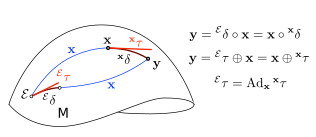
\includegraphics[width=0.7\textwidth]{figures/lie_group.pdf}
    \caption{Representations of a Lie group including the identity element $\cE$, operations of composition
    between increments and relations between a tangent space increment at the identity $\prescript{\cE}{}{\bftau}$ 
    and at the local element $\prescript{\bfx}{}{\bftau}$ through the adjoint matrix $\text{Ad}_{\bfx}$. Figure adapted from \cite{sola2018micro}.}
    \label{fig:lie_group} 
\end{figure}

\begin{figure}[h]
    \centering    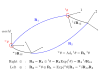
\includegraphics[width=0.7\textwidth]{figures/rotation_exp_log.pdf}
    \caption{Representation of $\SO(3)$ Lie groups operations. Note that we represented frames with different origins
    for better readability while the group elements only represent pure rotations (no translation). $world$ is the "global" reference 
    frame of the problem to which we assign the identity element of $\SO(3)$: $\bfI_3$. $1$ and $2$ are two frames of reference
    defined by their orientations \wrt $world$, $\Rot{}{1}$ and $\Rot{}{2}$. $\delta \Rot{}{12}$ is the relative rotation
    between elements $\Rot{}{1}$ and $\Rot{}{2}$ and can be computed using the exponential map on the angle axis $\bftheta$ expressed
    in $world$ or local frame, depending on whether we use the right or left $\oplus$ operator.}
    \label{fig:rotation_exp_log} 
\end{figure}

In robotics terms, $\prescript{1}{}{\bftheta}$ is the axis angle representation of the relative rotation $\prescript{1}{}{\delta \bfR}_{12} = \Rot{}{1}\tr\Rot{}{2}$ and
\textit{local} rotations represent the orientation of reference frames $\{1,2\}$ in a \textit{global} world reference frame. The identity element, therefore, corresponds 
to the world frame. 

Due to the general non-commutativity of the group operation, an additional $\oplus$ operator exists that retracts and composes vectors at the Lie algebra instead of
the local tangent space, the left-$\oplus$. The local operator, that corresponds to the manifold retraction, is called the right-$\oplus$. 
The Adjoint $\text{Ad}_{\bfx}\cM$ is an operator that maps elements from the local tangent space to the Lie algebra. 

\begin{equation}
    \prescript{\cE}{}{\bftau} = \text{Ad}_{\bfx}\cM \prescript{\bfx}{}{\bftau} 
\end{equation}

For rotation matrices, the adjoint matrix is $\text{Ad}_{\bfR}\SO(3)=\bfR$: to change the reference frame of the angle axis from local to global reference, it needs
to be rotated from one frame to another. Those operations are illustrated in \figRef{fig:rotation_exp_log}.


%
%
%
\section{Factor Graphs: a visual language for robotics estimation}
\label{sec:factor_graphs}

A crucial aspect of solving the MAP problem is the fact that the likelihood function is factorizable. This represents the fact that the problem
exhibits a particular structure that has important computational implications. We will first explain how this factorization can be described 
visually using a graphical model known as the \textit{Factor Graph} and then link this representation to the sparsity of the matrices involved
in solving the NLLS problem.


\subsection{Factor Graph representation}
Let us consider the toy example represented in \figRef{fig:toy_problem}. 
We wish to estimate the trajectory of a differential robot, that is its states at chosen timestamps called \textit{\keyframes}, and remarkable elements 
of the environment, called \textit{landmarks}. We suppose that this robot is equipped with an odometer, whose measurements integrated over time provide relative 
transformations between \keyframes, and an exteroceptive sensor that provides relative measurements between \keyframes~and landmarks.

\begin{figure}[h]
    \centering
    \begin{subfigure}{.49\linewidth}
        \centering
        \includegraphics[width=\textwidth]{figures/toy_example.pdf}
        \caption{\label{fig:toy_problem}}
    \end{subfigure}%
    \hfill
    \begin{subfigure}{.49\linewidth}
        \centering
        \includegraphics[width=\textwidth]{figures/toy_factor.pdf}
        \caption{\label{fig:toy_factor}}
    \end{subfigure}%
    \caption{(\subref{fig:toy_problem}): toy estimation problem, a differential drive robot equipped with an odometer moves in 
    an scene with landmarks represented by stars. (\subref{fig:toy_factor}): Factor Graph representation the problem, the estimated variables are represented by circles 
    (blue for robot \keyframes, green for landmarks) and factors by squares (orange for odometry, black for exteroceptive sensor, red for the prior).}
\end{figure}

In this case, the state variables are $\cX = \{ \bfx_1, \bfx_2, \bfx_3, l_1, l_2\}$  and measurements $\cZ = \{ z_{o,1}, z_{o,2}, z_{e,1}, z_{e,2}\}$.
We also apply a prior on the pose of the first \keyframe\ of the trajectory, which can be understood as fixing the frame origin of the reference 
frame in which the estimation is done.

The factorization of the likelihood of \eqRef{eq:likelihood_factorization} in this example writes:
%
\begin{align}
    p(\cX | \cZ) \propto 
    ~&{\color{Red} \phi_0({\color{Blue} \bfx_{0}})} \\ 
    ~&{\color{Orange} \phi_1({\color{Blue} \bfx_1}, {\color{Blue} \bfx_2}) \phi_2({\color{Blue} \bfx_2}, {\color{Blue} \bfx_3})} \\ 
    ~&{\color{Black} \phi_3({\color{Blue} \bfx_1}, {\color{Green} l_1}) \phi_4({\color{Blue} \bfx_2}, {\color{Green} l_1}, {\color{Green} l_2}) \phi_5({\color{Blue} \bfx_3}, {\color{Green} l_2})}
\end{align}

This factorization can be represented as a \textit{factor graph} as seen in \figRef{fig:toy_factor}. 
Factor graphs are popular probabilistic graphical models \cite{koller2009probabilistic} that can describe a vast family of statistical models \cite{loeliger2004introduction}.
In the general sense, a factor graph is a bipartite graph that represents the factorization of a function of several variables. In estimation , we use it to represent the factorized likelihood \eqRef{eq:factorized_likelihood}, or equivalently the NLLS problem \eqRef{eq:nlls_map_pbe}.

We adopt the visual notation commonly found in robotics: round nodes for variables, square nodes for factors, edges represent the dependency 
of each factor on a subset of variables. In the following parts, we will use the following terminology to designate factors depending on which variables they depend on:

\begin{itemize}
    \item \textbf{Unary factor} $\color{Red} \phi$: depends on a single \keyframes, obtained from a an absolute measurement (\eg a prior, GPS etc.)
    \item \textbf{Motion factor} $\color{Orange} \phi$: depends on successive \keyframes, obtained from a motion sensor (\eg wheel odometry, IMU etc.)
    \item \textbf{Relative} or \textbf{exteroceptive factor} $\phi$: depends on a \keyframe\ and a part of the map, a few landmarks in this case, obtained from exteroceptive sensors
\end{itemize}

Dellaert and Kaess \cite{dellaert2006square} were the first to
recognize the link between NLLS problems and factor graphs \cite{dong2019minisam}. Over the last two decades, they have grown in popularity among roboticists as a visual language to describe 
estimation problems \cite{dellaert2017factor} and planning problems \cite{dong2016motion}. As Frank Dellaert puts it \footnote{Citation from a recent talk,
see \href{https://www.youtube.com/watch?v=-yCC7mpgL4w}{this video}, around 15:30.}, factor graphs are "an amazing thing to write on blackboards".   
Aside from providing insights into the computational structure of the problems, they can be used as a common language between engineering teams
to convey insights about the nature of the problems to solve.

% The SLAM problem hereby represented as a factor graph in only one example of the vast family of estimation problems that can be modeled as a factor graph
% (other including \eg target tracking, structure-from-motion, control and planning \cite{}). 

The problems typically represented by factor graphs and found in estimation are very sparse.
Many specialized solvers \cite{grisetti2011g2o, kaess2012isam2, ila2017slam++} have been implemented to exploit this sparsity. 
Let us discuss the basis of sparse NLLS to conclude this chapter.
% A discussion of the particularities of factor-graph-based NNLS solvers can be found in \cite{dellaert2017factor, sola2017course}.




\subsection{Sparsity of the NLLS problem}

Each residual of the NLLS problem is a function of a small subset of the state variables. Therefore, each factor node in the Factor Graph representation of the problem is connected to but a few of the variable nodes. This makes for a graph with low connectivity. We will show that this low connectivity is linked to an important sparsity of the Jacobian matrix of the residuals.

The Jacobian matrix of the residuals $\bfJ \in \Reals^{M \times N}$ is a big sparse matrix of dimensions 
\begin{itemize}
    \item M rows = $\sum_{i=1}^{m}dim(\bfe_i) \rightarrow~$ the sum of residual dimensions
    \item N columns = $\sum_{i=1}^{n}dim(\cT_{\bfx_i}\cM_i)~\rightarrow$ the sum of variables tangent-spaces dimensions 
\end{itemize}   

Each block column corresponds to one of the state variables and each row corresponds to a residual. For each row, only the blocks corresponding to the
state variables that the residual depends on are non-zero. For instance, the matrix corresponding to the toy problem described in \figRef{fig:toy_problem} is:
\begin{equation}
    \bfJ=
    \begin{pmatrix}
        J^{0}_{\bfx_1} &   &     &     &     \\
       J^{o_1}_{\bfx_1} & J^{o_1}_{\bfx_2}  &     &     &     \\
                       & J^{o_2}_{\bfx_2}  & J^{o_2}_{\bfx_3}   &     &     \\
       J^{e_1}_{\bfx_1} &                  &     &  J^{o_2}_{\bfl_1}   &     \\
                       & J^{e_1}_{\bfx_2}  &     &  J^{e_1}_{\bfl_1}   &     \\
                       & J^{e_2}_{\bfx_2}  &     &     &  J^{e_2}_{\bfl_2}   \\
                       &                  & J^{e_3}_{\bfx_3}    &     &  J^{e_3}_{\bfl_2}   \\
    \end{pmatrix}
    \label{eq:sparse_jac}
\end{equation}



The approximate Hessian matrix $\bfH \in \Reals^{N \times N}$ displays a similarly remarkable sparsity that makes the resolution of the linear system
at each step very efficient. Algorithms such as the Schur complement \cite[A.5.5]{boyd2004convex}, Cholesky factorization \cite[C.3]{boyd2004convex}, 
and QR factorization \cite[C.5]{boyd2004convex} were applied by different authors to the problem of SLAM and estimation. 

\subsection{The algorithm (revisited)}
To tie things together, we now recapitulate the Gauss-Newton algorithm in the context of variables living on manifolds. 
We highlight the parts that differ from the regular Gauss-Newton algorithm with vector spaces.

\begin{enumerate}
    \item Initialize the state estimate at an initial value $\check{\cX} := \cX^0$ \\
    $\cX$ lives on a composite manifold. Its covariance is defined on the local tangent space of this manifold (see \secRef{sec:uncertainty_on_manifolds}).
    \item Approximate the NLLS cost function around the current estimate as a quadratic function \\
    The linear approximation is done using the notation of Jacobian on manifolds described in \secRef{sec:uncertainty_on_manifolds}.
    $\Delta \bfx$ is defined as the Cartesian representation of a composite tangent space element.  
    \item Find the optimal step $\Delta \bfx^*$ by solving a linear set of equations \eqRef{eq:linear_syst_GN} \\
    This part does not change. As mentioned in \secRef{sec:LM}, globalization of Gauss-Newton such as the Levenberg-Marquardt algorithm
    may alter the linear system to solved for increased performance.
    \item Update the current state estimate $\check{\cX} := \check{\cX} \oplus \Delta \bfx^*$ \\
    The update of the current state is done using the retraction operator $\oplus$ of the composite manifold \eqRef{eq:composite_retract}.
    \item Loop over steps 2-4 until convergence
\end{enumerate}

When the estimation algorithm has converged we can also obtain the covariance on the estimates (details and illustration are available in the 
appendix \chpRef{chp:MAP_covariance}). This is however a costly computation that is usually reserved for offline investigation of the estimation quality. 



\section{Conclusion}

We have described a general algorithm to solve NLLS problems with variables belonging to manifolds and weighted by covariance matrices. This problem
comes from framing the state estimation as a MAP problem and using multiple assumptions on the nature of the measurement models. These measurement models
are described as residuals weighted by their respective covariance matrices, representing the confidence we have in the sensor measurements. Factor Graphs can 
represent visually those problems and their connectivity is closely related to the sparsity of the linear problems appearing in the optimization algorithm.

In our opinion, two equally important research directions start from here: (i) finding new solvers extending these ideas to new sets of problems, such as multi-robot or multi-hypothesis problems, and (ii)
formulating new, efficient, and generalizable measurement models. This thesis mostly theoretically contributes to the direction of extending
the estimation model (ii) while we mostly rely on existing algorithms (i) to solve the subsequent problems.
A commonly used denomination in the context of robotics state estimation is to refer to the solver implementation as the \textit{backend} while the measurement models are referred to as \textit{front-ends}.

The next chapters each concentrate on a range of sensor modalities useful for legged robots:
object pose retrieval from vision algorithms, a generalized pre-integration theory for high rate sensors, legged robot kinematics, and the application 
of pre-integration to legged robots force measurements.






\chapter{Object level vision}
\minitoc


\section{General factor}
Let's assume that an algorithm provides us $\Tm{C}{O} \in \SE(3)$, a measurement the pose of an element 
of the scene with an attached frame $O$ with respect to the camera frame $C$ located at the Camera optical frame.
The kinematic chain of the problem described in \ref{fig:camera_object_chain} unrolls as 
$\T{W}{O} = \T{W}{B}\T{B}{C}\T{C}{O}$ where W and B correspond to the world and body frames.
Given measurement $\Tm{C}{O}$, this relation can therefore be turned into a residual relating 
the robot pose, the camera extrinsics and the object pose:

\begin{equation}
    \bfr (\T{W}{B}, \T{B}{C}, \T{W}{O}) = \Log(\T{W}{O} \T{W}{B}^{-1} \T{B}{C}^{-1} \T{C}{O}^{-1}) ~ \in \Reals^6
\end{equation}

We also assume that we have access to the covariance of this measurement 
$\Cov_V \in \Reals^{6 \times 6}$. We will now describe two applications of this factor, one using Apriltag fiducial markers and one using 
a Deeplearning object pose estimation algorithm.

\begin{figure}
    \centering
    \includegraphics[width=0.7\textwidth]{figures/fig_kinematic_Cesar.png}
    \caption{Camera/object kinematic chain from ICRA paper, to replace }
    \label{fig:camera_object_chain}
\end{figure}

\section{Fiducial marker}
\subsection{Markers Pose estimation algorithms}
Sota on the question
Apriltag: \cite{wang2016iros}
IPPE: \cite{collins2014infinitesimal}

\subsection{Covariance model}
Appart from designing more precise and more efficient algorithm for fiducial marker detection and specialized PnP algorithms,
 obtain covariances from these prediction has been the focus of a series of papers.
 SOTA

Instead of directly obtaining Jacobians from the PnP algorithms, we found that a natural way to proceed is to take the opposite 
direction. It should somehow be possible, knowing the marker size and the relative pose measurement, and assuming pixel noise, to
recover $\Cov_{OV}$. A simple model of this noise is to assume isotropic gaussian noise on the pixels. If we stack four pixel (the four tag corners) 
$\bfx_i = [u_i, v_i] \in \Reals^2$ and we stack then in the vector $\bfx = [\bfx_1 \bfx_2 \bfx_3 \bfx_4]$, we have therefore that
$\bfx$ is corrupted by a gaussian noise $\Cov_{\bfx} = \sigma_{x}^2 \bfI$, where $\sigma_{x}$ usually takes values of 1 or 2 pixels.
PnP algorithm provides us with a function $pnp$ defined as:

\begin{equation}
    \begin{split}
        f: \Reals^8 &\rightarrow SE(3) \\
                           \bfx &\rightarrow \T{C}{O} = pnp_w(\bfx)
    \end{split}
\end{equation}

where w denotes the dependency on the width of the marker. This $pnp_w$ function implementation depends on the specificities of the PnP algorithm used and  
is in general hard to differentiate. Instead if we consider the inverse function

\begin{equation}
    \begin{split}
        g: SE(3) &\rightarrow \Reals^8 \\
                           \T{C}{O} &\rightarrow \bfx = proj_w(\T{C}{O})
    \end{split}
\end{equation}

that maps the relative pose to the projection of the tag in the image, a rather simple jacobian expression can be derived using the chain rule, as follows.

Let's defined the marker corner coordinates in the marker frame, like shown in \fig \ref{fig:tag_coordinate_frame}:

\begin{equation}
    c =
    \begin{pmatrix}
    c_1 \\ c_2 \\ c_3 \\ c_4
    \end{pmatrix}
    ~~
    c_1 =  \begin{pmatrix} -1 \\ -1 \\ 0 \end{pmatrix}
    ~ 
    c_2 =  \begin{pmatrix} 1 \\ -1 \\ 0 \end{pmatrix}
    ~
    c_3 =  \begin{pmatrix} 1 \\ 1 \\ 0 \end{pmatrix}
    ~
    c_4 =  \begin{pmatrix} -1 \\ 1 \\ 0 \end{pmatrix}
\end{equation}
which coordinates have been rescaled by a factor $\frac{w}{2}$, that will be reintroduced later.

%
\begin{figure}
    \centering
    \includegraphics[width=0.4\textwidth]{figures/tag_coordinate_frame.png}
    \caption{Dummy tag image, annotate with coordinates }
    \label{fig:tag_coordinate_frame}
\end{figure}

Then, assuming that images are corrected (no distortion), the pinpoint camera model gives us that

\begin{equation}
    \bfx_i = eucl(h_i) = eucl(K\T{C}{O} c_i)
\end{equation}
for each corner $c_i$, where $h_i$ are the homogeneous coordinates representing the projected corners and $eucl$ is the euclideanization function defined as
\begin{equation}
    \begin{split}
        eucl: \Reals^3 &\rightarrow \Reals^2 \\
        h = \begin{pmatrix}x\\y\\z\end{pmatrix} &\rightarrow \bfx = \begin{pmatrix}x/z\\y/z\end{pmatrix}
    \end{split}
\end{equation}

We need to compute the jacobian of each corner projection with respect to the estimated relative pose $J^{x_i}_{\T{}{}} = J^{x_i}_{h_i} J^{h_i}_{\T{}{}}$. 
Regarding the transformation, we will consider it to be an element of $\Reals(3)\times \SO(3)$ since the translation and rotation part 
of transformation are treated separately in our solver. The expressions of those functions are therefore expressed as:

% DROP dependency on C L for clearer notation?
\begin{equation}
    \begin{split}
        &h_i = K(\Rot{C}{O}c_i + \posi{C}{O}) \\
        &J^{h_i}_{\posi{C}{O}} = K ~~~~~~ J^{h_i}_{\Rot{C}{O}} = -K\Rot{C}{O}[c_i]_{\times}  \\  
        &J^{h_i}_{\T{C}{O}} = [J^{h_i}_{\posi{C}{O}} ~J^{h_i}_{\Rot{C}{O}}] = K [I_3 ~~~ -\Rot{C}{O} [c_i]_{\times}]
    \end{split}
\end{equation}
while the euclideanization jacobian is found to be
\begin{equation}
    J^{x_i}_{h_i}
    =
    \begin{pmatrix}
    1/z_i & 0 & -x_i/z_i^2 \\
    0 & 1/z_i & -y_i/z_i^2
    \end{pmatrix}
\end{equation}


Finally, we can stack the 4 jacobians to get the full jacobian to be used for covariance propagation.
\begin{equation}
    J \triangleq J^{\bfx}_{\T{C}{O}}=
    \frac{w}{2}
    \begin{pmatrix}
    J^{\bfx_1}_{\T{C}{O}} \\ J^{\bfx_2}_{\T{C}{O}} \\ J^{\bfx_3}_{\T{C}{O}} \\ J^{\bfx_4}_{\T{C}{O}}
    \end{pmatrix}
    ~ \in \Reals^{8 \times 6}
\end{equation}
reintroduction the $\frac{w}{2}$ factor common to the 4 corners. 


We therefore have the covariance propagation equation $Q_{\bfx} = J Q_{\T{C}{O}} J^T$. 
This equation must be inverted in order to recover the needed covariance. $J$ being non square, 
we have to use the pseudo inverse to write: $\Cov_{\T{C}{O}} = J^{T,\dagger} \Cov_{\bfx} J^{\dagger}$. 
Knowing that the pixel noise covariance is isotropic as explained above, this equation simplifies to:

\begin{equation}
Q_{\T{C}{O}} = \sigma_{\bfx}^2(J^T J)^{-1}    
\end{equation}




\section{Object pose reconstruction}
\subsubsection{Cosypose}
Small sota + general cosypose workings
\subsubsection{Empirical covariance estimation}
blabla
\chapter{Kinematics}
\minitoc
\bigskip

The robot kinematic model along with encoder measurements make possible the computation of poses and spatial velocities \cite{featherstone2014rigid} (aka. twists) 
of reference frames attached to the robot segments relative to the base or world frame. This kinesthesis capability is of paramount importance to control
multi-body systems for locomotion or other interactions with its environment. If we have information about stable contacts that the robot keeps with
its environment, it is possible to infer a relative motion measurement, which is commonly called leg-odometry.

We will shortly describe the formulation of the forward kinematics algorithm, that enables to compute relative poses and spatial velocities between parts of the robot
and then show how this information can be used to define a leg-odometry factor to be added in the factor graph. The last section shows how forward kinematics can also be used to leverage prior 
information about the height of the environment. 



\section{Forward kinematics}
\label{sec:forward_kinematics}
We first describe the forward kinematics and differential kinematics algorithms by introducing notations commonly found in the legged robots literature.

The degrees of freedom (DoF) $n$ of a poly-articulated system is the minimal number of variables that completely describe his state given the base frame. 
For robots with rigid segments, the DoF of the robot is the sum of the DoFs of its joints (1 for linear and rotational joints, 3 for
ball joints, etc.).
The state of the joints (1 angle for rotational joints) can be stacked together in the vector of joint configurations 
$\qa \in \Reals^n$. For most simple joints, the joint configuration velocities are simply the time derivative $\dqa \in \Reals^n$\footnote{An exception is the ball joint where the 
state is defined as an element of $\SO(3)$, thus its velocity vector is defined as an angular velocity in $\Reals^3$.}. $\qa$ and $\dqa$ are typically obtained from
the joint encoder measurements.
Legged robots are not fixed to the ground so we add a so called "free-flyer" which is the pose of the base with respect to the world and is modeled as an unactuated joint of 6 DoF pertaining to the $\SE(3)$ group. Its velocities are therefore in the $\se(3)$  Lie algebra, isomorphic to $\Reals^6$. 

The whole body state of the robot is defined by the robot configuration vector $\bfq=[\bfq_b,\qa]\in \SE(3) \times \Reals^n$, where 

\begin{equation}
    \bfq_b \triangleq \T{W}{B} =  
    \begin{pmatrix}
        \Rot{W}{B} & \posi{W}{B} \\
        \bf0_3\tr & 1
    \end{pmatrix}
\end{equation}
%
is the configuration of the base,
with $\posi{w}{b} \in \Reals^3$ and $\Rot{W}{B} \in \SO(3)$ are the position and orientation of the base with respect to the world.
$\qa \in \Reals^n$ is the configuration of the joints. $\bfq$ therefore belongs to a composite manifold $\cM_{\bfq} = \left<\SE(3), \Reals^n \right>$ and the configuration velocity vector belongs to its tangent space $\se(3)\times \Reals^n$ which is isomorphic to $\Reals^{6+n}$: $\bfv_q \in \Reals^{6+n}$. Those are concatenations
of the base state and joint configuration vectors:
%
\begin{equation}
    \bfq= [\bfq_b, \qa]\in \cM_{\bfq}\quad\quad,
    \quad\quad
    \bfv_q= [\prescript{b}{}{\mathbf{\nu}}_b,\dqa]  \in \Reals^{6+n}
    \label{eq:configuration}
\end{equation}
%
where $\prescript{b}{}{\mathbf{\nu}}_b$ is the twist of the base frame expressed in the base frame.
The computation of any segment pose of index $k$ relative to the world is obtained using the forward kinematics (FK) algorithm:
%
\begin{equation}
    \T{W}{K} = \text{FK}_k(\bfq)
\end{equation}

The kinematic chains of most robots is can be represented as a tree whose root is the world frame, nodes are the joints to which are associated reference frames (including the base, which is considered as a $\SE(3)$ joint), and edges are solid segment placed between these nodes.
The forward kinematics algorithm consists in a forward pass from the root of the tree $\T{W}{B}$ through the joints along the path to the leaf $\T{W}{K}$ that we wish to obtain. Let us denote by $i$ the index of each intermediate joint between the root and the leaf, the root (world) having index 0 and the base index 1, the forward kinematics algorithm simply writes as a composition of successive transformations:

\begin{equation}
    \Tbar{0}{k} = \T{0}{1}(\bfq_b) \Tbar{1}{2'}
    \T{2'}{2}(q_2) \dots  \Tbar{k-1}{k'} \T{k'}{k}(q_k)
\end{equation}
%
where $\Tbar{i-1}{i'}$ designates the transformation between joint frames $i-1$ and $i$ when the joint configuration $q_i$ is at the identity value and is a constant. 
The $\T{i'}{i}(q_i)$ designate transformations caused by a non-zero joint value $q_i$, as reprsented in \figRef{fig:forward_kinematics}.

\begin{figure}
    \centering
    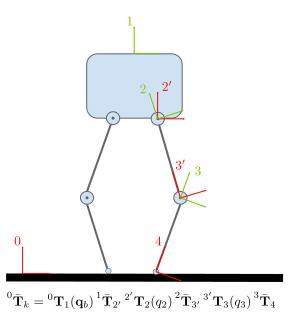
\includegraphics[width=0.5\textwidth]{figures/kinematic_tree_FK.pdf}
    \caption{Illustration of the Forward kinematics algorithm to get the transformation of the foot $4$ with respect to the world $0$.}
    \label{fig:forward_kinematics}
\end{figure}


It is also possible to obtain the pose relative to the base $\T{b}{k}$ by simply setting the base pose vector to be the identity pose $[0,0,0,~0,0,0,1]$.

% Differential FK is not used anywhere so...
% FK is a nonlinear function of the robot configuration. 
% To obtain the relative spatial velocity, we have to compute the jacobian $\bfJ_k$ of FK with respect to the configuration.
% The differential forward kinematics (DFK) is then simply:

% \begin{equation}
%     \prescript{w}{}{\mathbf{\nu}}_k = \bfJ_k \bfv_q    
% \end{equation}

Similarly, the spatial velocity relative to the base $\prescript{b}{}{\mathbf{\nu}}_k$ can be obtained by setting the base spatial velocity part of $\bfv_q$ to zero.
These algorithms are very fast to compute ($\approx 1\mu s)$ using modern dedicated libraries \cite{carpentier2019pinocchio}.

We will now see how FK can be used to derive leg odometry for a quadruped robot.

\section{Leg odometry}
We will restrict ourselves to the case of point feet as the main platform on which we experimented is a quadruped robot.
Quadrupeds are usually equipped with non-articulated round feet whose contact with the ground is, in first approximation, punctual.
Humanoid robots are equipped with articulated flat feet that provide richer information. In \secRef{sec:kinematic_info} we gave an exhaustive review of the types of leg 
odometry measurements that can be obtained on legged machines.

The basic idea is that we assume to have access to accurate contact detection. If the contact is held between time $t_i$ and $t_j$ and that
the contact point $L$ (to which a frame is attached) is fixed. This can be written $\posi{W}{L}^i = \posi{W}{L}^j$. 
In practice, the round feet of our robot can slightly roll but we will neglect this phenomenon for now. 
If we unfurl the transformation chain to make the base poses appear in the equation, we obtain the identity:

\begin{equation}
    \posi{}{}^i + \Rot{}{}^i \posim{B}{L}^i = \posi{}{}^j + \Rot{}{}^j \posim{B}{L}^j
\end{equation}

We can immediately derive the residual $\bfe^{LO}$ expression for each foot $l$ in contact between $t_i$ and $t_j$:

\begin{equation}
    \bfe^{LO}_l(\posi{}{}^i, \Rot{}{}^i, \posi{}{}^j, \Rot{}{}^j) = \posi{}{}^i + \Rot{}{}^i \posim{B}{L}^i - (\posi{}{}^j + \Rot{}{}^j \posim{B}{L}^j)
\end{equation}

To obtain a proper measurement model, we need to model the influence of measurement inaccuracies.
This equation depends on relative positions $\posim{B}{L}^i$ and $\posim{B}{L}^j$ that are computed using FK. The quality of the computation depends on several things:
the robot kinematic model (calibration), deviations from the rigid body model (\eg segment/joint flexibilities, backlash), encoder noise.
It is tempting to propagate encoder noise $\noise_{\qa}$ trough FK using the kinematic jacobian \cite{bloesch2013state, hartley2018legged}:

\begin{equation}
    \posim{B}{L} = FK(\qa + \noise_{\qa}) \approx FK(\qa) + \bfJ_L\noise_{\qa}, \quad \quad \Cov_{p} = \bfJ_L \Cov_{\qa} \bfJ_L
\end{equation}

However, the resolution of Solo encoder is actually very high: 0.002 degrees, which would account for a mere 10 \textit{micrometers} difference.
Therefore, most of the measurement errors come from the other mentioned effects. Unfortunately, those are much harder to model, and all act at the same time
in an unpredictable fashion. Thus, we opt for a simple additive noise on the foot position in the world:
%
\begin{equation}
    \posi{W}{L}^i = \posi{W}{L}^j + \noise_{LO}
\end{equation}
%
where $\noise_{LO} \sim \Gaussian{0}{\Cov_{LO}}$ denotes a Gaussian noise accounting for potential roll/slip of the foot and kinematic inaccuracies.
This noise can be modeled as white noise on the foot velocity $\noise_v$, which when integrated gives a random walk.  
Its variance after $\Dt$ is 
%
\begin{equation}
    \Cov_{LO} = \Dt \Cov_v
\end{equation}
%
where $\posim{B}{L}^i$ and $\posi{B}{L}^j$ are the contact positions in base frame at times $t_i$ and $t_j$ acquired from $\qa$ via forward kinematics. 
The residual errors $\bfe^{LO}_l$ and their covariances can be added as a factor to the factor graph that we wish to build.

In the literature review and \figRef{fig:kin_models}, this method is referred to as \textit{single foot matching}. To obtain
a relative transformation of the robot's base frame between $t_i$ and $t_j$, at least three stable feet contacts are necessary. When it is the case, it is possible to directly compute the
relative transformation, which would be integrated as a separate residual, by solving an orthogonal Procrustes problem \cite{roston1991dead}.

However, for trotting gates common for quadrupeds, the robot is most of the time standing on only two legs, which makes the Procrustes problem computation rarely applicable. Instead, we add a single factor for each foot in stable contact. In fact, when at least 3 feet are in stable contact, the information extracted from these combined factors is the same as if we had pre-computed a 6D transformation from the Procrustes problem. Besides, when fusing with other sensors (such as the IMU,
see \chpRef{chp:centroidal_estimation}), 1 or 2 legs in contact already provide sufficient information to make the desired variables observable.



\section{Terrain height}
If we only use leg odometry along with other sources of odometry such as an IMU (see \ref{chp:centroidal_estimation}, the position of the robot drifts after some time. However, if we have prior knowledge about the foot terrain height $h \in \Reals$, it is easy to define, for each foot $l$ in contact, the residual:

\begin{equation}
    \bfe^h_l(\posi{}{}, \Rot{}{}) = (\posi{}{} + \Rot{}{} \posi{b}{l})_z - h \quad, \quad e^{h}_l \in \Reals
\end{equation}

This residual can be assigned with a variance $\sigma_h^2$ which is hand-tuned. 
The error and its covariance form a unary factor (only depends on one \keyframe\ ) 
that can be added to the factor we want to build.
Giving information about the height of the feet of the robot grounds the robot base height estimates and cancels the accumulation of drift in the vertical direction.




\chapter{Preintegrated sensors}
\minitoc

\label{chp:preintegrated}

  
\section{A motivational example: IMU integration for graph optimization}
In this section we will introduce the IMU measurement model and explain why integrating these measurements in the world frame does not immediately
lead to a viable factor. We will then explain the observations that lead to the development of the IMU pre-integration algorithm by Lupton \cite{lupton-09}.

Let's consider the estimation of a robot base pose and velocity in the world frame. We will neglect effects due the rotation of the earth by assuming 
that our world frame (which is fixed wrt. the ground) is an inertial frame, which
is a common simplification in robotics scenarios \cite{forster2017-TRO}. Without loss of generality, we assume that the IMU frame is identical to the base frame 
in the following developments. Among available sensors, the IMU measurements are known to be noisy, biased, and affected by the gravity.

\begin{equation}
    \begin{split}
    \angvelm{}{} &= \angvel{B}{WB} + \bias_{\angvel{}{}} + \noise_{\angvel{}{}} 
    \\
    \accm{}{}    &= \Rot{B}{W} \grav + \acc{B}{WB} + \bias_{\acc{}{}} + \noise_{\acc{}{}} 
    \end{split}
    \label{eq:imu_meas_model}
\end{equation}
    
Other sensors can help estimate IMU biases so we include the biases in the estimator state.

\begin{equation}
    \bfx = [\posi{W}{WB}, \vel{W}{WB}, \Rot{W}{B}, \bias_{\bfa}, \bias_{\angvel{}{}}]
    \triangleq 
    [\bfp, \bfv, \Rot{}{}, \bias_{\bfa}, \bias_{\angvel{}{}}] 
\end{equation}

Once the IMU has been started, these biases slowly change over time, depending on the quality of the IMU used. This change is almost always modeled 
as a random walk which is close to the observed behavior for rather short periods of time \cite{hussen2015low}.
A dynamical model based on strapdown integration of IMU measurements can then be derived.
%
\begin{equation}
    \begin{split}
    \dot{\posi{}{}} = \vel{}{}  ~~~~~~~
    \dot{\vel{}{}} = \acc{W}{WB} ~~~~~~~
    \dot{\Rot{}{}} = \Rot{}{} [\angvel{B}{WB}]_{\times} ~~~~~~~
    \dot{\bias}_{\bfa} = \noise_{\bfa}  ~~~~~~~
    \dot{\bias}_{\angvel{}{}} = \noise_{\angvel{}{}} ~~~~~~~
    \end{split}
    \label{eq:imu_dyn_conti}
\end{equation}
%
Introducing the measurement equations \eqRef{eq:imu_meas_model} in continuous dynamics \eqRef{eq:imu_dyn_conti} and using a zero order hold
explicit Euler integration scheme during $\dt$ results in the discrete dynamics:

\begin{equation}
    \begin{split}
    \Rot{}{}^{k+1}  &= \Rot{}{}^{k}\Exp((\angvelm{}{}^k - \bias_{\angvel{}{}}^k - \noise_{\angvel{}{}}^k)\dt)
    \\
    \vel{}{}^{k+1}  &= \vel{}{}^{k} + \grav \dt + \Rot{}{}^{k}(\accm{}{}^k - \bias_{\acc{}{}}^k - \noise_{\acc{}{}}^k)\dt
    \\
    \posi{}{}^{k+1} &= \posi{}{}^{k} + \vel{}{}^{k}\dt + \frac{1}{2}\grav \dt^2 
    + \frac{1}{2}\Rot{}{}^{k}(\accm{}{}^k - \bias_{\acc{}{}}^k - \noise_{\acc{}{}}^k)\dt^2
    \end{split}
    \label{eq:imu_dyn_disc}
\end{equation}
    
Now, these equations relate variables variables between two state variables sampled at IMU frequency. To include these measurements in our smoothing estimator,
one solution would be to introduce new variables at the rate of the IMU. However, the size of the problem would grow very quickly. A better option
is to integrate IMU measurements during extended periods of time. If we simply integrate the sequence of IMU measurements $\cZ_{im}$ between timestamps 
$t_i$ and $t_m$ by unfurling \eqRef{eq:imu_dyn_disc}, we obtain:
%
\begin{equation}
    \begin{split}
    \Rot{}{}^{m}  &= \Rot{}{}^{i} \prod_{k=i}^{m} \Exp((\angvelm{}{}^k - \bias_{\angvel{}{}}^k - \noise_{\angvel{}{}}^k)\dt) \\
    \vel{}{}^{m}  &= \vel{}{}^{i} + \sum_{k=i}^{m} \Big[\grav \dt + \Rot{}{}^{k}(\accm{}{}^k - \bias_{\acc{}{}}^k - \noise_{\acc{}{}}^k)\dt \Big]  \\
    \posi{}{}^{m} &= \posi{}{}^{i} + \sum_{k=i}^{m} \Big[\vel{}{}^{k}\dt + \frac{1}{2}\grav \dt^2 
    + \frac{1}{2}\Rot{}{}^{k}(\accm{}{}^k - \bias_{\acc{}{}}^k - \noise_{\acc{}{}}^k)\dt^2 \Big]
    \end{split}
    \label{eq:IMUIntij}
\end{equation}
%
Assuming IMU biases stay constant during $\Dt^{im}$, 
\begin{equation*}
    \bias^i \triangleq [\bias_{\acc{}{}}^i, \bias_{\angvel{}{}}^i] \approx [\bias_{\acc{}{}}^k, \bias_{\angvel{}{}}^k]  ~~~ \forall k \in [i..m]
\end{equation*}
% \begin{equation*}
%     \bias_i \triangleq [\bias_{\acc{}{}i}, \bias_{\angvel{}{}i}] \approx [\bias_{\acc{}{}k}, \bias_{\angvel{}{}k}]  ~~~ \forall k \in [i..j]
% \end{equation*}
% \begin{equation*}
%     \bias_i \triangleq [\bias_{\acc{}{},i}, \bias_{\angvel{}{},i}] \approx [\bias_{\acc{}{},k}, \bias_{\angvel{}{},k}]  ~~~ \forall k \in [i..j]
% \end{equation*}
%
we could then directly derive a factor with an error between the expected delta $\hat\bfDelta_{im}$ and the measured delta $\bfDelta_{im}$ defined as:
% $e(\bfx^i, \bfx^j) = \bfDelta_{\bfx}(\bfx^i, \bfx^j)  \ominus  \bfDelta_{\cZ_{im}}(\bias^i, \bfx^i)$
%   where 
%
\begin{align}
    \hat\bfDelta_{im}(\bfx^i, \bfx^m) = 
    \begin{bmatrix}
    \Rot{}{}^{i,T} \Rot{}{}^{m}  \\
    \vel{}{}^{m}  - \vel{}{}^{i}  \\
    \posi{}{}^{m} - \posi{}{}^{i}
    \end{bmatrix}
\end{align}
%
and 
%
\begin{align}
    \bfDelta^{im}(\bias^i, \bfx_i) = 
    \begin{bmatrix}
    \prod_{k=i}^{m} \Exp((\angvelm{}{}^k - \bias_{\angvel{}{}}^i)\dt)  \\
    \sum_{k=i}^{m} \Big[\grav \dt + \Rot{}{}^{k}(\accm{}{}^k - \bias_{\acc{}{}}^i - \noise_{\acc{}{}}^k)\dt \Big]  \\
    \sum_{k=i}^{m} \Big[\vel{}{}^{k}\dt + \frac{1}{2}\grav \dt^2 
    + \frac{1}{2}\Rot{}{}^{k}(\accm{}{}^k - \bias_{\acc{}{}}^i)\dt^2 \Big]
    \end{bmatrix}
    \label{eq:IMUIntim}
\end{align}
%
Both quantities are recomputed at each evaluation of the residual by the nonlinear solver. $\bfDelta_{\bfx}(\bfx_i, \bfx_m)$ is fairly quick to compute.
However $\bfDelta_{\cZ_{im}}(\bias^i, \bfx_i)$ formulation requires to reintegrate the whole buffer of measurements which
is highly inefficient. This is due to the dependency on velocity, orientation and biases at timestamp $i$. However the terms of equation \eqRef{eq:IMUIntij} can 
be rearranged (proof in the annex \secRef{sec:forster_proof}) to give:
%
% WITH NOISE
% \begin{equation}
%     \begin{split}
%     \bfDelta \Rot{}{im} &\triangleq  \Rot{}{}^{i,T} \Rot{}{}^{m} =  \prod_{k=i}^{m} \Exp((\angvelm{}{}^k - \bias_{\angvel{}{}^k} - \noise_{\angvel{}{}^k})\dt) \\
%     \bfDelta \vel{}{im} &\triangleq \Rot{}{}^{i,T} (\vel{}{j} - \vel{}{i} - g \Dt^{im}) 
%     = \prod_{k=i}^{m} \bfDelta \Rot{}{ik} \Exp((\accm{}{}^k - \bias_{\acc{}{}}^k - \noise_{\acc{}{}}^k)\dt)  \\
%     \bfDelta \posi{}{im} &\triangleq \Rot{}{}^{i,T}(\posi{}{}^j - \posi{}{}^i - \vel{}{}^i \Dt^{im} - \frac{1}{2} \grav \Dt^{im}^2) 
%     = \sum_{k=i}^{m} \Big[\bfDelta \vel{}{ik}\dt +  \frac{1}{2} \bfDelta \Rot{}{ik} (\accm{}{}^k - \bias_{\acc{}{}}^k - \noise_{\acc{}{}}^k)\dt^2 \Big]
%     \end{split}
%     \label{eq:IMUPreintij}
% \end{equation}
%
\begin{equation}
    \begin{split}
    \DR^{im} &\triangleq  \Rot{}{}^{i,T} \Rot{}{}^{m} \\
             &=  \prod_{k=i}^{m} \Exp((\angvelm{}{}^k - \bias_{\angvel{}{}}^i)\dt) \\
    \Dv^{im} &\triangleq \Rot{}{}^{i,T} (\vel{}{m} - \vel{}{i} - \grav \Dt^{im}) \\
             &= \prod_{k=i}^{m} \DR^{ik} \Exp((\accm{}{}^k - \bias_{\acc{}{}}^i)\dt)  \\
    \Dp^{im} &\triangleq \Rot{}{}^{i,T}(\posi{}{}^m - \posi{}{}^i - \vel{}{}^i \Dt^{im} - \frac{1}{2} \grav \Dt^{im,2}) \\
             &= \sum_{k=i}^{m} \Big[\Dv^{ik}\dt +  \frac{1}{2} \DR^{ik} (\accm{}{}^k - \bias_{\acc{}{}}^i)\dt^2 \Big]
    \end{split}
    \label{eq:IMUPreintij}
\end{equation}
%
where we define $\DR^{ik} \triangleq \Rot{}{i,T} \Rot{}{}^k$.
We then overwrites our delta notations as $\bfDelta_{\bfx,im}(\bfx_i, \bfx_m) = \bfDelta_{\cZ_{im}}(\bias^i)$
which lifts the dependency of the right hand term on the initial state $\bfx_i$. However the bias terms in \eqRef{eq:IMUPreintij} still enforce the repeated 
reintegration of the measurements buffer. Instead, the right hand side can be integrated once using biases estimates at the time where we begin to integrate them that
we note $\biasbar_i$. Then, we can approximate changes due to the newly estimated bias $\bias_i$ using a first order approximation.
% $\bfDelta_{\cZ_{im}}(\bias^i) = \bar{\bfDelta}_{\cZ_{im}} \oplus (\bfJ^{\bfDelta_{\cZ_{im}}}_{\bias_i} (\bias^i - \biasbar^i))$.

These two observations were first made by Lupton \cite{lupton-09}, whose formulation relied on Euler angles, and were later formalized on \SO(3) using Lie theory
by Forster \cite{forster2017-TRO}. The above equations are not directly useful for the implementation of pre-integration. We need first to derive a recursive formulation 
of the problem. IMU noise propagation also needs to be described in order to obtain covariances associated to the factor error. In the next section, we will take 
a step back and derive a pre-integration generalized to other proprioceptive sensors.



\section{Generalized pre-integration}
\label{sec:general-preint}


Pre-integration refers to the integration of high rate proprioceptive sensory data in an efficient way in the context of factor graphs. 
It was initially developed to deal with IMU measurements \cite{lupton-09, forster2017-TRO}. 
As we have seen, if a standard integration is conducted naively to derive a factor measurement between two KFs, 
then the IMU data needs to be reintegrated at each solver iteration because the integral depends on the states we are to estimate. 
The IMU pre-integration theory solves this issue and can be generalized to any proprioceptive sensor as shown in \cite{atchuthan-18-thesis,deray-19-selfcalib,fourmy2021contact}. 
Delta quantities $\bfDelta_{im}$  are defined between KFs $i$ and $m$ so that $\bfx_m=\bfx_i\boxplus\bfDelta_{im}$. A suitable composition $\boxplus$ is chosen so that $\bfDelta_{im}$ 
does not depend on the initial states $\bfx_i$. 
Dependence on other small-varying parameters $\bfb$ such as sensor bias is linearized as $\bfDelta_{im}(\bfb)=\bfDelta_{im}(\ol\bfb)\op\bfJ^\bfDelta_\bfb(\bfb-\ol\bfb)$.
Then we can pre-integrate $\ol\bfDelta_{im}\te\bfDelta_{im}(\ol\bfb)$ once during data gathering, and use it to define residuals that are later evaluated many times by the optimizer.
This was the main contribution of paper my paper \cite{fourmy2021contact}.

\subsection{Delta pre-integration}

\begin{figure}[tb]
    \centering
    \includegraphics[width=0.6\textwidth]{figures/delta_time}
    \caption{
    The pre-integrated delta $\bfDelta_{ij}$ contains all motion from the last KF at time $i$, up to time $j$. 
    The current delta $\bfdelta_k$ contains the motion from times $j$ to $k$, computed from the last IMU measurement at time $k$.}
    \label{fig:delta_time}
\end{figure}

We perform pre-integration incrementally as follows. 
First, $\ol\bfDelta_{ii}$ is initialized to the null motion. 
Its covariance $\bfSigma_\Delta^{ii}$ and the Jacobian $\mjac{\bm\delta_i}{\bfb_i}$ are set to zero. 
At each reception of sensor data $\tilde\bfz_k$ at $t_k$, we integrate during $\dt$ to obtain the delta corresponding to a single data sample
%
\begin{align}
\bm\delta_k = f(\tilde\bfz_k, \ol\bfb_i, \dt)~, 
\label{eq:data2delta}
\end{align}

using the bias $\ol\bfb_i$ available in KF $i$. 
This single delta is integrated onto the delta pre-integrated so far using the delta composition law

\begin{align}
\ol\bfDelta_{ik} = \ol\bfDelta_{ij} \circ \bm\delta_k~. 
\label{eq:deltaPlusDelta}
\end{align}

which is represented in figure \figRef{fig:delta_time}.
%with Jacobians $\mjac{\ol\bfDelta_{ik}}{\ol\bfDelta_{ij}}$ and $\mjac{\ol\bfDelta_{ik}}{\bm\delta_k}$. 
The Jacobian of the pre-integrated delta with respect to biases, as well as the delta covariance, are also pre-integrated

\begin{align}
    \mjac{\bfDelta_{ik}}{\bfb_i} &= \mjac{\bfDelta_{ik}}{\bfDelta_{ij}}\mjac{\bfDelta_{ij}}{\bfb_i} 
+ \mjac{\bfDelta_{ik}}{\bm\delta_k}\mjac{\bm\delta_k}{\bfb_i} \\
    \bfSigma_\Delta^{ik} &= \mjac{\bfDelta_{ik}}{\bfDelta_{ij}}\bfSigma_\Delta^{ij}\mjac{\bfDelta_{ik}}{\bfDelta_{ij}}\tr 
+ \mjac{\bfDelta_{ik}}{\bm\delta_k}\mjac{\bm\delta_k}{\bfz_k}\bfSigma_\bfz\mjac{\bm\delta_k}{\bfz_k}\tr\mjac{\bfDelta_{ik}}{\bm\delta_k}\tr
\end{align}

where $\mjac{\bm\delta_k}{\bfb_i}$, $\mjac{\bm\delta_k}{\bfz_k}$, $\mjac{\bfDelta_{ik}}{\bfDelta_{ij}}$ and $\mjac{\bfDelta_{ik}}{\bm\delta_k}$ 
are the Jacobians $\mjac{y}{x}=\partial y/\partial x$ of (\eqRef{eq:data2delta},\eqRef{eq:deltaPlusDelta}), computed according to Lie theory \cite{sola2018micro}.


\subsection{Residual definition}
\label{sec:preint_residual}

The pre-integrated $\ol\bfDelta_{im}$ is used at the end of the pre-integration to define the residual

\begin{align}
    \bfr_{im} = (\ol\bfDelta_{im} \oplus \mjac{\bfDelta_{im}}{\bfb_i}(\bfb_i-\ol\bfb_i) ) \ominus \hat\bfDelta_{im}
    \label{eq:preint_residual}
\end{align}

where $\bfb_i$ is the current bias value,  $\hat\bfDelta_{im}=\bfx^m\boxminus\bfx^i$ is the expected delta between KFs, and $\{\op,\om\}$ are the composite
 plus and minus operators described in \cite{sola2018micro}. 
That is, $\{\op,\om\}$ are $\{+,-\}$ for vectors, and for rotations we have $\bfR\op\bm\theta\te\bfR\Exp(\bm\theta)$ and $\bfR_2\om\bfR_1\te\Log(\bfR_1\tr\bfR_2)$. 
The residual clearly depends on the KF states $\bfx^i,\bfx^m$ and the bias $\bfb_i$. It has an associated covariance  $\bfSigma_\Delta^{im}$.



\subsection{IMU pre-integration}

The states involved in this integration are the base states $\bfx_b = [\posi{}{}, \bfv, \Rot{}{}]$ with deltas $\bfDelta=[\Dp,\Dv,\DR]$. 
The IMU produces biased and noisy measurements $\tilde\bfz = [\tilde\bfa, \tilde{\bfomega}]$ of the base proper acceleration and angular velocity, 
with bias $\bfb = [\bias_{a}, \bias_{\omega}]$ and noise $\noise = [\noise_{a}, \noise_{\omega}]$. 

The pre-integration method in  \cite{forster2017-TRO} can be put in the formalism above by realizing that defining $\bm\delta=f(\tilde\bfz,\bfb,\dt)$ in \eqRef{eq:data2delta} as

\begin{align}
    \bm\delta^k = \begin{bmatrix}
    \delta\bfp\\\delta\bfv\\\delta\bfR
    \end{bmatrix}^k =
    \begin{bmatrix}
    \tfrac12(\tilde\bfa-\bfb_a-\noise_a)\dt^2 \\
    (\tilde\bfa-\bfb_a-\noise_a)\dt \\
    \Exp((\tilde{\bfomega}-\bfb_\omega-\noise_\omega)\dt)
    \end{bmatrix}^k
\end{align}

and the composition law $\bfDelta^{ik}=\bfDelta^{ij}\circ\bm\delta^k$ in \eqRef{eq:deltaPlusDelta} as

\begin{align} \label{eq:composition_delta}
    \begin{split}
    \Dp^{ik} 
    &= \Dp^{ij} + \Dv^{ij}\dt + \DR^{ij}\dpp^{k} \\
    \Dv_{ik} 
    &= \Dv^{ij} + \DR^{ij}\dv^{k} \\
    \DR^{ik} 
    &= \DR^{ij}\dR^{k} 
    \end{split}
\end{align}

then $\bfx_k=\bfx_i\boxplus\bfDelta_{ik}$ is \cite[eq.~32]{forster2017-TRO} and $\bfDelta_{ik}=\bfx_k\boxminus\bfx_i$ is \cite[eq.~33]{forster2017-TRO}. 
Full details can be found in \cite[Section 3.4]{atchuthan-18-thesis}.



%
%
%
%
\section{IMU pre-integration on Lie groups}
In \cite{fourmy2019absolute}, we showed that an alternative formulation of IMU preintegration on Lie groups was possible.
We introduce a new matrix Lie group representation of
the IMU deltas. The complete IMU pre-integration theory,
including the computation of the residual, is based on this
new Lie structure. The theoretical material for the Lie
development in this section can be found in the report \cite{sola2018micro}.


\subsection{Lie Group formulation}

We propose a matrix form of the Lie group of IMU deltas as,
%
\begin{align}\label{equ:delta_Lie}
\D &= 
\begin{bmatrix}
\DR & \Dv & \Dp \\
\bf0 & 1 & \Dt \\
\bf0 & 0 & 1
\end{bmatrix} \in \cD \subset \bbR^{5\times 5}
~.
\end{align}

Group identity, inverse and composition stem from regular matrix identity, inverse (with $\DR\inv=\DR\tr$) and product,

\begin{align}
\D_\cE&=\begin{bmatrix}
\bfI & \bf0 & \bf0 \\
\bf0 & 1 & 0 \\
\bf0 & 0 & 1 
\end{bmatrix} = \bfI_{5\times5}
\label{equ:identity}
\\
\D\inv &= \begin{bmatrix}
\DR\tr & -\DR\tr\Dv & -\DR\tr(\Dp-\Dv\Dt) \\
\bf0 & 1 & -\Dt \\
\bf0 & 0 & 1
\end{bmatrix} 
\label{equ:inverse}
\\
\D\cdot\bm\delta 
&= 
\begin{bmatrix}
\DR\dR & \Dv + \DR\dv & \Dp+\Dv\dt + \DR\dpp \\
\bf0 & 1 & \Dt+\dt \\
\bf0 & 0 & 1
\end{bmatrix}
~.
\label{equ:composition}
\end{align}
%
% Comparing against \eqsRef{equ:composite_identity}{equ:composite_composition} we observe that this matrix Lie group is exactly equivalent to the classical IMU deltas above.



\subsubsection{Lie algebra \texorpdfstring{$\mathfrak{d}$}{d} and exponential map}

The Lie algebra elements $\bftau\hhat$ and their isomorphic Cartesian $\bftau$ have the forms
%
\begin{align}\label{equ:lie_algebra}
    \bftau\hhat &= \begin{bmatrix}
    \hatx{\bth} & \bfrho & \bfupsilon \\
    \bf0 & 0 & \Dt \\
    \bf0 & 0 & 0
    \end{bmatrix} \in \mathfrak{d}
    ,&
    \bftau &= \begin{bmatrix}
    \bfrho \\ \bfupsilon \\ \bth \\ \Dt
    \end{bmatrix}
    \te \begin{bmatrix}
    \bfv\Dt \\ \bfa\Dt \\ \bw\Dt \\ \Dt
    \end{bmatrix} 
    \in \bbR^{10}
    ,
\end{align}
%
with $\bfv\te\dot\Dp$, $\bfa\te\dot\Dv$ and $\hatx{\bw}\te\DR\tr\dot\DR$.
Operators $\wedge$ and $\vee$ are defined so that $\bftau\hhat=(\bftau)\hhat$ and $\bftau=(\bftau\hhat)\vvee$.

The exponential map transfers tangent elements to the group; the logarithmic map is its inverse,
%
\begin{align}
    \D &= \Exp(\bftau) \te \exp(\bftau\hhat) = \begin{bmatrix}
    \Exp(\bth) & \bfQ\bfupsilon & \bfQ\bfrho+\bfP\bfupsilon\Dt \\
    \bf0 & 1 & \Dt \\
    \bf0 & 0 & 1
    \end{bmatrix} %\in\cD 
    \label{equ:exp}
    \\
    \bftau &= \Log(\D) \te \log(\D)\vvee = \begin{bmatrix}
    \bfQ\inv(\Dp-\bfP\bfQ\inv\Dv\Dt) \\
    \bfQ\inv\Dv \\
    \Log(\DR) \\
    \Dt 
    \end{bmatrix} %\in \bbR^{10}
    \label{equ:log}
\end{align}
%
where $\Log()$ is obtained by identifying terms in \eqRef{equ:delta_Lie} and \eqRef{equ:exp}.
Matrices $\bfP$ and $\bfQ$ are provided in the appendix \ref{sec:IMULieGroup}.


\subsubsection{Jacobians, uncertainty}
\label{sec:uncertainty}

For general functions $f:\cM\to\cN;y=f(x)$, we propagate uncertainty normally via the Jacobians $\mjac{y}{x}\te\dpar{y}{x}$, \ie, $\bfSigma_y=\mjac{y}{x}\,\bfSigma_x\,\mjac{y}{x}\tr$. 
These Jacobians map the tangent spaces of the mannifolds $\cM,\cN$ at $x$ and $y$, and in case of vector spaces they resort to the classical Jacobian.
They also satisfy the chain rule, which we use extensively in our developments.
We provide ample reference and justification of this approach in the technical report \cite{sola2018micro}.

A comment is however necessary for the present IMU case.
It relates to the uncertainty of the last component of the tangent space \eqRef{equ:lie_algebra}, which is the time $\Dt$. This component has no uncertainty by definition. 
Having it in the covariances would imply singularity and result in the risk of a number of well-known numerical issues. 
We therefore systematically marginalize this time component out of the covariances, simply by removing the last row and column. 



\subsubsection{Delta Lie group IMU factor residual}
Computation of the residual in the case of the Lie Delta group formulation follows the steps defined in \secRef{sec:general-preint}.
However, since the Delta is directly defined as a Lie group, the formulation is actually simplified because  ... 
Use the pre-integrated Jacobian $\mjac{\D_{im}}{\bfb}$ to correct the pre-integrated delta $\ol\D_{im}$ to account for the new bias estimate $\bfb_i\neq\ol\bfb_i$,

\begin{align}
    \D_{im}(\bfb_i) &= \ol\D_{im}\cdot\Exp(\mjac{\D_{im}}{\bfb}(\bfb_i-\ol\bfb_i)) 
    ~.
\end{align}

Use [Forster delta def] \eqRef{equ:delta} as $\boxminus$ to compute the expected delta from  $\bfx_i$ to $\bfx_m$,

\begin{align}
    \widehat\D_{im}(\bfx_i,\bfx_m) &= \bfx_m \boxminus \bfx_i 
    ~.
\end{align}
Compute the residual in the  tangent of $\cD$ at $\D_{im}$,

\begin{align}
    \bfr^\Delta_{im}(\bfx_i,\bfx_m,\bfb_i) &= \Log(\D_{im}(\bfb_i)\inv \cdot \widehat\D_{im}(\bfx_i,\bfx_m)) \in \bbR^9
~,
\end{align}

and drop the $\Dt$ part from the residual after the $\Log()$ ---see comment in \secRef{sec:uncertainty}.
In this last equation, the composite minus operator $\oplus$ is simply the traditional Lie group "minus" operator defined in [cite sola eq ...] applied
between the corrected preintegration delta and the expected delta.



\subsection{IMU Lie group versus Forster's method}

Mathematically, and disregarding methodology, the main difference between our method and Forster's \cite{forster2017-TRO} is to be found in the exponential map. 
To see it, let us consider small rotation increments $\bth=\bw\dt$ captured at each single IMU sample. 
In such cases, the matrices $\bfP,\bfQ$ appearing in the exponential map \eqRef{equ:exp} and detailed in \eqRef{equ:RQP} can be approximated by $\bfP\approx\tfrac12\bfI$ and $\bfQ\approx\bfI$.
The exponential becomes,
%
\begin{align}
    \Exp\left(\begin{bmatrix}
    \bf0 \\ \bfa \\ \bw \\ 1
    \end{bmatrix}\dt\right) \approx \begin{bmatrix}
    \Exp(\bw\dt) & \bfa\dt & \tfrac12\bfa\dt^2 \\
    \bf0 & 1 & \dt \\
    \bf0 & 0 & 1
    \end{bmatrix}
~,
\end{align}
%
where we find the terms $\bfa\dt$ and $\tfrac12\bfa\dt^2$, which should sound familiar from Forster's method. 
In effect, with this approximation, if we now compact all the steps \eqsRef{equ:pre_calibration}{equ:pre_composition} of our integration into a cumulative expression,
%
\begin{align}
    \D_{ik} = \prod_{j=i+1}^k \Exp\left(\begin{bmatrix}
    \bf0 \\ (\bfa_j-\bfa_{bi}) \\ (\bw_j-\bw_{bi}) \\ 1
    \end{bmatrix}\dt\right)
~,
\end{align}
%
it is possible (although tedious) to show that both Forster's and our method are exactly equivalent when $\bw\dt\to0$.
% , which is usually a valid hypothesis.
% These differences should not constitute an argument against Forster, since in practice we typically have extremely small steps $\bw\dt$ and the approximation holds very well.





\section{External force pre-integration}
In this section we apply the generalized pre-integration algorithm to the problem of using measured external
forces applied on a legged robot in a smoothing estimator. We propose to integrate the underactuated that we first recall. Then 
we derive the specificities of the pre-integration of external forces of a poly-articulated system. This is the main theoretical contribution
of our paper \cite{fourmy2021contact}.


\subsection{Centroidal dynamics}
\label{sec:centroidal_dynamics}
The robot dynamics is described by the well-known:
\begin{equation}\label{eq:wbdyn}
  \bfM(\q) \vq + h(\q,\vq) = \bm\tau_q + \sum_l \bfJ_l\tr \bff_l
\end{equation}
where $\q,\vq,\dvq,\bm\tau_q$ are the position, velocity, acceleration and torques of the robot in configuration space,
$\bff_l$ are the contact forces (written as 3D forces in this paper),
$\bfM$ is the generalized inertia matrix, $h$ the sum of gravity, Coriolis and centrifugal forces, and $\bfJ_l$ the jacobians of the contact points.
Because of the underactuated nature of legged robots, the configuration is often separated into $\q=(\posi{W}{B},\Rot{W}{B},\qa)$ where $\posi{W}{B}$ 
is the position in world frame of the robot base (typically, the torso or in our case the IMU), $\Rot{W}{B}$ the rotation of the base body with respect 
to the world and $\qa$ are the joint configuration of the actuated joints. 
%We will subsequently use the notation $\prescript{X}{}{[\cdot]}_Y$ to denote vectorial quantities of frame $Y$ expressed in frame $X$. A tilde $\Tilde{[\cdot]}$ denotes a noisy measurement.

While~\eqRef{eq:wbdyn} represents the whole dynamics, a subpart of it is of particular importance for legged robots.
The centroidal dynamics is written by the two equations:
%
\begin{equation}
    m \ddot{\bfc} = m \bfg + \sum_l \bff_l \quad , \quad
\dAM = \sum_l (\posi{}{l} - \COM) \times \bff_l
\label{eq:NewtonEuler}
\end{equation}
%
where $\COM,\AM$ are the position of the Center of Mass (CoM) and Angular Momentum (AM) around the CoM (both expressed in world frame), $m$ is the robot total mass, 
and the $\posi{}{l}$ are the positions of the contact points in world frame. The centroidal dynamics is an exact part of \eqRef{eq:wbdyn} and more deeply reveals 
the underactuation: the robot can move only if applying the proper forces to the environment, as the joint torques alone cannot lead to any modification 
of CoM or AM.


The classical approach in estimation of legged robot state is to first estimate the base state, and then to reconstruct the centroidal state $(\bfc,\dot{\bfc},\AM)$ using the joint position and velocity measurements, and the robot model.
This assumes that there is no direct measurement of the centroidal state.
Consequently, we are not be able to recover the exact centroidal state if there is any bias in the robot model.

Yet, we can see from the centroidal dynamics that the force measurements are connected to the variation of the centroidal state.
As observed in~\cite{carpentier2016center}, a proper fusion of the force measurements with an estimation of the state of the base makes the centroidal state observable.


\subsection{Force pre-integration factor}

The Newton-Euler equations \eqRef{eq:NewtonEuler} relate the evolution of the CoM and AM due to gravity, external forces and torques. 
In the case of a legged robot with punctual contact feet, only forces $\forcem{}{L}$ are applied at each limb contact $L$, with no torque. 
We assume that at each  limb contact we have access to noisy local force measurements $\forcem{}{L} = \force{L}{L} + \noise_f$. 
To transform them into the body frame $b$, we compute $\Rotm{}{L} \triangleq \Rot{B}{L}(\qa)  \in SO(3)$ and $\posim{}{L} \triangleq \posi{B}{L}(\qa) \in \Reals^3 $ from the joint configuration $\qa  \in \Reals^{12}$. 
The lever arm $(\posi{}{L}-\bias_c)$ in \eqRef{eq:NewtonEuler} uses a measurement of the CoM position in base frame $ \posi{B}{C}(\qa) \in \Reals^3$. 
This measure is biased due to inaccuracies in the robot model and therefore we add a bias variable to be estimated, $\bias_c \in \Reals^3$ so that $\posim{}{C} = \posi{B}{C}(\qa) + \bias_c + \noise_c$.
Assuming constant forces during each interval $\dt$ 
the integration of \eqRef{eq:NewtonEuler} yields the discrete dynamic model for the centroidal states:
%
\begin{equation}
\begin{split}
\COM^{k} &= \COM^{k-1} + \COMd^{k-1} \dt+\frac{1}{2} \bfg \dt^2 + \frac{1}{2m} \Rot{}{}^{k-1} \sum_L \Rotm{}{L}^k (\forcem{}{L}^k - \noise_{f}) \dt^2
\\
\COMd^{k}&= \COMd^{k-1} + \bfg \dt + \frac{1}{m} \Rot{}{}^k \sum_L\Rotm{}{L}^k (\forcem{}{L}^k - \noise_{f}) \dt 
\\
\AM^{k} &= \AM^{k-1} +\Rot{}{}^k \sum_L (\posim{}{L}^k  - \posim{}{C}^k +  \bias_{c}^k + \noise_{c}) \times \Rotm{}{L}^k(\forcem{}{L}^k - \noise_{f}) \dt
\end{split}
\label{eq:COMDiscrete}
\end{equation}
%
Analogously to the IMU case, it is possible to pre-integrate force measurements to derive a factor on the states 
$\bfx_c=[\COM, \COMd, \AM, \Rot{}{}]$ using deltas $\D_c=[\D\COM, \D\COMd, \D\AM, \DR]$. 
The rotation measured by the gyroscope has to be included too for the pre-integration to work. 
In this case, the bias vector is $\bias = [\bias_c, \bias_{\omega}]$. We define measurements  $\bfz^k$ to be:
%
\begin{equation}
\bfz^k = \left[ \posim{}{C}^k, \angvelm{}{}^k, \left[\forcem{}{L}^k, \posim{}{L}^k, \Rotm{}{L}^k \right]_{L=1..4}\right]
\end{equation}

The following operators are enough to particularize the  method in \secRef{sec:general-preint} to the contact forces case.
Integrating $\bfz_k$ during $\dt$ yields $\bm\delta_k$ in \eqRef{eq:data2delta} as
%
\begin{equation}
\small
    \bm\delta^{k}(\bfz^k, \bfb^i, \dt) =
    \begin{bmatrix}
    \frac{1}{2m} \sum_l \Rotm{}{L}^k \forcem{}{L}^k \dt^2
    \\
    \frac{1}{m} \sum_l \Rotm{}{L}^k \forcem{}{L}^k \dt 
    \\
    (\sum_l \posim{}{L}^k - (\posim{}{C}^k - \bias_c^i) \times (\Rotm{}{L}^k \forcem{}{L}^k ))\dt
    \\
    \Exp((\angvelm{}{}^k - \bias_{\omega}^i)\dt)
    \end{bmatrix}
\normalsize
\end{equation}
%
and the delta composition law in \eqRef{eq:deltaPlusDelta} as
%
\begin{equation}
    \D \circ \bm\delta = 
    \begin{bmatrix}
    \D\COM + \D\COMd \dt + \DR  \delta\COM
    \\
    \D\COMd + \DR  \delta \COMd
    \\
    \D\AM + \DR  \delta \AM
    \\
    \DR\dR
    \end{bmatrix}
    ~.
    \label{eq:DeltaDTCompo}
\end{equation}
%
The expected delta $\D^{ik}=\bfx^k\boxminus\bfx^i$ between KFs $i$ and $k$ reads
%
\begin{equation}
\D^{ik} =
\begin{bmatrix}
   \D\COM^{ik} \\ \D\COMd^{ik} \\ \D\AM^{ik} \\ \DR^{ik}
\end{bmatrix}
=
\begin{bmatrix}
	{\Rot{}{}^i}\tr (\COM^k - \COM^i - \COMd^i \Dt^{ik})
	\\
	{\Rot{}{}^i}\tr (\COMd^{k} - \COMd^{i} - \bfg \Dt^{ik})
	\\
	{\Rot{}{}^i}\tr (\AM^{k} - \AM^{i})
	\\
    {\Rot{}{}^i}\tr \Rot{}{}^k
\end{bmatrix}
~.
\end{equation}
%
Finally, the propagation of the state $\bfx_i$ to $\bfx_k$ using $\D_{ik}$, which can be used to retrieve a state at any time $k$ between KFs in the trajectory, is
%
\begin{equation}
	\bfx^k = \bfx^i \boxplus \D^{ik} =
	\begin{bmatrix}
	\COM^i + \COMd^i \Dt^{ik} + \Rot{}{}^i \Delta \COM^{ik} + \frac{1}{2} \bfg \Dt^{ik,2}
	\\
	\COMd^i + \Rot{}{}^i \Delta \COMd^{ik} + \grav \Dt^{ik}
	\\
	\AM^i + \Rot{}{}^i \Delta \AM^{ik}
	\\
	\Rot{}{}^i \DR^{ik}
	\end{bmatrix}
\end{equation}
%
%
%
%


\section{Related works}

Pre-integration principles were first proposed by Lupton \cite{lupton-09} to be applied to a smoothing based visual inertial estimator. His work was motivated partly 
by the fact that previous systems required a precise initialization of position, orientation and velocity (using a specialized routine) to begin to integrate IMU measurements. 
With this new formulation, Lupton noted that pre-integration of IMU measurements permitted to use measurements immediately and delay initial orientation about the gravity
vector in particular. 
This seminal work was quickly adopted by other authors using smoothing filters \cite{carlone2014eliminating}. As pioneering as this work was, it was however 
limited by the use of Euler angles which problematic geometric properties are notorious. Indelman \cite{Indelman-2013-7768} first proposed to use the exponential of the 
matrix rotation group instead of Euler integration and to relax the assumptions of a non-rotating and flat earth of Lupton \cite{lupton-09}. Forster \cite{forster2015imu, forster2017-TRO}
proposed the same formulation using instead quaternions. Various experiments brought to light three main problem with the Euler angle formulation, that are completely absent 
from the quaternion "on-manifold" formulation. Firstly, first order integration of angular velocities using Euler angles is approximate, which leads to accumulated errors 
for high angular velocities or sampling rate.  Secondly, the log-likelihood of the angular displacement is not invariant under the action of rigid body transformations, 
\eg the choice of the world frame influence the results of the estimation. Finally, the well known gimbal lock singularity of Euler angles has a consequence 
on the covariance IMU noise covariance propagation, which is severely degraded when the robot trajectory comes close to the singularity. 
\cite{shen2015tightly}, later improved in \cite{qin2018vins} proposed to use a more precise numerical integration procedure than the default forward Euler used by Forster. 
Eckenhoff \cite{eckenhoff2019closed} derived closed form solutions of the preintegration equations using various piecewise constant models.

Barrau \cite{barrau2020mathematical} described a coupled matrix Lie group for the propagation of preintegration errors taking into account the earth rotation for aerospace
inertial navigation system in view. This work was later extended \cite{brossard2021associating} and showed that the linearized bias update is slightly more precise than 
the work of Forster \cite{forster2017-TRO}. Le Gentil \cite{le2020gaussian} used a different trajectory parametrization framework by formulating the preintegration algorithm 
in the context of Gaussian Process smoothing. Self calibration of IMU/Camera time offsets was also developped \cite{yang2020analytic}. 
\cite{luo2021unified} derived a comprehensive collection of motion models depending on the various possible choices of reference frames and motion conditions. 

As we saw the preintegration theory began in the context of visual-inertial odometry. It was however adapted to other high rate sensors such wheel odometry \cite{quan2019tightly}, 
possibly including self-calibration \cite{deray-19-selfcalib}. In his thesis, Atchuthan (\cite{atchuthan-18-thesis}, Section 4.3) derived the general form of the preintegration 
equations as a sensor agnostic form that is integrated in state estimation WOLF \cite{sola2021wolf}. As previously mentioned, other team applied preintegration theory in the 
context of factor graph legged robot state estimation to derive new leg odometry factors \cite{hartley2018legged, wisth2019robust, wisth2020preintegrated}.
\chapter{Underactuated dynamics and centroidal states}
\label{chp:underactuade_dynamics}
\minitoc
\bigskip

In this chapter, we discuss how a tight coupling of the force measurements in the MAP formulation can lead to the direct estimation
of centroidal quantities, \ie the robot center of mass (CoM) position and velocity, and its angular momentum.

Centroidal estimation is crucial for legged robots balancing. However, this aspect has not been explored in the case of a factor graph 
estimator. We propose to fuse the centroidal kinematics of the robots with the pre-integration of the force-torque measurements 
of the platform.

We will first review the dynamical model of legged robots, then describe how we propose to use them as measurement models for quadruped and humanoid robots alike.
In particular, we design a new application of the generalized pre-integration algorithm (see \secRef{sec:general-preint}) for force-torque measurements, which constitutes
one of the major theoretical contributions of this thesis.


\section{Centroidal dynamics}
\label{sec:centroidal_dynamics}
The robot dynamics is described by the Lagrangian dynamics:
%
\begin{equation}\label{eq:wbdyn}
  \bfM(\q) \dvq + h(\q,\vq) = \bm\tau_q + \sum_l \bfJ_l\tr \wrench{}{l}
\end{equation}
%
where $\q,\vq,\dvq,\bm\tau_q$ are the position, velocity, acceleration and torques of the robot in configuration space,
$\wrench{}{l} \triangleq [\force{}{l},\bfm_l]$ are the contact force-torques,
$\bfM$ is the generalized inertia matrix, $h$ the sum of gravity, Coriolis and centrifugal forces, and $\bfJ_l$ the Jacobians of the contact points.
Because of the underactuated nature of legged robots, the configuration is often separated into $\q=(\posi{W}{B}, \prescript{W}{}{\bfq}_B ,\qa)$ where $\posi{W}{B}$ 
is the position of the robot base in world frame (typically, the torso or in our case the IMU), $\prescript{W}{}{\bfq}_B$ the orientation of the base body with respect 
to the world and $\qa$ are the joint configuration of the actuated joints. The generalized velocity has a similar separation, as described in \secRef{sec:forward_kinematics}.
%We will subsequently use the notation $\prescript{X}{}{[\cdot]}_Y$ to denote vectorial quantities of frame $Y$ expressed in frame $X$. A tilde $\Tilde{[\cdot]}$ denotes a noisy measurement.

While~\eqRef{eq:wbdyn} represents the whole dynamics, a subpart of it is of particular importance for legged robots.
The centroidal dynamics is written by the two equations:
%
\begin{equation}
    m \ddot{\bfc} = m \bfg + \sum_l \force{}{l} \quad , \quad
\dAM = \sum_l (\posi{}{l} - \COM) \times \force{}{l} + \torque{}{l}
\label{eq:NewtonEuler}
\end{equation}
%
where $\COM,\AM$ are the position of the Center of Mass (CoM) and Angular Momentum (AM) around the CoM (both expressed in world frame), $m$ is the robot total mass, 
and the $\posi{}{l}$ are the positions of the contact points in world frame. The centroidal dynamics is an exact part of \eqRef{eq:wbdyn} and more deeply reveals 
the underactuation: the robot can move only if applying the proper forces and torques to the environment, as the joint torques alone cannot lead to any modification 
of CoM or AM.

The classical approach in legged robot state estimation is to first estimate the base state and then to reconstruct the centroidal state in world frame
%
\begin{equation}
    (\bfc,\dot{\bfc},\AM) \triangleq (\posi{W}{C},\vel{W}{C},\prescript{W}{}{\AM})
\end{equation}
%
using the joint position and velocity measurements, and the robot model. This assumes that there is no direct measurement of the centroidal state.
Consequently, we are not able to recover the exact centroidal state if there is any bias in the robot model.

Yet, we can see from the centroidal dynamics that the force measurements are connected to the variation of the centroidal state.
As observed in~\cite{carpentier2016center}, a proper fusion of the force measurements with an estimation of the state of the base makes the centroidal state observable.
We achieve this by adding two different kinds of information to the factor graph: centroidal kinematics and pre-integrated forces and torques. 
The derivation of their involved factors is presented hereafter.


\section{Centroidal kinematics}
\label{sec:centroidal_kinematics}
%
We need to relate base states to centroidal quantities to ground their estimate. 
For that, we can rely on the inertial-kinematic model to compute the CoM position \wrt base frame $\posi{B}{C}(\qa) \in \Reals^3$, the CoM velocity \wrt 
base frame $\vel{B}{C}(\qa, \dqa) \in \Reals^3$, the inertial matrix $\Inertia(\qa) \in \Reals^{3\times 3}$, and the kinematic momentum due to gesticulation 
of the robot limbs $\AM_a(\qa, \dqa) \in \Reals^{3}$. The geometrical relation between base states and centroidal states is:
%
\begin{equation}
    \begin{split}
    \COM &= \Rot{}{} \posi{B}{C} + \posi{}{}
    \\
    \COMd &= 
    \vel{}{} + \Rot{}{}(\angvel{B}{B} \times \posim{B}{C} + \velm{B}{C})
    \\
    \AM &= \Rot{}{}(\Inertia \angvel{B}{B}+ \AM_a)
    \end{split}
\end{equation}

By definition, computation of the CoM position from the kinodynamic model resorts to the formula

\begin{equation}
    \posi{B}{\COM} = \sum_{i=1}^{n} m_i \posi{B}{\COM_i}(\qa),
\end{equation}
%
were $m_i$ are the individual segment masses and $\posi{B}{\COM_i}$ the levers between the base and the center of mass of each segment, computed from the robot configurations $\qa$. 
In general, these terms are not exactly accurate as our model of the robot may not be faithful to the real system. The computation of $\posi{B}{\COM}$ and masses $m_i$ are therefore biased. 
Worse, this bias is not constant, since it nonlinearly depends on the robot limbs configuration. 

We chose a simple additive model on the CoM kinematics noisy measurements

\begin{equation}
    \posim{B}{C} = \posi{B}{C} + \bfb_{c} + \noise_c~,
    \label{eq:com_kine_meas}
\end{equation}
%
where $\noise_c$ is a Gaussian noise and $\bfb_{c}$ is a varying bias that we wish to estimate.


The angular velocity from the IMU is used and its bias $\bfb_\bw$ has to be incorporated in the factor, $\angvelm{}{} = \angvel{B}{B} + \bfb_{\omega} + \noise_{\omega}$.  
In the end, the equations used to derive the factor are:
%
\begin{equation}
    \begin{split}
    \COM &= \Rot{}{} (\posim{B}{C} -  \bias_{c} - \noise_{c}) + \posi{}{}
    \\
    \COMd &= 
    \vel{}{} + \Rot{}{} \left[ (\angvelm{}{} - \bias_{\omega} - \noise_{\omega}) \times (\posim{B}{C} -  \bias_c - \noise_c) + (\velm{B}{C} - \noise_{v}) \right]
    \\
    \AM &= \Rot{}{}(\Inertia (\angvelm{}{} - \bias_{\omega} - \noise_{\omega}) + \AM_a)
    \end{split}
    \label{eq:ck_with_noise}
\end{equation}

The residual $\bfe^{CK} \in \Reals^9$ is finally expressed as:
%
\begin{equation}
    \bfe^{CK}(\posi{}{}, \vel{}{}, \Rot{}{}, \COM, \COMd, \AM, \bias_c, \bias_{\angvel{}{}})=
    \begin{bmatrix}
        \Rot{}{}\tr(\COM - \posi{}{}) + \bias_{c} - \posim{B}{C}
        \\
        \Rot{}{}\tr(\COMd - \vel{}{}) - \left[(\angvelm{}{} - \bias_{\omega}) \times (\posim{B}{C} -  \bias_{p}) + \velm{B}{C} \right]
        \\
        \Rot{}{}\tr\AM - \left[\Inertia (\angvelm{}{} - \bias_{\omega}) + \AM_a \right]
    \end{bmatrix}
    \label{eq:CK_residual}
\end{equation}


To obtain a covariance $\Cov_{CK}$ associated to the residual, we considered three sources of measurement noise: the CoM position measurement $\noise_{c}$, the CoM velocity measurement $\noise_{v}$, 
and the angular velocity measurement $\noise_{\omega}$.
We group this noises in a single noise vector $\noise = [\noise_{c}, \noise_{v}, \noise_{\omega}]$ with associated covariance:

\begin{equation}
    \Cov_{\noise} =
    \begin{pmatrix}
        \Cov_p & \bf0   & \bf0 \\
        \bf0   & \Cov_v & \bf0 \\
        \bf0   & \bf0   & \Cov_{\omega}
    \end{pmatrix}
\end{equation}

The residual covariance is then obtained by propagating the noise $\noise$ through the nonlinearity of the residual error function \eqRef{eq:CK_residual}, 
neglecting the second order noise terms found in \eqRef{eq:ck_with_noise}. The linearized propagation writes
$\Cov_{CK} = \bfJ^{\bfe}_{\noise} \Cov_{\noise} \bfJ^{\bfe,\top}_{\noise}$, with $\bfJ^{\bfe}_{\noise}$ the Jacobian with respect to the noise vector constructed as:

\begin{equation}
    \bfJ^{\bfe}_{\noise} = 
    \begin{pmatrix}
    \Ident & 0 & 0 
    \\
    [\angvelm{}{} - \bias_{\omega}]_{\times} & \Ident & -[\posim{B}{C} -  \bias_{p}]_{\times}
    \\
    0 & 0 & \Inertia
    \end{pmatrix}
\end{equation}



This factor is added to the factor graph as a link between base states and centroidal states and, therefore, depends on almost all variables of the problem
at a certain timestamp. We use this factor in the application presented in \chpRef{chp:centroidal_estimation}, whose factor graph is represented in 
\figRef{fig:centroidal_factor_graph}.



\section{Force-torque pre-integration}
\label{sec:force_torque_preint}
In this section, we apply the generalized pre-integration algorithm to the problem of using measured external
forces applied on a legged robot in a smoothing estimator. We propose to integrate the underactuated dynamics \eqRef{eq:NewtonEuler} using force-torque measurements.
To this end, we derive the specificities of the pre-integration of external forces of a poly-articulated system. This is the main theoretical contribution
of this chapter.

\subsection{Newton-Euler integration}
The Newton-Euler equations \eqRef{eq:NewtonEuler} relate the evolution of the CoM and AM due to gravity, external forces, and torques. 
In the case of a legged robot with punctual contact feet, only forces $\forcem{}{L}$ are applied at each limb contact $L$, with no torque. 
However, we will derive the equations in the general case where force-torque are available (like for humanoids) since it is then easy to just set the 
torque terms to zero.

We assume that at each limb contact we have access to noisy local force $\forcem{}{L} = \force{L}{L} + \noise_f$ and pure torques 
$\torquem{}{L} = \torque{L}{L} + \noise_m$ measurements. 
To transform them into the body frame $b$, we compute $\Rotm{}{L} \triangleq \Rot{B}{L}(\qa)  \in SO(3)$ and $\posim{}{L} \triangleq \posi{B}{L}(\qa) \in \Reals^3 $ 
from the joint configuration $\qa  \in \Reals^{12}$ using forward kinematics \secRef{sec:forward_kinematics}. 
The lever arm $(\posi{}{L} - \bfc)$ in the Euler equation \eqRef{eq:NewtonEuler} uses a measurement of the CoM position in base frame $ \posi{B}{C}(\qa) \in \Reals^3$. 
This measure is biased and noisy as explained before: we use again the measurement model \eqRef{eq:com_kine_meas}.
Assuming constant forces during each interval $\dt$ the integration of \eqRef{eq:NewtonEuler} yields the discrete dynamic model for the centroidal states:


\begin{equation}
    \begin{split}
        \COM^{k} &= \COM^{k-1} + \COMd^{k-1} \dt+\frac{1}{2} \bfg \dt^2 + \frac{1}{2m} \Rot{}{}^{k-1} \sum_L \Rotm{}{L}^k (\forcem{}{L}^k - \noise_{f}) \dt^2
        \\
        \COMd^{k}&= \COMd^{k-1} + \bfg \dt + \frac{1}{m} \Rot{}{}^k \sum_L\Rotm{}{L}^k (\forcem{}{L}^k - \noise_{f}) \dt 
        \\
        \AM^{k} &= \AM^{k-1} +\Rot{}{}^k \sum_L \left[ (\posim{}{L}^k  - \posim{}{C}^k +  \bias_{c}^k + \noise_{c}) \times \Rotm{}{L}^k(\forcem{}{L}^k - \noise_{f}) 
                                                        + \Rotm{}{L}^k(\torquem{L}{L} - \noise_m)\right]\dt
        \\
        \Rot{}{}^k &= \Rot{}{}^{k-1}\Exp(\angvelm{}{}^k - \bias_{\angvel{}{}}^k - \noise_{\angvel{}{}}^k)
    \end{split}
    \label{eq:COMDiscrete}
\end{equation}

This model is well adapted to humanoid robots with 6-axis force-torque sensors at their flat feet or quadrupeds with 3D force sensors at their (approximately) 
point feet. Indeed, for quadruped with point feet, no pure moment is applied by the ground of the robot. In this case, the same equations can be kept, simply setting the
pure torques  $\torque{}{}$ terms to zero.

Note that the orientation of the system $\Rot{}{}$ appears in the centroidal states equations to relate the local kinematic and force measurement to the world frame in
which we conduct the integration. We, therefore, have to include the dynamical model of the orientation by integrating gyroscope measurements $\angvelm{}{}$ together with forces and torques. 

As illustrated in \secRef{sec:imu_preint_motivation}, recursively applying \eqRef{eq:COMDiscrete} and defining a naive difference in the world frame leads to an inefficient
residual definition. Instead, we resort to the generalized pre-integration algorithm that we developed in \secRef{sec:general-preint}.






\subsection{Force-torque pre-integration on composite Lie group}

This section follows the same structure and logic as the two IMU pre-integration algorithm described in \secRef{sec:imu_preint_composite} and \secRef{sec:imu_preint_compact} since
we use the same generalized pre-integration pipeline. 
% To apply this pipeline to a new motion sensor, we need to define the delta $\D_c$ Lie group relating the centroidal states (and base orientation) between two \keyframes\ thanks to the $\boxminus$ operator 
% $\D^{im}=\bfx^k\boxminus\bfx^i$. 
The sensor measurements $\bfz^k$ involved in the integration are kinematics, gyro, and force-torques  measurements:
%
\begin{equation}
    \bfz^k = \left[ \posim{}{C}, \angvelm{}{}, \left[\forcem{}{L}, \torquem{L}{L}, \posim{}{L}, \Rotm{}{L} \right]_{L=1..4}\right]^k
\end{equation}
%
that we assume to be synchronized.

As we explained, $\posim{}{C}$ and $\angvelm{}{}$ are corrupted by noise and biases. Thus, these biases  $\bias = [\bias_c, \bias_{\omega}]$ are added to the estimator.
As we did in the IMU case, we assume them constant between two \keyframes\ and affected by a random walk drift.


\subsubsection{Definition of the delta group}

The state variables on which the pre-integration is applied are defined as $\bfx=[\COM, \COMd, \AM, \Rot{}{}]$.
Note that the rotation has to be included to be able to define residuals in the local frame.
% By recursively applying \eqRef{eq:COMDiscrete} between timestamps $i$ and $m$ and rearranging the terms \footnote{proof similar to the IMU case described in 
% \secRef{sec:forster_proof}}, we can write an equation of the sort
% %
% \begin{equation}
%     \widehat\D_{im}(\bfx_i, \bfx_m) = \D_{im}(\bias_i),
% \end{equation}
% %
% where the expected motion delta $\widehat\D^{im} = [\widehat\D\COM^{im}, \widehat\D\COMd^{im}, \widehat\D\AM^{im}, \widehat\DR^{im}]$ are related to the states through the 
% $\boxminus$ operator by

The definition of delta and $\boxminus$ operator comprises two parts. For the  force-torque pre-integration onto centroidal dynamics, we observe that a body subject to no force and torque will free-fall at the acceleration of gravity while keeping a constant angular momentum. For the orientation part, as we did for the IMU, a null angular velocity means a non-rotating frame. The deltas, defined as the motion between such free-falling frames and the current state, can therefore be written as:
%
\begin{equation}
    \widehat\D^{im} = \bfx^m \boxminus \bfx^i 
    \triangleq
    \begin{bmatrix}
        \widehat\D\COM^{im} \\ \widehat\D\COMd^{im} \\ \widehat\D\AM^{im} \\ \widehat\DR^{im}
    \end{bmatrix}
    =
    \begin{bmatrix}
        {\Rot{}{}^i}\tr (\COM^m - \COM^i - \COMd^i \Dt_{im} - \frac{1}{2} \bfg \Dt_{im}^{2})
        \\
        {\Rot{}{}^i}\tr (\COMd^{m} - \COMd^{i} - \bfg \Dt_{im})
        \\
        {\Rot{}{}^i}\tr (\AM^{m} - \AM^{i})
        \\
        {\Rot{}{}^i}\tr \Rot{}{}^m
    \end{bmatrix}~.
    \label{eq:com_boxminus}
\end{equation}
%
With this definition, the pre-integrated deltas are guaranteed to depend only on the sensor measurements and bias, and not on the initial state $\bfx^i$. The inverse operation $\boxplus$ is obtained as
%
\begin{equation}
    \bfx^m = \bfx^i \boxplus \D^{im} \triangleq
    \begin{bmatrix}
    \COM^i + \COMd^i \Dt^{im} + \Rot{}{}^i \Delta \COM^{im} + \frac{1}{2} \bfg \Dt_{im}^{2}
    \\
    \COMd^i + \Rot{}{}^i \Delta \COMd^{im} + \grav \Dt^{im}
    \\
    \AM^i + \Rot{}{}^i \Delta \AM^{im}
    \\
    \Rot{}{}^i \DR^{im}
    \end{bmatrix}
\end{equation}


\subsubsection{Definition of the group operations}

Given two centroidal deltas $\D=[\D\COM,\D\COMd,\D\AM, \DR]$ and $\bfdelta=[\delta\COM,\delta\COMd,\delta\AM, \dR]$, 
the group composition law $\D=\D\circ\bm\delta$ is defined as
%
\begin{equation} 
    \D \circ \bm\delta
    =
    \begin{bmatrix}
        \D\COM + \D\COMd\dt + \DR\delta\COM \\
        \D\COMd + \DR\delta\COMd \\
        \D\AM + \DR\delta\AM \\
        \DR\dR 
    \end{bmatrix}
    \label{eq:composition_delta_com}
\end{equation}
%
with a group identity element composed of the identity element of its components:
%
\begin{equation}
    \D_{\cE} = \begin{bmatrix}
    \bf0_3\\ \bf0_3 \\ \bf0_3 \\ \bfI_3
    \end{bmatrix},
\end{equation}
%
the resulting inverse being
%
\begin{equation}
    \D^{-1} =     
    \begin{bmatrix}
    - \DR\tr(\D\COM + \D\COMd \Dt) \\
    - \DR\tr \D\COMd \\
    - \DR\tr \D\AM \\
      \DR\tr
    \end{bmatrix}.
\label{eq:inverse_delta_com}
\end{equation}
%
The calibration function $c()$ and exponential map $\Exp()$ are combined to integrate one step of measurement $\tilde\bfz$,
yielding $\bm\delta=f(\tilde\bfz,\bfb,\dt)$ in \eqRef{eq:data2delta_com} as
%
\begin{equation}
    \bm\delta^{k}(\bfz^k, \bfb^i, \dt) =
    \begin{bmatrix}
    \frac{1}{2m} \sum_l \Rotm{}{L}^k \forcem{}{L}^k \dt^2
    \\
    \frac{1}{m} \sum_l \Rotm{}{L}^k \forcem{}{L}^k \dt 
    \\
    \sum_l\left[ (\posim{}{L}^k - (\posim{}{C}^k - \bias_c^i)) \times \Rotm{}{L}^k \forcem{}{L}^k + \Rotm{}{L}^k\torquem{}{L}^k) \right] \dt
    \\
    \Exp((\angvelm{}{}^k - \bias_{\omega}^i)\dt)
    \end{bmatrix}
    \label{eq:data2delta_com}
\end{equation}



\subsubsection{Delta pre-integration and factor residual}

The concatenation of the operations above lead exactly the algorithm we implemented in \cite{fourmy2021contact}:
%
\begin{itemize}
    \item Initialize $\D_{ii} = \D_\cE$, $\Sigma_\D=\bf0$, $\bfJ^\D_\bfb = \bf0$, and $\ol\bfb_i = \bfb_i$.
    \item Calibrate data and retract to manifold using \eqRef{eq:data2delta_com}.
    \item Compose $\ol\D$ using \eqRef{eq:composition_delta_com}.
\end{itemize}
%
The factor residual is again computed following \secRef{sec:preint_residual} exactly.



\subsubsection{Comment on the link with IMU composite pre-integration}
The reader will have noticed the high similarity between the centroidal motion delta group defined here and the composite IMU delta Lie group defined 
in \secRef{sec:imu_preint_composite} (\eg between equations \eqRef{eq:com_boxminus} and \eqRef{eq:boxminus-forster}). If we only consider the center of mass, 
its velocity, and the orientation of the base equations, they are in fact the same. 
Indeed, the force sensors provide local second-order information on the CoM position, which is akin to the IMU acceleration measurements. 

Where the problems differ however is in the inclusion of the angular momentum (the second part of the Newton-Euler equations \eqRef{eq:NewtonEuler}). This equation introduces the dependence on 
the CoM lever bias $\bias_c$, which is also present in the centroidal kinematics residual \eqref{eq:CK_residual}. \cite{rotella2015humanoid} showed that including the same set of measurements on centroidal quantities as
us, the state space centroidal system with centroidal kinematics bias is made observable, provide we have a prior estimation of the base states. In our case, base states are
state variables estimated in conjunction with the centroidal states. However, if the base states are made observable by other sensor sources, then the same observability analysis
should apply to the centroidal states in our case. This is confirmed by experimental results presented in \chpRef{chp:centroidal_estimation}.


\section{Conclusion}

In this chapter, we have proposed the first step toward a whole-body estimator
based on MAP. On the first hand, we have introduced centroidal states into the MAP
problem, in addition to the previous decision variables, classical estimated in SLAM.
The centroidal states are related to the basis states through the centroidal kinematics,
which is typically used in state-of-the-art estimators. While the same relation is
here used, the classical centroidal estimator only loosely couples these two estimated
quantities, then being unable to exploit other observations on the centroidal states
to also contribute to the estimation of the basis.
Then we draw the relation between the force measurements and the centroidal states,
which enriches the MAP factor graph and enables us to take advantage of the tight coupling
between basis and centroidal states. The force sensors are related to the centroidal states
in a somehow similar relation to the IMU is connected to the base state. As shown
previously on more theoretical estimation work, the force sensors provide the
observability condition to unbias the COM position despite (unavoidable) kinematic
and inertial calibration problem of the robot model.

We will show in the experimental part of this thesis (\chpRef{chp:centroidal_estimation}) how this tight coupling can
be implemented on a quadruped robot, although a significant experimental work
remains to be done to demonstrate its interest in practice. As previously said, this
contribution is a first step toward building a whole-body estimator, \ie an estimator
that would be able to estimate all robot related quantities by fusing any
available sensors, in particular, grid sensors such as robot skin and distributed IMUs.


% \part{Applications}
% \chapter{Experimental setup}
\minitoc


\section{Robotic platforms}

In this chapter, we present the robotic platforms

\subsection{HRP2 humanoid robot}
Short because only used as a support

\subsection{Solo robot}
Solo is a 12 degrees of freedom, fully open source quadruped robots developed between Max Planck institute and LAAS-CNRS as part of the Open Robot Initiative 
\cite{grimminger2020open} 

\section{WOLF}

% \subsection{Mechanical design}
% \subsubsection{Actuators}
% \subsubsection{Kinematics}

% \subsection{Sensors}
% \subsubsection{IMU}
% \subsubsection{Encoders}
% \subsubsection{Joint torque}
% \subsubsection{Camera}



\chapter{Visual-inertial SLAM with fiducial markers}
\label{chp:absolute_vi}
\minitoc
\bigskip


\section{Introduction}

In this chapter, we are looking for a solution to localize a humanoid robot indoors, with sufficient accuracy to navigate on some stairs, grasp a handrail, or 
walk on a 30-cm wide beam. 
As the robot is going to come back again and again in the same environment, we would like to benefit from loop-closure information and localization with 
respect to some known landmarks. 
While our final goal is to merge in the optimal estimator the measurements coming from all the sensors of the robot, we focus here on contributions 
validating the use of visual-inertial localization and mapping on a humanoid robot navigating indoors in a 3D environment.

For the visual factor, we rely on \apriltags \cite{wang2016iros}, while proposing a practical contribution to avoid ambiguity 
issues in the pose estimation of the tags, as described in \secRef{sec:fiducial_markers}. 
For the inertial factor, we build upon Forster pre-integration~\cite{forster2017-TRO} and propose an original, 
by exhibiting a compact Lie group (described in \secRef{sec:imu_preint_compact}) that is suitable for optimal estimation. 
This formulation, although leading to very similar formulas for the inertial factors, enables a generalization to the other high-frequency factors 
that would typically arise in the humanoid contact (leg odometry based on coders, force sensors, etc).
Both inertial and visual factors are processed in a factor graph formalizing a MAP problem.

This first application is typically addressed in the literature as Visual-Inertial estimation, and expressed by various approaches in several robotics domains.
We will first discuss the state-of-the-art related to this experimental context to more accurately define the experimental stakes.

We then formalize the inertial SLAM estimation problem using factor definitions given in the previous part. 
Most of the chapter will be presenting experimental results on datasets obtained
with a visual-inertial sensor (VIS) carried by a human operator and the \HRP{2} humanoid robot. 


\section{Related works}

The difficulty in fusing inertial, kinematics, and exteroceptive measurements stems from the disparity in the properties of each data source.
Inertial and kinematic measurements come at high frequency (typically 100 Hz to 1 kHz) and are cheap to process, while images and laser scans 
are obtained at some few frame per second and are expensive to process. 
On the other hand, inertial measurements are quickly deprecated while images and scans provide absolute information.
This implies a rigorous synchronization between the sensors with the risk of decreasing the performances of the inertial 
estimation when images and laser scans are not carefully merged. 

These difficulties explain that the first works to merge proprioceptive and exteroceptive sensors for legged localization 
have been with staggered approach, first fusing inertial and kinematic measurements at high frequency, and then correcting 
the localization drift with absolute localization computed the from the camera and/or the LIDAR with low bandwidth and higher 
delay~\cite{nobili2017heterogeneous,fallon2014drift}.

Quite recently, several concurrent approaches have been proposed to merge all relevant data in a unique estimator.
Following the recent results in UAVs localization~\cite{forster2017-TRO,leutenegger2015keyframe}, optimal estimation 
structured by a factor graph seems to be an suitable framework to formulate the fusion.
In~\cite{hartley2018legged}, a graph-SLAM is proposed to fuse inertial, kinematics, and visual data.
Inertial measurements are considered using Forster's pre-integration factors~\cite{forster2017-TRO}, which is recalled in \secRef{sec:imu_preint_composite}.
Kinematics data are included using a 6D factor which is also pre-integrated, taking into account the hybrid nature 
of the contact dynamics using an event-based approach.
Visual factors are also expressed as 6D factors obtained by visual odometry. Results are reported on sequences of a few meters with motion-capture ground-truth.
In~\cite{wisth2019robust}, the graph-SLAM also considers inertial measurements through Forster's pre-integration, while kinematic
 measurements are pre-treated by the robot low-level system~\cite{bloesch2017two} and integrated directly as 6D factors without further consideration.
% As this work is applied to a quadruped robot, obtaining this 6D information indeed requires complex filtering in itself. 
Finally, the visual information is included as 2D pixel reprojection factors in the image space, obtained from feature tracking (KLT \cite{baker2004lucas}).
Impressive experimental results are demonstrated with long outdoor sequences, using a ground-truth obtained from off-line LIDAR reconstruction.

The pros and cons of these two approaches come from the choice of the factors, but the similarities are possibly more important than the differences.
Both use a plain Forster pre-integration~\cite{forster2017-TRO}. 
Using either visual odometry or feature tracking, both systems cannot natively benefit from the information brought by loop closure and would fail 
to exploit known map information.
In both cases, the kinematic factor is straightforward to write as a 6D probabilistic constraint.
Finally, both works can account for the very different sensor frequencies, while providing a good estimate at the higher frequency if needed.

As for the specific problem that we wish to solve in this chapter, two \apriltag\ based visual-inertial SLAM systems have been implemented in the previous years. 
In \cite{neunert2016open}, the authors rely on an EKF in which state propagation is naturally 
handled by the IMU and each marker detection is used in an update step where the reprojection error of its 4 corners provides an 8D innovation vector. 
A closer solution to ours was very recently proposed in \cite{he2019lightweight} and is also based on graph SLAM optimization benefiting from 
Forster's IMU pre-integration from GTSAM. As explained previously, the \apriltag\ factor formulation is different from ours and the algorithm is tested 
on large datasets consisting only of smooth motions.



\begin{figure}[h]
    \centering
    \begin{subfigure}{0.384\textwidth}
        \includegraphics[width=\textwidth]{figures/absolute/HPR2_head_crop.png}
        \caption{HRP2 robot with which were conducted the experiments. The head was replaced by our visual-inertial sensor.}
        \label{fig:HPR2_head_crop}
    \end{subfigure}
    \hfill
    \begin{subfigure}{0.546\textwidth}
        \includegraphics[width=\textwidth]{figures/absolute/bauzil.png}
        \caption{Experimental room with parkour, \HRP{2} and fiducial markers.}
        \label{fig:bauzil}
    \end{subfigure}
    \caption{Experimental setup. (\subref{fig:HPR2_head_crop}): installation of the visual-inertial sensor. (\subref{fig:bauzil}): experimental space.}
    \label{fig:HRP2}
\end{figure}



\section{Problem statement}

\begin{figure}
    \centering
    \includegraphics[scale=1.3]{figures/absolute/graph}
    \caption{Factor graph supporting the estimator used in this chapter, involving state blocks corresponding to keyframes $\bfx_i=(\bfp_i,\bfv_i,\bfR_i)$, biases $\bfb_i$ and landmark poses $\bfl_n$. 
    IMU factors (\textbf{blue}) relate consecutive keyframes and the IMU biases.
    The lower branch controls bias drift along time.
    Visual factors (\textbf{red}) relate landmarks with poses $(\bfp_i,\bfR_i)$.}
    \label{fig:VI_factor_graph}
\end{figure}

As mentioned in the tutorial on MAP estimation (\chpRef{chp:map_tuto}), the problem is well represented as a bipartite graph, where one type of node refers to the variables, 
and the other type called \emph{factors} represents probabilistic constraints between variables, produced by the measurements.
%
% The state $\bfx$ is modeled as a multi-variate Gaussian distribution.
In the case of landmark-based visual-inertial SLAM (see \figRef{fig:VI_factor_graph}), $\bfx$ includes robot poses and velocities 
$\bfx=(\bfp,\bfv,\bfR)$ and IMU biases $\bfb$, both at selected \keyframes\ along the trajectory, and landmark poses $\bfl \in \SE(3)$.
Biases are considered constant between \keyframes.
%
In line with the recent works on the subject, we write the MAP optimization as the least-squares minimization (\figRef{fig:VI_factor_graph}),
%
\begin{align}\label{equ:least_squares}
    \cX^* = \argmin_\cX 
    \sum_i \norm{\bfr^I_i(\cX)}_{\Cov^I_i}^2
    +
    \sum_j \norm{\bfr^V_j(\cX)}_{\Cov^V_j}^2
    % +
    % \sum_c \norm{\bfr_c(\bfx)}_{\Sigma_c}^2
~,
\end{align}
%
with $\{\bfr^I,\Cov^I\}$ and $\{\bfr^V,\Cov^V\}$ indicating the residuals and covariances of respectively the inertial (IMU) and visual factors.
These residuals are computed differently depending on the nature of the measurements and the state blocks they relate to. 
The \apriltag\ factor is described in this thesis \chpRef{chp:object_level} and the IMU factor in \chpRef{chp:pre-integration}.
The factor graph is then implemented the WOLF framework \cite{sola2021wolf}, using Ceres \cite{ceres-solver} as the backend solver. 



\section{Experimental setup}
We have gathered several datasets in the experimental arena of the humanoid robots at LAAS-CNRS, a 3D environment about $10m \times 5m$ made of flat floor, 
stairs, and a 30cm wide beam.
The robot environment was augmented with about 20 fiducial ``\apriltag'' markers (of about 20 cm width).
The tags have been randomly dispatched in the environment.
They are fixed during a run but may vary significantly between two sets of data, and their locations are not calibrated ---that is, we do not have ground-truth localization of the tags.

Each dataset is composed of 3 sequences:
\begin{itemize}
    \item a sequence of RGB images captured at 33 Hz
    \item a sequence of IMU measures captured at 200 Hz
    \item a sequence of motion-capture (MoCap) at 200Hz measurements used as ground-truth.
\end{itemize}


\begin{figure}[t]
    \centering
    \includegraphics[scale=0.8]{figures/absolute/xy_loop_twice.eps}
    \caption{Two loops of the experimental field with camera in hand}
    \label{fig:xy_loop_twice}
\end{figure}

%
\begin{table}[t]
    \centering
    \caption{Datasets description and results}
    \begin{tabular}{c|c|c|c|c}
        Description & Duration & Length & MTE$^1$ & STE$^2$ \\
        \hline
        \hline
        Handheld loop & 59.0\,\textrm{s} & 20.6\,\textrm{m} & 29.0 & 11.3  \\
        \hline
        HRP2 turns then walks & 59.9\,\textrm{s} & 12.87\,\textrm{m} & 30.9 & 15.7 \\
        \hline
        HRP2 climbs stairs & 47.1\,\textrm{s} & 6.25\,\textrm{m} & 13.9 & 6.3 \\
        \hline
        HRP2 descends stairs & \, 19.39\textrm{s} & \, 2.62\textrm{m} & 30.4 & 11.8 \\
        \hline
        \multicolumn{5}{l}{$^1$ Mean translation error [mm]} \\
        \multicolumn{5}{l}{$^2$ Std. dev. of translation error [mm]} 
    \end{tabular}
    \label{tab:datasets}
\end{table}


The visual-inertial sensor (VIS) is comprised of a Memsic IMU running at 200 Hz and an Imagine Source camera.
IMU and camera are hardware synchronized: the image acquisition is triggered by a micro-controller (STM32) synchronized with the IMU.
We have validated that there is less than a 2 ms synchronization error by the hardware (shutter time) and that this delay is stable.
The camera and the IMU are collocated, with less than 10 cm of distance between IMU and camera focal. 
The camera-to-IMU extrinsics parameter was calibrated using the Kalibr library \cite{furgale2013unified}.
% Although our implementation of the least-squares estimator can handle sensor calibration, we have not tried to calibrate the camera-to-IMU extrinsic parameters online.
In each sequence, we have taken care that the camera is navigating in a comfortably-dense field of tags, even if it may not have always a tag in its field of view.
The motion-capture data have been obtained from a calibrated 3D marker attached to the camera and are synchronized in post-process by maximizing the velocity norm 
cross-correlation between MoCap and estimated state sequences.
% The datasets are available at \url{https://gepgitlab.laas.fr/loco-3d/wolf-data/}.
%In order to gather datasets to test our estimator, we designed a Visual Inertial System (VIS) comprised of a Memsic IMU running at 200Hz synchronized through a 
% micro-controller (STM32) with an Imagine Source camera which captures are hardware triggered. Noises parameters of the IMU were estimated using the 
% Allanvariance method described in \cite{el2007analysis}.
%We recorded several datasets in which the camera was either handheld or mounted on the head of a HRP2 humanoid robot. Rosbags for the datasets are available at 
% [url]. Ground truth is also provided thanks to a [brand name] motion capture system (mocap) recording the system pose at 200Hz.
%
\begin{figure}[t]
     \centering
     \begin{subfigure}{0.5\textwidth}
         \centering
         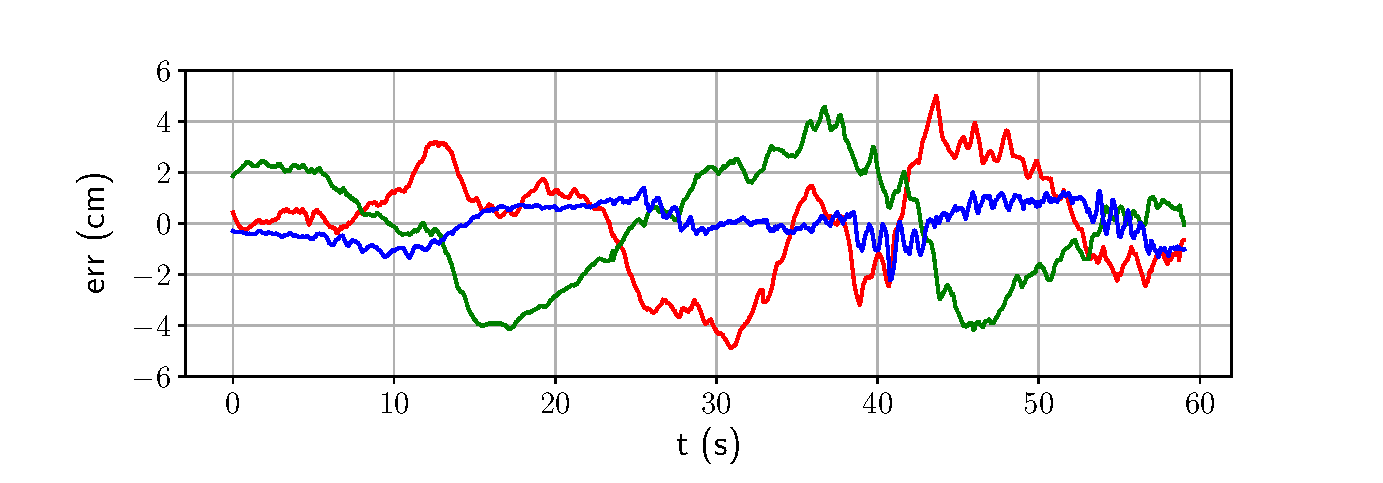
\includegraphics[width=\textwidth]{figures/absolute/terr_loop_twice.eps}
     \end{subfigure}%
     \hfill
     \begin{subfigure}{0.5\textwidth}
         \centering
         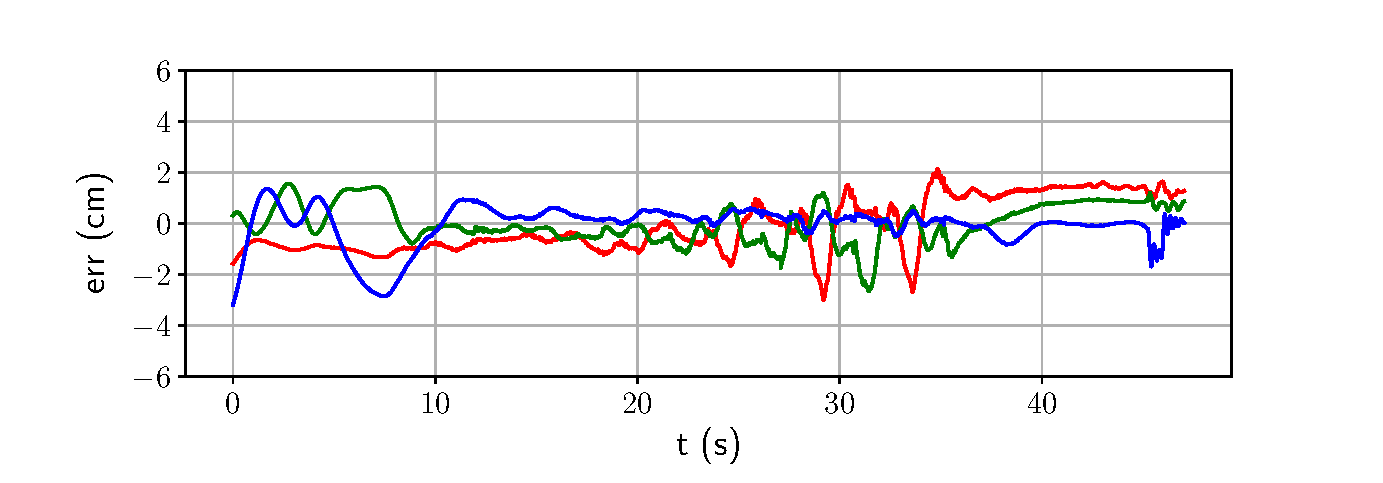
\includegraphics[width=\textwidth]{figures/absolute/terr_stairs1.eps}
     \end{subfigure}%
     \\
    \begin{subfigure}{0.5\textwidth}
         \centering
         \includegraphics[width=\textwidth]{figures/absolute/terr_robot1_walking.eps}
     \end{subfigure}%
     \hfill
     \begin{subfigure}{0.5\textwidth}
         \centering
         \includegraphics[width=\textwidth]{figures/absolute/terr_descending2.eps}
     \end{subfigure}%
    \caption{Translation estimation error (cm) as a function of time (s). In the clock-wise sens, starting from the 
             top-left corner, the datasets are handheld camera, stairs climbing, stairs descending and walking on flat ground. 
             RGB colors correspond to xyz axes.}
    \label{fig:results}
\end{figure}

\subsection{Results}

\subsection{Absolute localization}

We consider four datasets that are summarized in table \tabRef{tab:datasets}. They cover different tasks on which a consistent 
estimation of the robot movement is necessary. The first one is a relatively long sequence consisting of two loops with the VIS handheld. 
This is used to test the long-term localization of the robot, which is interesting for navigation. Secondly, we made the LAAS Gepetto team 
\HRP{2} walk and turn around on a short distance to evaluate the resilience of the filter to the vibrations of the robot. Finally, two more 
challenging datasets are recorded while the robot is climbing and descending stairs. Especially on the latter, the locomotion causes impacts 
that on one hand bring the IMU close to its dynamic range saturation, and on the other hand, provoke images with motion blur. Note that during these experiments, 
the estimator was not used for feedback control. To compare our results with the ground-truth, we used methods described in \cite{zhang2018tutorial} to align 
trajectories given that 4 DoFs are unobservable in VI estimation.
For each case, \keyframes\ are created at a frequency of 6.6 Hz (every 5 images) if tags are detected in the corresponding image.


\figRef{fig:results} presents a quantitative evaluation of the translational errors. In all cases, our estimator achieves errors consistently below a few centimeters. 
The biggest errors are obtained for the walking datasets where the two humps correspond to phases where the robot is turning on itself and sees landmarks that will not be 
seen again later in the trajectory.

\subsection{High-rate velocity estimation}

A high rate estimation of a humanoid robot velocity and in particular of its center of mass is critical for balance controllers. It can be recovered 
from motion capture through numerical differentiation of the positions, but this results in a quite noisy time series. It is especially visible when hard impacts 
make the robot when descending stairs for instance.

\figRef{fig:vz_descending_onestep} presents a zoom-in one part of the stairs descending trajectory. Here, within 2.5 seconds, \HRP{2} lowers 
its base and then its foot touches the next step. The velocity is thus first negative until the impact of the foot on the step. Then, the estimated velocity follows 
a familiar oscillatory damped system behavior while the mocap estimation is more erratic. 

The high rate estimate of the velocity is obtained by integrating IMU measurements with optimally estimated biases from the last \keyframe 
optimized by the solver, as explained in \secRef{sec:publish-state}. The smoothness of the trajectory is a good indicator that the problem has converged to a consistent state.


\begin{figure}[h]
    \centering
    % 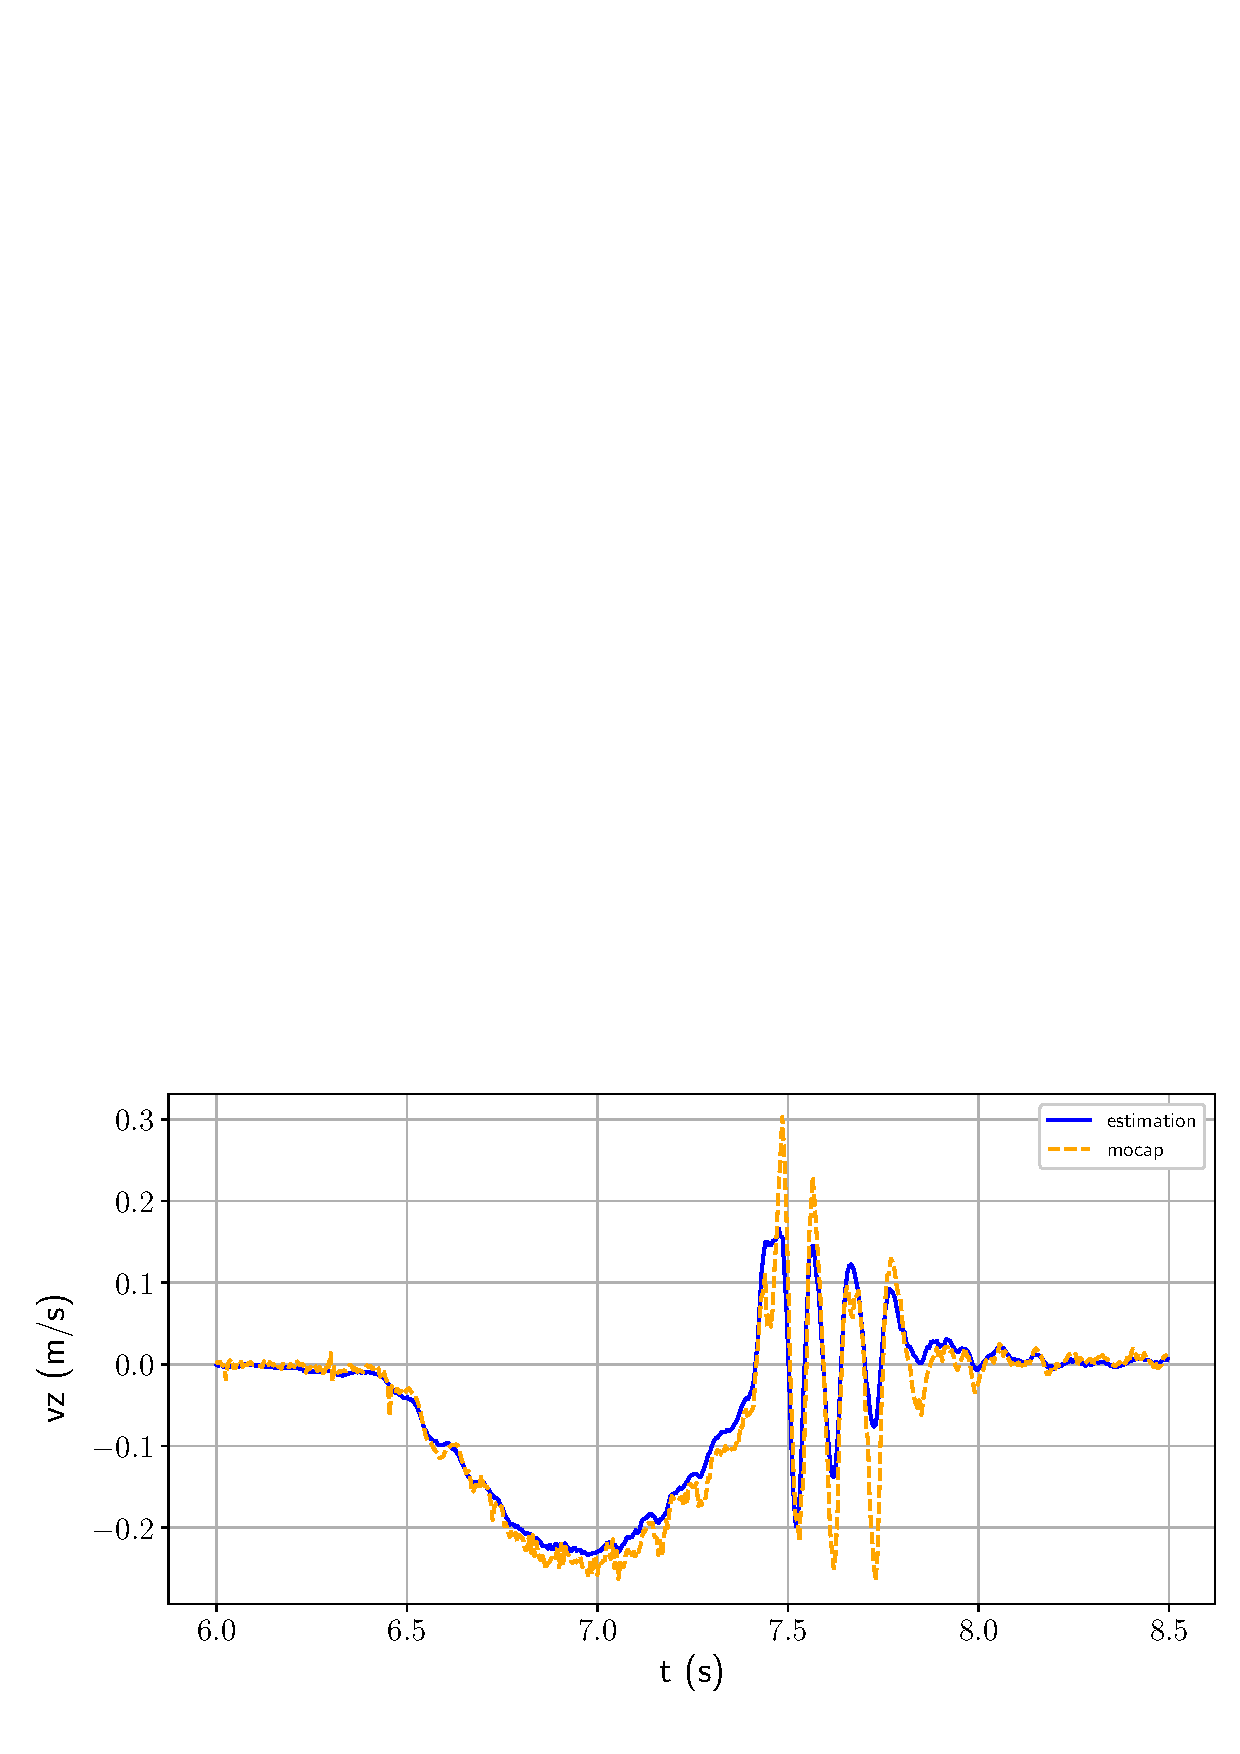
\includegraphics[width=0.8\textwidth]{figures/absolute/vz_descending_onestep.pdf}
    \includegraphics[width=0.9\textwidth]{figures/absolute/vz_descending_onestep_with_kf.pdf}
    \caption{Descending stairs (one step): the robot first lowers its base and then touches the next step with results in vibrations from the impact.
    Vibrations at approximately 10Hz visible in both the motion capture ground-truth and optimal state estimation. Note that the estimation in this case has a smoother curve.
    \keyframes\ are introduced at 6.6Hz (every $\approx 150 ms$) and are represented by vertical red bars. State in between is obtained by applying the pre-integrated 
    delta from the last \keyframe\ to the current time to the estimate of the last \keyframe\ state estimate (see \secRef{sec:publish-state}).}
    \label{fig:vz_descending_onestep}
\end{figure}




\section{Conclusion}

This chapter reports our first experimental results, validating our IMU observation model (using pre-integration), that we assembled into an observable 
estimator using fiducial markers. The implementation reproduces what now is a classical formulation of visual-inertial odometry, but, at the time it was 
released, not demonstrated on a humanoid robot. We have been able to obtain an accurate estimation of the humanoid robot \HRP{2} in a 3D terrain. In particular, 
the IMU enables the estimator to have an excellent accuracy, and high bandwidth in the resulting estimation. In particular, the impact of the feet on the stairs, 
and ensuing vibrations, clearly appears as relevant movement in the estimator output. On the other hand, the fiducial markers enable the filter to display 
a global localization, in particular closing the loop when previously-seen markers where observed again while the 
robot was walking along a loop in the experimental room. This experimentally validates the relevance of fusing these two 
information for localizing a legged robot. In particular, the filter provides a full consistency, on the opposite to loosely-coupled 
filters where the global localization (SLAM-like) is not guaranteed to be consistent with the local estimation of the base state. 

Since this work, a few interesting MAP-based estimators have been deployed on legged robot, as we are going to discuss in the next chapters. 
For the implementation we reported here, we mostly missed some visual odometry (\ie low level geometrical visual features) that would have help the estimator 
to have a better mid-frequency accuracy (between the high-frequency provided by the IMU and the low-frequency provided by the sparse fiducial tracker).
The experimental results were running in real-time by using a fixed window of \keyframes\ active in the estimator and removing the older ones. This
approach may be improved by introducing a marginalization procedure as done in some classical visual-inertial systems \cite{leutenegger2015keyframe}.

In this chapter, we have not yet added the information coming from the foot contact. Moreover, the fiducial markers are not strongly related with any 
relevant part of the robot environment, which makes it difficult to use the localization information into a contact planner. In the next chapters, we are going to show 
how this estimator extends to fully account for the contact information, and directly estimates environment parts that a motion planner could directly used by replacing
the visual front-end.
\chapter{Centroidal estimation}
\label{chp:centroidal_estimation}
\minitoc
\bigskip


In this chapter, we propose a tightly coupled base and centroidal estimator that fuses IMU, kinematics, centroidal kinematics, and force-torque measurements.
This work was first presented in our published paper \cite{fourmy2021contact}.

\section{Introduction}

As mentioned in the literature review, centroidal states are key to the control of legged robots. Indeed, they provide rich information about the general
behavior of the system and can be used to check for the stability of the system. The centroidal state estimation literature is rich, especially for humanoid
robots (see \secRef{sec:centroidal_est_lit}). To our knowledge, all of the centroidal estimators proposed in the literature can be classified as loosely-coupled estimators 
(following the terminology introduced in \secRef{sec:proprio_filters}): they rely on prior knowledge of a base state. For instance, Piperakis \cite{piperakis2018nonlinear} 
describes the whole pipeline: first, an inertial-kinematics EKF estimates the base state, then an EKF uses this fixed base state to obtain centroidal states. 
Since the factor graph optimization framework that we use theoretically reaches its full potential when the maximum number of cross-correlation
are considered, we did not find this solution satisfactory. In \cite{fourmy2021contact}, we proposed a tightly-coupled estimator that jointly estimates
base and centroidal states using IMU, kinematics, and force measurements.


We present results of the application of the estimator on a dataset taken at LAAS-CNRS on the open source robot Solo-12 \cite{grimminger2020open}:
\textit{sinXYZ} corresponds to a trajectory where the robot moves by following a sine wave reference with the feet fixed in place. 
This movement and another one are displayed in the companion video \url{https://peertube.laas.fr/videos/watch/16822d27-3557-4e35-9a0d-ce5b0aea4c27}.

We use the state estimation framework WOLF, developed at IRI-Barcelona, which relies on Google Ceres \cite{ceres-solver} as the graph solver. 
The robot kinematics and dynamics computations are handled by the Pinocchio library \cite{carpentier2019pinocchio}. For all runs, \keyframes\ were created 
at 4Hz for fair comparison.



\section{Problem statement}

We wish need to define an estimator capable to observe both base states (position, orientation, velocity) and centroidal states (CoM, CoM velocity, angular momentum) from proprioception
only. We assume that the following measurements are available on the robot: IMU data, kinematics (leg odometry), centroidal kinematics, and force-torque sensors. 
Since the IMU measurements \eqRef{eq:imu_meas_model} and CoM local position from the kinematics \eqref{eq:com_kine_meas} are biased, we also need to integrate them to the estimated
variables.

Bloesch \cite{bloesch2013state} showed that the base states of legged robots and IMU biases are observable using a tightly coupled estimator based on IMU and kinematics measurements.
On the other end, Rotella \cite{rotella2015humanoid} showed that the centroidal state of a robot and a bias on the centroidal kinematics can be obtained by fusing 
force-torque sensor measurements with centroidal kinematics, based on prior knowledge of the base states. We join the two problems into a single state estimation problem, 
represented by the factor graph of \figRef{fig:centroidal_factor_graph}.  

\begin{figure}[h]
    \centering
    \includegraphics[width=0.6\textwidth]{figures/centroidal/centroidal_factor_graph.pdf}
    \caption{Factor graph representation of the tightly-coupled base-centroidal state estimation problem.
             Each round node corresponds to an estimated state variable with transparent names. Each square corresponds to a factor, that is a measurement residual.
             The color of the residuals are as follow. \textbf{Red}: leg odometry (\secRef{sec:leg_odometry}), \textbf{green}: IMU pre-integration and IMU bias drift 
             (\secRef{sec:preint_residual}, \textbf{purple}: centroidal kinematics (\ref{sec:centroidal_kinematics}, \textbf{blue}: force-torque pre-integration and
             centroidal kinematics bias drift))
             }
    \label{fig:centroidal_factor_graph}
\end{figure}

In this estimator, we have two motion sensors, IMU and force-torque, whose measurements we pre-integrate as explained in \secRef{sec:imu_preint_composite} and
\secRef{sec:force_torque_preint} respectively. Base states and centroidal states are tightly constrained by the centroidal kinematics factor, which relates almost all 
estimation variables at a given \keyframes.

This estimator is implemented in WOLF \cite{sola2021wolf} and is experimentally validated on the Solo-12 quadruped robot as explained in the following sections. 

\section{Experimental setup}
%  
As is often the case with quadruped robots, Solo-12 is not equipped with three axis force sensors at its feet. 
Yet, in order to validate the present method, it is possible to reconstruct the contact forces based on the robot dynamics 
equation \eqref{eq:wbdyn}. Knowing the robot configuration and derivatives $\q,\vq,\dvq$ and joint torques $\bm\tau$ (from motor currents), 
recovering forces from this equation results in solving an over-determined linear system. Some of these quantities are hard to obtain directly 
since they depend on the state being estimated (\eg base orientation) or on numerical differentiation ($\ddqa$). For these reasons, we pre-calculated 
these forces by benefiting from an internal filter of the 3DM-CX5-25 IMU for the base orientation, centered window differentiation of encoder speed 
measurements for the articulation acceleration $\ddqa$ and neglecting the influence of linear velocity. Fig. \figRef{fig:force_est} shows an example of 
the force reconstruction of one leg using the robot proprioceptive sensors.
%
\begin{figure}
    \centering
    \includegraphics[width=0.9\columnwidth]{figures/centroidal/forces_solo_1leg.pdf}
    \caption{Force estimation on X-Y-Z axis (r-g-b) of one Solo-12 leg expressed in world frame using proprioceptive sensors during the \textit{sinXYZ} trajectory}
    \label{fig:force_est}
\end{figure}

\subsection{Base estimation through inertial kinematic fusion}
First, to validate the use of our kinematic factor, we include uniquely the IMU and LO factors to obtain an Inertial Kinematics  estimator which 
conceptually includes the same information as estimators such as \cite{bloesch2013state}. In \figRef{fig:PosiIK4}, we compare our state estimation 
at 1kHz with motion capture (Mo-Cap) up-sampled from 200Hz to 1kHz.
Velocity in base frame is also shown in \figRef{fig:VelIK4}.

\begin{figure}[h]
    \centering
    \includegraphics[width=0.6\textwidth]{figures/centroidal/base_position_IK4.pdf}
    \caption{\textit{sinXYZ} trajectory base position from the IMU+Kinematics (IK) estimator (blue) vs Mo-Cap (red)}
    \label{fig:PosiIK4}
\end{figure}

\begin{figure}[h]
    \centering
    \includegraphics[width=0.6\textwidth]{figures/centroidal/base_velocity_base_frame_IK4.pdf}
    \caption{\textit{sinXYZ} trajectory base velocity in base frame from the IMU+kinematics estimator (blue) vs Mo-Cap (red)}
    \label{fig:VelIK4}
\end{figure}

Artificially removing contact factors (considering only 1, 2 or 3 feet in contact) can help us gain confidence in the use of this kinematic factor 
in situations where we rarely have all feet in contact, like for example with trotting gaits. In \figRef{fig:ErrIKn}, we can see that only considering 
1 foot in contact during the whole trajectory results in a drifting position, but as soon as 2 or more feet are in contact, the system is constrained enough 
for the drift to remain below around 5mm on all axes. 
%
\begin{figure}[h]
    \centering
    \includegraphics[width=0.6\textwidth]{figures/centroidal/base_position_err_IKn.pdf}
    \caption{\textit{sinXYZ} trajectory base position error with different numbers of feet used for the leg odometry factors: 
    1 (blue), 2 (orange), 3 (green), 4 (red) from the IMU+kinematics estimator}
    \label{fig:ErrIKn}
\end{figure}
%

\subsection{Centroidal estimation}

Now, on the same trajectory, we deploy the full estimator with all factors described in Section \figRef{figsec:factor-graph} to jointly 
estimate the base and centroidal quantities. A ground-truth on the centroidal quantities is difficult to obtain since no direct 
sensor can provide us with this information contrary to the base state. 
We can however validate our method by comparing it to a two step procedure: first, estimate the base state with a state Kalman filter as 
implemented in \cite{bledt2018cheetah}, then compute the centroidal quantities directly from the robot kinematic model. 
The full estimator should be able to infer a bias on the $\posim{B}{C}$ measure so we artificially add a constant disturbance 
in the robot dynamic model on the lever of the base link of [0.03, 0.06, 0.04]\,cm, which then corresponds to a CoM bias of 
[-0.0197, -0.0394,  0.0263] cm. \figRef{fig:bias_est} shows that the bias estimated with our method closely matches the introduced bias. 
\figRef{fig:comparison_KF_wolf} shows a comparison between the base and CoM reconstruction with our method and with the two-step base Kalman filter 
with geometric CoM. Note that the base-CoM difference on the z axis reflects the fact that limbs of the robot naturally lowers  its CoM. 
The estimated CoM velocity closely follows the velocity of the base as shown in \figRef{fig:com_base_vel}.


\begin{figure}[h]
    \centering
    \includegraphics[width=0.6\textwidth]{figures/centroidal/com_position_povcdl_sin.pdf}
    \caption{Base position (blue) vs CoM (red) from the full estimator}
    \label{default}
\end{figure}

\begin{figure}[h]
    \centering
    \includegraphics[width=0.6\textwidth]{figures/centroidal/com_velocity_povcdl_sin.pdf}
    \caption{Base (blue) vs CoM (red) velocities   from the full estimator}
    \label{fig:com_base_vel}
\end{figure}


\begin{figure}[h]
    \centering
    \includegraphics[width=0.6\textwidth]{figures/centroidal/com_bias_est.pdf}
    \caption{Estimation of bias on CoM measurement from the full estimator along x-y-z axis ( red-green-blue) in base frame}
    \label{fig:bias_est}
\end{figure}

\begin{figure}[t]
    \centering
    \includegraphics[width=0.6\textwidth]{figures/centroidal/base_com_position_wolf_vs_KF.pdf}
    \caption{Comparison of the estimates between decoupled the Kalman filter base estimator and geometric CoM reconstruction (blue) and 
    the tightly coupled estimator presented in this paper (red) on the \textit{sinXYZ} trajectory with artificial base link CoM bias.}
    \label{fig:comparison_KF_wolf}
\end{figure}



\chapter{Cosy SLAM}
\label{chp:cosyslam}
\minitoc
\bigskip


In this chapter we present a visual-inertial SLAM system based on a deep-learning-based pose estimation libary \cite{labbe2020cosypose}.
We present experimental results from our paper \cite{debeunne2021cosyslam} (submitted at ICRA22).

\section{Introduction}
Navigation of legged robots using onboard exteroceptive sensors has gained a lot of traction in recent years due to their progressive deployment for 
industrial applications \cite{bellicoso2018advances}. 
For repeated travels, the map-less teach and repeat methods \cite{furgale2010visual, mattamala2021learning} avoid the need of a metric and globally coherent localization 
by benefiting from the knowledge of a human operator. This works very well for applications in which such supervision is available, and a global map is not. 
% However, many times, in industrial environments, a map is obtainable as a CAD model or 3D scans, in which important assets can be labeled.
Building a metric and semantic map of the environment may be useful to automatize navigation and exploration in larger environments. Besides,
standard objects whose CAD model is known (such as gauges, valves, stairs, etc.) may often appear.

Many representations of the environment are possible depending on the needs of the system. In \cite{fallon2014drift} a prior map defined as a LIDAR point-cloud is 
used in a Gaussian particle filter to localize a humanoid robot and perform online foot planning. Fankhauser \cite{fankhauser2014robot} takes as an input 
an external odometry source to produce efficient robot-centric elevation maps while \cite{kim2020vision} builds a global height map to navigate through cluttered 
environments. Other approaches \cite{wisth2021vilens} rely on a tight fusion between proprioceptive and exteroceptive sensors to make the odometry more robust. 
A full overview of these systems can be found in our literature review (\secRef{sec:environment_awareness}).

\begin{figure}[h]
  \centering
  \includegraphics[width=0.80\textwidth]{figures/cosyslam/solo_closer_small.png}
  \caption{Experimental setup: a Realsense D435i is mounted on the Solo robot that localizes itself \wrt stairs. A motion capture system provides ground 
            truth of the robot pose.}
  \label{fig:solo_and_stairs}
\end{figure}

These approaches build metric maps that do not usually leverage the presence of known assets in the scene, although a few examples in the computer vision literature 
exist. In \cite{SalasMoreno2013SLAMSL}, the authors develop one of the first object-level SLAM algorithms from a depth sensor. Using a voting process based on point-cloud descriptors, 
a simultaneous recognition and pose estimation of known objects was performed and included as factors in a graph optimization estimator. 
The method benefited from an active search of the objects in the scene, the detection being done in the SLAM loop.
Aside from the robot trajectory and poses of objects, \cite{sucar2020nodeslam} also proposes to optimize the object shapes using a differentiable 
rendering engine. In such approaches, objects need to be detected, classified, and their relative pose \wrt the camera has to be integrated into the estimator. 
On the other end, a work like \cite{pillai2015monocular} uses a semi-dense mono camera SLAM algorithm to produce a scale-ambiguous feature map. 
Then, a descriptor-based multi-view object proposal is performed as a post-processing step. 



% Huge progress to the field of object detection was brought about by the advent of CNN frameworks such as \cite{he2018mask}. As a result, it seems that the domain of 
% object scene reconstruction is now dominated by methods relying only on RGB cameras, for both object detection and pose retrieval. A major example is the framework CosyPose 
% \cite{labbe2020cosypose}. This approach mixes a new state-of-the-art single-view pose estimation algorithm with a multi-view algorithm using RANSAC and Bundle Adjustment. 
% It achieved first in most of the 2020 BOP challenge categories \cite{hodavn2020bop}. This system obtains precision in the order of centimeters on real objects whose 3D 
% model is known. 
% Its performances make it a good candidate as a direct 6D pose sensor to perform multi-sensor fusion. In the context of legged robots, this is very useful to localize the 
% robot \wrt objects it needs to interact with, such as objects to manipulate or stairs to climb. 
% %However, due to a current lack of generalization capability, the trained models cannot be directly used for objects that are not part of its training.
% While these models are not yet able to be generalized to classes of objects, rapid progress is expected in this direction. Their performances are already very interesting 
% to help with the locomotion in known scenes.

%Another thing that is not handled by CosyPose was the assessment of the uncertainty of measurements from the different objects in the scene, which depends on a variety 
% of parameters such as object occlusion and distance. 
% When considering merging a tracker such as CosyPose with other sensor modalities, an important aspect is to predict covariance representing the level of confidence in 
% the tracker estimate.
% Such data uncertainty awareness has been shown to be crucial to the robustness of SLAM systems involving neural networks subsystems such as \cite{yang2020d3vo}, 
% while \cite{SalasMoreno2013SLAMSL} claimed to compute a covariance matrix approximated as the inverse of the Iterative Closest Point output. The methods targeted for 
% deep learning applications are harder to implement, especially if the goal is to use an off-the-shelf pose estimation neural network, as it is the case for this paper. 
% For instance, Bayesian Neural Networks \cite{jospin2020hands} need to be trained explicitly for uncertainty prediction while Monte Carlo (MC) Dropout \cite{gal2016dropout} 
% requires multiple forward passes at run-time.


As described in \secRef{sec:object_pose_est_algos}, deep-learning-based object detection systems have now reached an accuracy that make them candidates for mobile robotics applications.
Applications range from robot manipulation, like sorting known objects, or localization \wrt known assets. For this last application, however,
the direct output of CosyPose is not sufficient for two reasons. First, many objects have strong symmetries, which makes CosyPose orientation estimation jumps from one to the other
depending on the frames. This output has, therefore, to be filtered using prior knowledge about the world or the robot's movements. Second, the robot needs to keep
a memory of objects it has seen when they go out of its field of view.

To address the challenges, we presented in \cite{debeunne2021cosyslam} a practical implementation of a SLAM system based on the design of an off-the-shelf 
deep-learning object pose estimation algorithm \cite{labbe2020cosypose}. To integrate CosyPose measurements with other sensors, we propose a noise model based 
on empirical data, presented in \secRef{sec:cosypose_covariance}. We also detail implementation details to circumvent outliers in the network output. 
Experimental validations were conducted with a visual-inertial system, both handheld and mounted on a quadruped robot. Finally, we fine-tuned the pre-trained models 
to perform stairs localization, as explained in \secRef{sec:retraining_with_stairs}. 




\section{Implementation of the Visual Inertial filter}

\subsection{Factor Graph formulation}
This section will be very short so as not to repeat ourselves: the problem has the same structure as the \apriltag-IMU VI system presented in \chpRef{chp:absolute_vi}, 
thus it as the same factor graph \figRef{fig:VI_factor_graph}. The \apriltag\ pose measurement model is replaced by the CosyPose measurement model, presented in \secRef{sec:learning_based_object_pose_est}.


\subsection{Data association and Outlier rejection}
A key part of our SLAM system is the association of landmarks with the rejection of erroneous pose estimates. First of all, each object is associated with a 
label $\alpha$ so that a detection can only match a landmark with the same label. Then, the position of the robot is propagated by integrating the IMU measurements 
with the current biases estimates. Thus, each detected object pose can be transformed in the world frame using the propagated robot state. We check if this pose is 
similar to the one of a landmark with the same label with a threshold on the distance between the poses in $SE(3)$. 
If a detection does not match any landmark then a new landmark is created.

CosyPose can return poses of objects that are not included in the scene because of false detections, of Mask-RCNN, or wrong pose estimations (most often due to object symmetries). 
To handle these outlier detections, each landmark is associated with a score $c$ that corresponds to its repeatability over time: 

\begin{equation}
    c = \frac{n_f}{\Delta t}
\end{equation}

$\Delta t$ is the time since the landmark initialization and $n_f$ is the number of factors associated with it.
The lowest scores are filtered with a threshold determined empirically and the associated landmarks are removed from the map.




\section{Experimental validation}

We have produced datasets in the robotic experimental arena at LAAS-CNRS in Toulouse. This is a 3D environment about $10 m \times 5m$ made of flat floors, 
stairs and beams. The robot environment was augmented with objects of the datasets that were used to train CosyPose. Each dataset is composed of three data sources:

\begin{itemize}
    \item A sequence of RGB images (30 Hz)
    \item A sequence of IMU measurements (200 Hz)
    \item A sequence of motion capture (MoCap) measurements (200 Hz), used as ground-truth 
\end{itemize}

We recorded two types of datasets: one for the uncertainty models and one for SLAM experiments. For the uncertainty models, reflective MoCap markers 
were attached to the object to obtain the ground-truth of their pose. For the SLAM, only the camera was tracked. We used the monocular RGB camera and the Bosh BMI085 
IMU of an Intel Realsense L515 Camera for handheld trajectories. The Intel Realsense d435i was used with the same modalities 
for the experiments on the quadruped robot Solo \cite{grimminger2020open} as shown in \figRef{fig:solo_and_stairs}. 
The extrinsic calibration between the IMU and the camera was provided by Intel and the delays observed between IMU and Camera measurements were negligible. 
Our datasets are publicly available at \url{https://homepages.laas.fr/mfourmy/icra22_cosyslam}.





\subsection{Object level VI-SLAM}

\begin{figure}[h]
  \centering
  \includegraphics[width=0.9\textwidth]{figures/cosyslam/trajectory_circular.png}
  \caption{Comparison between the MoCap, the output of CosySLAM with visual factors only and the output of CosySLAM with IMU fusion on the circular trajectory.}
  \label{fig:traj_circular}
\end{figure}

In order to validate the performances of the fusion of CosyPose estimates and inertial measurements, we evaluated three scenarios with the camera held by hand and 
T-LESS objects\footnote{T-LESS is one of the dataset for which CosyPose is trained by default and whose object can be bought in Czech Republic~\cite{hodan17t}. 
It features several small electric devices, whose symmetry at lack of texture make them an interesting benchmark for realistic scenarios.} in the scene. 
The first one is a short and slow trajectory, \ie an ideal scenario. The second one is a slow but long trajectory, to validate the consistency of our system over time. 
The last one is a highly dynamic scenario with a lot of motion that can blur some frames and lose sight of objects for more extended periods. 
Moreover, T-LESS objects being the most difficult objects for pose estimation with CosyPose, they may return many outliers and noisy measurements. 
This is therefore a challenging dataset to test the robustness of our algorithm. \Keyframes\ are selected at 10 Hz, only if objects are detected in the images.

\begin{table}[h]
    \begin{center}
    \caption{Datasets description and results of the hand held videos}
    \label{tab:tless}
    % \begin{tabular}{|c|c{1.1cm}|c{1.1cm}|c{1.1cm}|c{1cm}|}
    \begin{tabular}{|c|c|c|c|c|}
        \hline 
        Scenario  & Length(m) & Duration(s) & MTE¹(cm) & STE²(cm) \\
        \hline 
         V-only - Circular & 3.7 & 23.7 & 3.8 & 1.6\\
        \hline 
         V-only - Short & 2.5 & 12 & 3.8 & 2.4 \\
        \hline 
         V-only - Dynamic & 3.5 & 17.8 & 7.8 & 4.0  \\
        \hline 
         V-IMU - Circular & 3.7 & 23.7 & 1.9 & 0.7\\
        \hline 
         V-IMU - Short & 2.5 & 12 & 1.9 & 0.5 \\
        \hline 
         V-IMU - Dynamic & 3.5 & 17.8 & 1.7 & 1.2  \\
        \hline
    \end{tabular}
    \end{center}
¹ Mean translation error \\
² Standard deviation of translation error
\end{table}

It is interesting to analyze the gains brought by the IMU fusion. The most evident observation is that the output trajectory is smoother, which gives more consistency 
to the result (\figRef{fig:traj_circular}). But we can notice that the MTE is also reduced (\tabRef{tab:tless}). Indeed, the motion model is more precise thanks 
to IMU data. This makes the outlier rejection more efficient than the visual-only CosySLAM which makes a zero velocity assumption between \keyframes.




\subsection{Localization and Mapping of stairs by Solo}

With our retrained model (\secRef{sec:retraining_with_stairs}) we were able to perform SLAM in our experimental area, without augmenting it with other objects. 
We recorded video sequences including stairs with a camera fixed on a Solo robot (\figRef{fig:map_stairs}). A stair has three discrete symmetries 
that are hard to handle for an object pose estimator and the images provided by Solo were noisy because of the walk. 
These scenarios are challenging for our SLAM system, but it maps successfully the stairs and the error on the position of the base of Solo remains reasonable 
(\tabRef{tab:solo}).

\begin{table}[h]
   \begin{center}
   \caption{Datasets description and results of the videos taken on Solo}
   \label{tab:solo}
    % \begin{tabular}{|c{2.2c1cm}|c{1.1cm}|c{1cm}|c{1cm}|}
    \begin{tabular}{|c|c|c|c|c|}
        \hline 
        Scenario  & Length(m) & Duration(s) & MTE(cm) & STE(cm) \\
        \hline 
         V-IMU - Approach & 1.3 & 18.7 & 2.0 & 0.9\\
        \hline 
         V-IMU - Module & 1.3 & 15.5 & 2.4 & 1.5 \\
        \hline
    \end{tabular}
    \end{center}
\end{table}

\begin{figure}[!ht]
  \centering
  \includegraphics[width=\linewidth]{figures/cosyslam/mapped_stairs.png}
  \caption{This trajectory was recorded on Solo walking along a climbing module made of three stairs using a walking controller \cite{leziart2021implementation}. 
  The green dots represent the trajectory of Solo provided by the MoCap, and the red dots the one produced by our visual-inertial SLAM. 
  The blue rectangles represent the map of the SLAM made of stairs.}
  \label{fig:map_stairs}
\end{figure}

\chapter{A new proprioceptive and vision dataset}

This short chapter presents a dataset that we recently produced with Gepetto team's quadruped robot Solo-12. This dataset was acquired in our experimental space 
in LAAS-CNRS (see \figRef{fig:solo_dataset_scene}) and includes several walking trajectories using the controller \cite{leziart2021implementation}. We remote-controlled the robot in a scene augmented 
with \apriltags\ and elements from the T-less dataset, recording proprioceptive and exteroceptive measurements. 

\begin{figure}[h]
    \centering
    \includegraphics[width=0.95\textwidth]{figures/solo_dataset_scene.png}
    \caption{Solo quadruped in the experimental room.}
    \label{fig:solo_dataset_scene}
\end{figure}

The recorded sensor measurements include joint encoders, joint current, IMU from Solo onboard sensing as well as a RealSense D435i RGB camera and IMU.
Controller logs (such as the planned feet contacts timings) are also recorded. The RealSense was fixed at the front of the robot, slightly down-facing (30 degrees).
A summary of available data is reported in \tabRef{tab:dataset_solo}. Calibration data using a fiducial marker grid obtained before the experiments to 
calibrate the image distortion, camera-IMU relative transformation, and potential time-shift of the RealSense system. A sample image of one of the trajectories
is shown in \figRef{fig:solo_dataset_image}.
External video recordings of each experiment were taken.

\begin{table}[h]
    \centering
    \caption{Summary of available data sources from Solo-12 onboard sensing and RealSense D435i}
    \begin{tabular}{|llll|}
        \hline
        \thead[l]{Type} & \thead[l]{Source} & \thead[l]{Details} & \thead[l]{Frequency}  \\
        \hline
        Joint currents & Solo-12 &  & 1kHz  \\
        \hline
        IMU            & Solo-12 & \makecell[l]{3DM-CX5-25 \\ LORD Microstrain} & 1kHz  \\
        \hline
        RGB images & Solo-12 & \makecell[l]{1920 × 1080 \\ rolling shutter} & 30Hz  \\
        \hline
        IMU            & RealSense & Bosch BMI055 & 200Hz  \\
        \hline
        Ground truth & Qualysis Motion Capture &  & 200Hz \\
        \hline
    \end{tabular}
    \label{tab:dataset_solo}
\end{table}


All data from Solo's onboard sensing is hardware synchronized. Similarly, the RealSense IMU and RGB images streams are synchronized. However, 
we do not have the possibility to hardware synchronize the RealSense with Solo yet. Instead, we plan to rely on the correlation between Solo's IMU and the RealSense IMU
to synchronize the streams of data in a post-processing step. To this end, we proceeded to a synchronization procedure at the beginning of each trajectory by
tapping on the robot a few times. This precise signal should be enough to align both IMU time series and, thus, the rest of the sensor streams.


Recorded trajectories (2 minutes each) include motions of increasing difficulty, with forward-backward walking in a straight line, a square path around the scene, and
loopy trajectories. With this dataset, we plan to implement an estimator fusing inertial, kinematics, and object-level transformation based on our previous work.
This dataset will serve to benchmark an integration work destined to obtain an estimator for both balance control states (orientation, velocity) and 
global localization through object-level SLAM. The loopy trajectories in particular will serve to display the behavior of the estimator when closing longer loops.


\begin{figure}[h]
    \centering
    \includegraphics[width=0.7\textwidth]{figures/solo_dataset_image.png}
    \caption{Example of an image captured with the RealSense attached to Solo while walking.}
    \label{fig:solo_dataset_image}
\end{figure}
% \part{Conlusion}
Just the conclusion

% \appendix

\chapter{Pre-integration details}
\section{Justification of \cite{forster2017-TRO} delta formulas}
We detail here how the delta formulas of equation \eqRef{eq:IMUPreintim} can be derived from \eqRef{eq:IMUIntim}.

The rotation one is easy to get, multiplying by $\Rot{}{}^{i,T}$:
\begin{equation}
    \DR_{im} \triangleq \Rot{}{}^{i,T} \Rot{}{}^{m} = \prod_{k=i}^{m} \Exp((\angvelm{}{}^k - \bias_{\angvel{}{}}^k - \noise_{\angvel{}{}}^k)\dt)
    \label{eq:IMUDeltaR}
\end{equation}

The velocity is as well quite easy, by defining $\Dt_{im} \triangleq \sum_{k=i}^{m} \dt = (m-i)\dt$:
\begin{equation}
    \Dv_{im} \triangleq \Rot{}{}^{i,T} (\vel{}{m} - \vel{}{i} - g \Dt_{im}) 
    = \prod_{k=i}^{m} \DR_{ik} \Exp((\accm{}{}^k - \bias_{\acc{}{}}^k - \noise_{\acc{}{}}^k)\dt)
    \label{eq:IMUDeltav}
\end{equation}

The position delta requires more calculations. First, inject equation \eqRef{eq:IMUDeltav} in the position equation of \eqRef{eq:IMUIntim} then rearrange and reorder the terms.

\begin{equation}
\begin{split}
\posi{}{}^{m} - \posi{}{}^{i} &= \sum_{k=i}^{m} \Big[
(\vel{}{}^i + \grav \Dt_{ik} + \Rot{}{}^i \Dv_{ik})\dt 
+ \frac{1}{2}\grav \dt^2 + \frac{1}{2}\Rot{}{}^{k}(\accm{}{}^k - \bias_{\acc{}{}}^k - \noise_{\acc{}{}}^k)\dt^2 \Big]
\\
&= \vel{}{}^i \Dt_{im} + 
\grav\sum_{k=i}^{m} \Dt_{ik} \dt + \frac{1}{2}\grav \sum_{k=i}^{m} \dt^2 +
\Rot{}{}^i\sum_{k=i}^{m} \Big[\Dv_{ik}\dt +  \frac{1}{2} \DR_{ik} (\accm{}{}^k - \bias_{\acc{}{}}^k - \noise_{\acc{}{}}^k)\dt^2 \Big]
\\
&= \vel{}{}^i \Dt_{im} + 
\grav \sum_{k=i}^{m} (\Dt_{ik} \dt + \frac{1}{2}\dt^2) +
\Rot{}{}^i\sum_{k=i}^{m} \Big[\Dv_{ik}\dt +  \frac{1}{2} \DR_{ik} (\accm{}{}^k - \bias_{\acc{}{}}^k - \noise_{\acc{}{}}^k)\dt^2 \Big]
\end{split}
\end{equation}

We will simplify the gravity term that we will call $\mathcal{G}t_{im}$. Noting that:

\begin{equation*}
    \sum_{k=i}^{m}k = \sum_{k=1}^{m}k - \sum_{k=1}^{i-1}k = \frac{m(m-1)}{2} - \frac{i(i-1)}{2} 
\end{equation*}

we can deduce that:

\begin{equation*}
\begin{split}
\mathcal{G}t_{im} 
&= \dt \sum_{k=i}^{m}(\Dt_{ik} + \frac{1}{2}\dt) = \dt \sum_{k=i}^{m}((k -i)\dt + \frac{1}{2}\dt)
\\
&= \dt \Big[ \sum_{k=i}^{m} [ k \dt - i(m-i)\dt ] + \frac{1}{2}\Dt_{im}  \Big] 
\\
&= \dt \Big[ \frac{\dt}{2} (m(m-1) - i(i-1) - 2i(m-1)) + \frac{1}{2}\Dt_{im} \Big] 
\\
&= \dt \Big[ \frac{\dt}{2} (i^2 - 2im + m^2 + i - m) + \frac{1}{2}\Dt_{im} \Big] 
\\
&= \dt \Big[ \frac{1}{2} (m-i)^2dt - \frac{1}{2}(m - i)\dt + \frac{1}{2}\Dt_{im} \Big]
\\
&= \frac{1}{2} (m-i)^2dt^2 = \frac{1}{2} \Dt_{im}^2
\end{split}
\end{equation*}
Multiplying by $\Rot{}{}^{i,T}$ and reordering the terms, we can finally define a position delta quantity:

\begin{equation}
    \Dp_{im} \triangleq \Rot{}{}^{i,T}(\posi{}{}^m - \posi{}{}^i - \vel{}{}^i \Dt_{im} - \frac{1}{2} \grav \Dt_{im}^2) = 
    \sum_{k=i}^{m} \Big[\Dv_{ik}\dt +  \frac{1}{2} \DR_{ik} (\accm{}{}^k - \bias_{\acc{}{}}^k - \noise_{\acc{}{}}^k)\dt^2 \Big]
\end{equation}


\section{Elements of the IMU delta matrix Lie group}


\subsection{Tangent space and Lie algebra \texorpdfstring{$\mathfrak{d}$}{d}}
\cite{sola2018micro}
Following \cite{sola2018micro}, the tangent space of $\cD$ at the point $\D$ is found by taking the time derivative of the group constraint, $\D\inv\D = \bfI$.
Noting $\dot{\bullet} \te \dpar{\bullet}{t}$, this yields 
% the tangent space constraint, $\D\inv\dot\D+\dot{(\D\inv)}\D=0$.
% This gives 
after a few manipulations
%
\begin{align}\label{equ:constr}
\D\inv\dot\D 
&=
\begin{bsmallmatrix}
\hatx{\bw} & ~~\DR\tr\bfa~~ & \DR\tr(\bfv-\Dv) \\
\bf0 & 0 & 1 \\
\bf0 & 0 & 0 
\end{bsmallmatrix}
~,
\end{align}
%
with $\bfv \te \dot\Dp$, $\bfa \te \dot\Dv$ and $\hatx{\bw} \te \DR\tr\dot\DR$.
% The equation above defines the tangent space at the point $\D$. 
The Lie algebra $\mathfrak{d}$ is the tangent space at the identity $\D=\bfI$.
Its elements $\bm\nu\hhat 
\te \dot\D |_{\D=\bfI}$ and their isomorphics $\bm\nu$ in Cartesian space are given by, % $\D=\bfI$, so
%
\begin{align}
\bm\nu\hhat 
% \te \dot\D |_{\D=\bfI}
&=
\begin{bsmallmatrix}
\hatx{\bw} & \bfa & \bfv \\
\bf0 & 0 & 1 \\
\bf0 & 0 & 0 
\end{bsmallmatrix} \in \mathfrak{d}
~~~\xrightleftharpoons[\wedge]{~\vee~}~~~ 
\bm\nu=\begin{bsmallmatrix}
\bfv \\ \bfa \\ \bw \\ 1
\end{bsmallmatrix} \in\bbR^{10}
~.
\end{align}
%
This tangent $\bm\nu\hhat$ corresponds to the `velocity' of the group element. 
Any point in the Lie algebra can be obtained after moving at constant velocity during a period $\Dt$, that is, $\bftau\hhat=\bm\nu\hhat\Dt\in\mathfrak{d}$ ---see \eqRef{equ:lie_algebra}.
%
\subsection{The exponential map}
\subsubsection{The general case}
Eq.~\eqRef{equ:constr} can be written as $\dot\D=\D\cdot\bm\nu\hhat$.
This is an ordinary differential equation whose  integral for constant $\bm\nu$ yields the exponential map \cite{sola2018micro}, $ \D(t) = \exp\left(\bm\nu\hhat t\right)$.
This gives a direct expression of the integral of information of the type $(\bfv,\bfa,\bw)$ onto the deltas manifold. See below for the $(\bfa,\bw)$ case.
The closed form of the exponential map is obtained through Taylor expansion (see \eg\ \cite{sola2018micro}\ for examples). 
At $t=\Dt$ we have,
%
\begin{align}
\D(\Dt) 
&= \exp(\bm\nu\hhat\Dt) \te \sum_n \frac1{n!}(\bm\nu\hhat\Dt)^n
~.
\end{align}
%
% with $\bfA=\bftau\hhat\Dt$.
%
Exploiting the cyclic pattern of the powers of $\hatx{\bw}$, this results in
%
\begin{align}
\exp\left(\begin{bsmallmatrix}
\hatx{\bw} & \bfa & \bfv \\
\bf0 & 0 & 1 \\
\bf0 & 0 & 0 
\end{bsmallmatrix}\Dt\right) 
\!=\! \begin{bsmallmatrix}
\exp(\hatx{\bw}\Dt) & \bfQ\bfa\Dt\, & \bfQ\bfv\Dt+\bfP\bfa\Dt^2 \\
\bf0 & 1 & \Dt \\
\bf0 & 0 & 1
\end{bsmallmatrix}
\end{align}
%
with (we skip proofs for space reasons)
%
\begin{align} \label{equ:RQP}
% \bfR (\bth)
%  &= \exp(\hatx{\bth})
%   = \bfI + \sin\theta\hatx{\bfu} + (1-\cos\theta)\hatx{\bfu}^2\\
\bfQ (\bth)
 &= 
  \bfI + \frac{1-\cos\theta}{\theta}\hatx{\bfu} + \frac{\theta-\sin\theta}{\theta}\hatx{\bfu}^2\\
\bfP (\bth)
 &= 
  \frac12\bfI 
   + \frac{\theta-\sin\theta}{\theta^2}\hatx{\bfu} 
   + \frac{\cos\theta + \frac12\theta^2 - 1}{\theta^2}\hatx{\bfu}^2
~,
\end{align}
%
where  $\bth=\bw\Dt$, $\theta=\norm{\bth}$ and $\bfu=\bth/\theta$ form the angle-axis representation of the rotation step $\bw\Dt$. 


\subsubsection{The IMU case of \texorpdfstring{$\bfv=0$}{bfv=0}}
\label{sec:IMU_case}

We defined the IMU deltas as the motion relative to the free-falling frame, which has initial velocity $\bfv_i$. 
Thus the tangent velocity $\bfv=\dot\Dp$  is zero at the start of the integration step. 
%
Since the exponential $\Exp(\bm\nu\Dt)$ assumes a constant tangent vector $\bm\nu=(\bfv,\bfa,\bw,1)$ during the interval $\Dt$, we have that $\bfv=0$ during the full step. 
%
This gives immediately
%
\begin{align}
% \D &= 
\exp\left(\begin{bsmallmatrix}
\hatx{\bw} & \bfa & \bf0 \\
\bf0 & 0 & 1 \\
\bf0 & 0 & 0 
\end{bsmallmatrix}\Dt\right) 
= \begin{bsmallmatrix}
\exp(\hatx{\bw}\Dt) & ~\bfQ\bfa\Dt~ & \bfP\bfa\Dt^2 \\
\bf0 & 1 & \Dt \\
\bf0 & 0 & 1
\end{bsmallmatrix}
~.
\end{align}




\subsection{The adjoint and small adjoint matrices}

%
Following the general methodology explained in \cite{sola2018micro}, the adjoint matrix is obtained by identifying the linear terms in $\Ad{\D}\bftau=(\D\bftau\hhat\D\inv)\vvee$. We get after long but relatively easy calculations,
%
\begin{align}\label{equ:Ad}
\Ad{\D} &=
\begin{bsmallmatrix}
\DR & -\DR\Dt & \hatx{\Dp-\Dv\Dt}\DR & \Dv \\
\bf0 & \DR & \hatx{\Dv}\DR & \bf0 \\
\bf0 & \bf0 & \DR & \bf0 \\
\bf0 & \bf0 & \bf0 & 1
\end{bsmallmatrix} 
\quad
\in\bbR^{10\times10}~.
\end{align}



Similarly, from \cite{EADE-18-DERIVATIVE} the small adjoint matrix can be computed by identifying the linear terms in $
\ad{\bftau}\bfsigma = 
(\bftau\hhat\bfsigma\hhat-\bfsigma\hhat\bftau\hhat)^\vee
$
%
which  for $\bftau=(\bfrho,\bfupsilon,\bth,\Dt)\in\mathfrak{d}$ yields,
%
\begin{align}\label{equ:ad}
\mathrm{\bf ad}_\bftau = \begin{bsmallmatrix}
\hatx{\bth} & -\bfI\Dt & \hatx{\bfrho} & \bfupsilon \\
\bf0 & \hatx{\bth} & \hatx{\bfupsilon} & \bf0 \\
\bf0 & \bf0 & \hatx{\bth} & \bf0 \\
\bf0 & \bf0 & \bf0 & 0 
\end{bsmallmatrix}
\quad
\in\bbR^{10\times10}~.
\end{align}




\subsection{The right Jacobian}

The right Jacobian $\mjac{}{r}$ is the Jacobian of $\Exp()$ as described in \cite{sola2018micro}.
Lacking at the moment a closed form for it, we take the general methodology for the left Jacobian described in \cite{EADE-18-DERIVATIVE}, and transform it to the right using $\mjac{}{r}(\bftau)=\mjac{}{l}(-\bftau)$ \cite{sola2018micro},
%
\begin{align}\label{equ:Jr}
\mjac{}{r}(\bftau) 
= \mjac{}{l}(-\bftau) 
= \sum_i \frac{\ad{-\bftau}^i}{(i+1)!}
= \sum_i \frac{(-\ad{\bftau})^i}{(i+1)!}
% ~
% \in\bbR^{10\times10}
~.
\end{align}
%
This sum can be truncated at the desired degree of accuracy.






\section{Jacobians of force/torque pre-integration}

TODO



% \listoffigures
% \listoftables

% \newpage

\noindent\makebox[\linewidth]{\rule{0.6\textwidth}{2pt}}

\small

\paragraph{Abstract}~

Legged robots are complex mechanisms whose stable behavior depends on the proper estimation of several different quantities that must be observed at 
high speed and accuracy. While the robot state can mostly not be observed directly by any existing sensors, it is typically reconstructed by fusing very 
diverse sensor modalities.
These sources of information differ significantly on their acquisition frequencies, the nature of the data, and the computational processing cost. 
While state estimation by sensor fusion is a common topic to most robotic platforms, it offers a particular challenge in legged robotics by their peculiar dynamics.
For legged robots, on the one hand, the robot state is needed to maintain its sense of balance and locomote safely, and, on the other hand, a precise representation 
of the environment is required for navigation and interaction. 

The current approach for many legged systems, in the literature, solve
these problems independently, using cascades of estimators that may neglect some of the correlation present in the data.
This artificial decoupling acts as strong priors that enable simple estimators to handle the estimation of each part of the cascade and stabilize 
the behavior of the overall estimation scheme. On the other hand, designing a cascade involves a lot of specialized work that hardly generalizes to new 
scenarios or new sensor modalities.
In this thesis, we rather defend the idea of building a single tightly-coupled estimator capable of estimating all quantities needed by the robot. 
For this goal, the framework of a-posteriori estimation, formalized as a factor graph, is very suitable. This assertion does not come as a surprise, 
as factor graphs are nowadays highly popular in the SLAM literature, yet they are still under-represented in legged robots systems.

In this thesis, we investigate a few avenues that we believe are crucial to achieving these goals. First, we develop tailored sensor measurement models 
with attention to the correct mathematical formulation involving Lie theory.
Second, we propose visual-inertial systems based on object-level detection that provide relative transformation between the camera and the objects.
We provide covariance models for two kinds of objects: the first one is an analytical model for fiducial markers~; the second
is an empirical model for deep-learning-based object pose estimation.
Third, we handle high-rate sensors by developing a generalization of the IMU pre-integration theory. We propose a new formulation of the IMU
pre-integration based on compact Lie groups. 
Fourth, we show that pre-integration can also be applied to use force-torque sensors found on legged robots. 
By fusing it with a leg-kinematics based odometry and IMU, we show that this new formulation makes possible the tightly-coupled estimation
of centroidal quantities within the context of Factor Graph estimation.

The proposed theoretical ideas are implemented in a coherent estimation framework, extending the factor-graph software Wolf. Each new modality is 
validated in a dedicated experimental setup that allowed us to quantify its interest and relevance for legged robotics.



\paragraph{Keywords}~

Factor Graph, estimation, legged robots, SLAM, pre-integration, IMU, force sensor, vision 

\noindent\makebox[\linewidth]{\rule{0.6\textwidth}{2pt}}



\newpage


\noindent\makebox[\linewidth]{\rule{0.6\textwidth}{2pt}}


\paragraph{Résumé}~

Les robots à pattes sont des mécanismes complexes dont la stabilité dépend de la bonne estimation de plusieurs quantités 
qui doivent être observées à grande vitesse et avec précision. Bien que l'état du robot ne puisse généralement pas être observé directement par 
des capteurs, il est généralement possible de le reconstruire en fusionnant plusieurs capteurs à condition d'être capable de
bénéficier des modalités très diverses qu'ils offrent.
C'est bien sur un sujet commun à la plupart des plateformes robotiques, mais le défi posé par l'estimation d'état par fusion de capteurs
se renouvelle dans le cadre de la robotique à patte à cause de la dynamique particulière de ces systèmes. D'une part, leur équilibre
dépend intimement de l'estimation correcte de leur état~; d'autre part, ils ont besoin d'une représentation fine de leur environnement
pour y naviguer et y interagir.

A ce jour, l'approche actuelle dominante les robots à pattes est de résoudre
indépendamment plusieurs problèmes d'estimation, en utilisant des cascades d'estimateurs qui peuvent négliger une partie des corrélations présente dans les données.
Ce découplage artificiel agit comme des \textit{a priori} forts qui permettent à des estimateurs simples de gérer chaque partie de la cascade et de stabiliser 
le comportement du schéma d'estimation global. Ce pragmatisme implique néanmoins beaucoup de travail spécialisé qui ne se généralise guère à de 
nouveaux scénarios ou à de nouvelles modalités de capteurs.
Dans cette thèse, nous défendons l'idée de construire un unique estimateur capable d'estimer toutes les quantités nécessaires au robot de manière étroitement couplée.
Le cadre de l'estimation a-postériori, formalisé sous la forme d'un graphe de facteurs, est alors très approprié pour formaliser l'approche. Cette affirmation n'est pas une surprise, 
car les graphes de facteurs sont aujourd'hui très populaires dans la littérature SLAM. Ils sont cependant encore sous-représentés pour les robots à pattes.

Dans cette thèse, nous étudions quelques pistes qui nous semblent cruciales pour atteindre cet objectif. Tout d'abord, nous développons des modèles de mesure de 
capteurs en prêtant attention à la formulation mathématique correcte fondée sur la théorie des groupes de Lie.
Deuxièmement, nous proposons des systèmes visuels inertiels basés sur des algorithmes de détection d'objets, qui fournissent une transformation relative entre la caméra 
et les objets.
Nous fournissons des modèles de covariance pour deux types d'objets~: le premier est un modèle analytique pour les marqueurs fiduciaires~; la deuxième
est un modèle empirique pour l'estimation de pose d'objet basée sur l'apprentissage en profondeur.
Troisièmement, nous traitons les capteurs à haute fréquence en développant une généralisation de la théorie de pré-intégration IMU. Nous proposons une nouvelle 
formulation de la pré-intégration IMU basée sur des groupes de Lie compacts.
Quatrièmement, nous montrons que la pré-intégration peut également être appliquée pour utiliser les capteurs de forces trouvés sur les robots à pattes.
En la fusionnant avec une odométrie basée sur la cinématique des jambes et une IMU, nous montrons que cette nouvelle formulation rend possible l'estimation 
étroitement couplée des quantités centroïdale dans le contexte de l'estimation des graphes de facteurs.

Les idées théoriques proposées sont mises en œuvre dans un cadre d'estimation cohérent, étendant le logiciel de graphe de facteurs Wolf. 
Chaque nouvelle modalité est validée dans un montage expérimental dédié qui nous a permis de quantifier son intérêt et sa pertinence pour la robotique à pattes.


\paragraph{Mots clefs} ~

Estimation, graphes de facteurs, robots à pattes, SLAM, pre-integration, IMU, capteur de force, vision 


\noindent\makebox[\linewidth]{\rule{0.6\textwidth}{2pt}}

\normalsize

\printbibliography
\end{document}
